\documentclass[10pt,a4paper,twoside,dutch,english]{book}                % options used for 'Hoofdstuk' or 'Chapter'

%%%%%%%%%%%%%%%%%%%%%%%%%%
%% PACKAGE LOADING TIME %%
%%%%%%%%%%%%%%%%%%%%%%%%%%
\usepackage{setspace}\onehalfspacing
\usepackage{xr}
\usepackage{cleveref}
\usepackage{tabu}
\usepackage{pdflscape}
%\usepackage{lscape}
\usepackage{pseudocode}
\usepackage{times}      % use Times New Roman Type 1 fonts  (redefines sfdefault,rmdefault,ttdefault)
%\usepackage[T1]{fontenc}
%\usepackage{pslatex}
\usepackage[times]{quotchap}   % fancy chapter beginning
\usepackage{fancyhdr}
%\usepackage[sectionbib]{chapterbib2} % bibliography per chapter
%\usepackage[sectionbib]{chapterbib2} % bibliography per chapter
% (sectionbib -> bibliography is \section* instead of \chapter*), should come before babel chapterbib2 
%because local version is 1.9 and solves bug that header was 'References' instead of Chaptername
\usepackage[dutch,english,greek]{babel}
\usepackage{cmap}
\usepackage[utf8]{inputenc}
%\usepackage[sectionbib,numbers,sort&compress]{natbib}  %for citations a la 'Vermeulen et al.' instead of [1]
%\usepackage{tocbibind} % automatically add bibliography, list of figures, ... to table of contents
\usepackage[a4paper]{geometry}  % better control over margins
%\usepackage[a4paper,verbose, asymmetric,centering]{geometry}
%\usepackage[a4paper, total={6in, 8in}]{geometry}
%\usepackage[hang]{caption}     %better control over captions (sideways, font, ...)  hang -> 2nd line of caption is indented (caption2 is deprecated and beta)
\usepackage{caption}     %better control over captions (sideways, font, ...)  
\usepackage[subrefformat=parens,justification=centering]{subcaption}
%\usepackage{cite}
\usepackage{hyperref}
\usepackage{enumerate}  % to make it possible to define the numbers (A,a, ...)
\usepackage{verbatim}   % extra support for verbatim environments
\usepackage{float}      % you can define 'H' so that floats are forced to be putted 'here'
\usepackage{multirow}   % multirow{nrows}[bigstruts]{width}[fixup]{text} multirow cells
\ifx\pdftexversion\undefined
\usepackage[dvips]{graphicx}
\else
\usepackage[pdftex]{graphicx}
\fi
\usepackage{lineno}		%to get the line number in the document
%\linenumbers
%\usepackage{psfrag}
\usepackage{chappg}     % page numbering (chapno-pageno), for ToC
\usepackage{url}        % for better url typesetting
\usepackage{expdlist}   % Expanded description (e.g. better alignement) -> needed for acronym_expdlist package
\usepackage{acronym_expdlist}   % for list of acronyms
\usepackage{hhline}     % generates nicer table lines (without missing pixels) + more flexible
%\usepackage{colortbl}  % for coloured columns
%\usepackage{threeparttable}     % adds the possibility to add footnotes in tables
\usepackage{afterpage}  % adds \afterpage command, which makes it possible to issue \afterpage{\clearpage} which flushes all floats after this page
\usepackage{amssymb}    % adds extra commands, ao. \text within math environment
\usepackage{amsmath,amsfonts,amsthm}

\usepackage{textcomp}
\usepackage[T1]{fontenc}
\usepackage{mathtools,etoolbox}
\DeclarePairedDelimiterX{\abs}[1]{\lvert}{\rvert}{\ifblank{#1}{{}\cdot{}}{#1}}


\usepackage{marvosym}   % for Euro symbol
\usepackage{ifthen}     % ifthenelse command
%\usepackage{mathenv}	% better eqnarray
\usepackage{listings}
\usepackage{multicol} % To write documents using multiple columns
\usepackage{siunitx}
\usepackage[ % For citing references; more options than standard BibTeX or natbib
			%http://ctan.mackichan.com/macros/latex/contrib/biblatex/doc/biblatex.pdf
   backend=bibtex
  ,style=numeric-comp
  ,sorting=none
  ,firstinits=false
  ,maxcitenames=2
  ,sortcites=true
  ,maxbibnames=2
  ,url=true
  ,doi=true
  ,isbn=false
]{biblatex}
\bibliography{bib/PhD.bib}
\bibliography{bib/chap2.bib}
\bibliography{bib/chap3.bib}
\bibliography{bib/chap4.bib}
\bibliography{bib/chap8.bib}

%%%%%%%%%%%%%%%%%
%% PAGE LAYOUT %%
%%%%%%%%%%%%%%%%%

%%%%%%%%%%%%%%%%%%%%%%%%%%%%%%%%%%%%%%%%%%%%%%%%%%%%%%%%%%%%%%%%%%%%%%
% document: page_layout_definition.tex
%
% last modified: $Id: page_layout_definition.tex,v 1.1 2005/11/18 11:49:23 bvolckae Exp $
%UPDATED ON 05/02/2014 BY SEVENOIS RUBEN TO KEEP COMPATIBILITY WITH NEWER PACKAGE VERSIONS
%
% author: Filip De Turck, Stefaan Vanhastel, Bart Duysburgh, Brecht Vermeulen, Bruno Volckaert, Steven Van den Berghe
%%%%%%%%%%%%%%%%%%%%%%%%%%%%%%%%%%%%%%%%%%%%%%%%%%%%%%%%%%%%%%%%%%%%%%

%%%%%%%%%%%%%%%%%%%%%%%%%%%%%%%%%%%%%%%%%%%%%%%%%%%%%%%%%%%%%%%%%%%%%%

%
% basic dimensions when printing the small page %
% and by using the geometry package             %

% settings Filip en Stefaan
%\geometry{bottom=4.0cm,rmargin=4.25cm,body={12.5cm,19.5cm}} % 10pt op a4
%\geometry{marginpar=0.0cm,marginparsep=0.0cm,twosideshift=0.0cm}

% new settings (according book pim which was approved by the promotors) by Bart Duysburgh
%\geometry{bottom=5.34cm,rmargin=4.5cm,body={11.5cm,18.92cm}} % 10pt op a4
%\geometry{marginpar=0.0cm,marginparsep=0.0cm,twosideshift=0.0cm}

\geometry{body={15.5cm,24.0cm}, top=2.0cm, bottom=2.0cm} % 10pt op a4
%\geometry{bottom=2.0cm,top=2.0cm, left=3.0cm,right=1.0cm} % 10pt op a4
%\geometry{a4paper,tmargin=2.5cm,bmargin=2.5cm,lmargin=2.5cm,rmargin=2.5cm}

\geometry{twoside,marginpar=0.0cm,marginparsep=0.0cm}%,twosideshift=0.0cm}

%\geometry{bottom=2.15cm,rmargin=2.5cm,body={14.14125cm,23.6cm}} % 12pt op a4
%\newgeometry{ top=1in, bottom=1in, outer=1in,inner=2in,}
%%%%%%%%%%%%%%%%%%%%%%%%%%%%%%%%%%%%%%%

\setlength{\textwidth}{15.5cm}
%\setlength{\textheight}{19.5cm}
%\setlength{\topmargin}{0.0cm}
%\setlength{\oddsidemargin}{0.7cm}
%\setlength{\evensidemargin}{0.7cm}
%\setlength{\marginparwidth}{0pt}
%\setlength{\marginparsep}{0pt}

%%%%%%%%%%%%%%%%%%%%%%%%%%%%%%%%%%%%%%%

\renewcommand{\topfraction}{0.8}

%%%%%%%%%%%%%%%%%%%%%%%%%%%%%%%%%%%%%%%
% headings %

\fancypagestyle{plain}{
\fancyhf{}
\renewcommand{\headrulewidth}{0pt}
\renewcommand{\footrulewidth}{0pt}}

\pagestyle{fancy}
\fancyhf{} %clear all header and footer fields
\addtolength{\headwidth}{\marginparsep}
\addtolength{\headwidth}{\marginparwidth}

%\renewcommand{\chaptermark}[1]{\markboth{\chaptername\ \thechapter. \ #1}{}}

\renewcommand{\chaptermark}[1]{\markboth{#1}{}}
%\renewcommand{\sectionmark}[1]{\markright{\thesection\ #1}}

%\newcommand\fdtsvrightmarktmp{{\scshape\small Chapter }}
%\newcommand\fdtsvrightmark{{\scshape\small{Acknowledgment}}}
%\newcommand\fdtsvleftmark{{\scshape\small{Dankwoord}}}

\newcommand\oddpageleftmark{}
\newcommand\evenpagerightmark{}

%\fancyhead[LE,RO]{\itshape\bfseries\small\thepage}
%\fancyhead[LO]{\itshape\bfseries\small\leftmark}
%\fancyhead[RE]{\itshape\bfseries\small\rightmark}
\fancyhead[LE,RO]{\small\thepage}
\fancyhead[LO]{\oddpageleftmark}
\fancyhead[RE]{\evenpagerightmark}
%\fancyfoot[C]{\itshape\bfseries\footnotesize \chaptername\ \thechapter}

%%%%%%%%%%%%%%%%%%%%%%%%%%%%%%%%%%%%%%%%%%%%%%%%%%%%


%%%%%%%%%%%%%%%%%%%%%%%%%%%%%%%%%%%%%%%%%%%%%%%%%%%%
% depth of numbering and depth of table of contents %

\setcounter{tocdepth}{3} % titels tot en met niveau subsubsection worden in table of contents opgenomen
\setcounter{secnumdepth}{3} % tot en met niveau subsubsection wordt er genummerd
%%%%%%%%%%%%%%%%%%%%%%%%%%%%%%%%%%%%%%%%%%%%%%%%%%%



%%%%%%%%%%%%%%%%%%%%%%%%%%%%%%%%%%%%%%%%%%%%%%%%%%%
%%%%% Definition for Big letter at the beginning of a paragraph %%
\def\PARstart#1#2{\begingroup\def\par{\endgraf\endgroup\lineskiplimit=0pt}
    \setbox2=\hbox{\uppercase{#2} }\newdimen\tmpht \tmpht \ht2
    \advance\tmpht by \baselineskip\font\hhuge=cmr10 at \tmpht
    \setbox1=\hbox{{\hhuge #1}}
    \count7=\tmpht \count8=\ht1\divide\count8 by 1000 \divide\count7 by\count8
    \tmpht=.001\tmpht\multiply\tmpht by \count7\font\hhuge=cmr10 at \tmpht
    \setbox1=\hbox{{\hhuge #1}} \noindent \hangindent1.05\wd1
    \hangafter=-2 {\hskip-\hangindent \lower1\ht1\hbox{\raise1.0\ht2\copy1}%
    \kern-0\wd1}\copy2\lineskiplimit=-1000pt}
%%%%%%%%%%%%%%%%%%%%%%%%%%%%%%%%%%%%


%%%%%%%%%%%%%%%%%%%%%%%%%%%%%%%%%%%%%%%%%%%%%%%%%%%%
%%% Nog een paar andere zaken  %%%%
%% om een cross-ref naar een voetnoot te kunnen maken definier ik \usefn %%
\newcommand{\usefn}[1]{\mbox{\textsuperscript{\normalfont#1}}}

%\setlength{\captionindent}{1cm}
\renewcommand{\captionfont}{\small \itshape \mdseries \rmfamily}

\AtBeginDocument{%
%   \renewcommand{\figurename}{Fig.}%
%   \renewcommand{\tablename}{TABLE}%
   \renewcommand{\tablename}{Table}
   \renewcommand{\bibname}{References}%
}

%%%%%%%%%%%%%%%%%%%%%%%%%%%%%%%%%%%%%%%%%%%%%%%%%%%



%%%%%%%%%%%%%%%%%
%% HYPHENATION %%
%%%%%%%%%%%%%%%%%

\hyphenation{}


 % to have a separate file with hyphenations

%%%%%%%%%%%%%%%%%%%%
%%  START BOOK    %%
%%%%%%%%%%%%%%%%%%%%

\begin{document}
\latintext
\graphicspath{{fig/}}
\restylefloat{figure}
\restylefloat{table}
\newfloat{algorithm}{ht}{alg}

%%   FRONT PAGE       %%
%%%%%%%%%%%%%%%%%%%%%%%%
% 
 \thispagestyle{empty}   % no headings for this page
% 
% % Header
 \noindent
 \begin{minipage}{3cm}%
   \includegraphics*[width=2cm]{fig/ugent.png}% logo ugent
 \end{minipage}\hfill
 \begin{minipage}{8cm}
 \raggedleft
 \textsf{Universiteit Gent\\
 Faculteit Wetenschappen\\
 Vakgroep Fysica en Sterrenkunde}
 \end{minipage}
% 
% % Title
\bigskip
   \begin{flushleft}
     \Large \textsf{No title yet}\\
     \vspace{0.1in}\large{\textsf{No sub-title neither, obviously...}}%\noindent
   \end{flushleft}
 \hrule
% 
 \bigskip
   \LARGE\noindent \textsf{Muhammad Gul} \hfill
 \bigskip
% 
% % Front Figure
% %\bigskip
% %\begin{figure}[htb]%
% %  \centering%
% %  \includegraphics*[width=\textwidth]{figFront}%
% %\end{figure}%
% %\normalsize
% 
% \bigskip
% \begin{figure}[h!]%
%   \centering%
%   \includegraphics*[height=10cm, keepaspectratio, clip]{figFront}%
% \end{figure}%
 \normalsize
% 
% % Footer
 \vfill
 \begin{minipage}{2.0cm}%
     \includegraphics*[width=2.0cm]{fig/CMSlogo.png}%       % CMS logo
 \end{minipage}\hfill
 \begin{minipage}{6cm}
 \centering
 \textsf{Thesis to obtain the degree of\\
 Doctor of Philosophy in Physics\\
 Academic years 2014-2018}
 \end{minipage}\hfill
 \begin{minipage}{2.0cm}%
     \includegraphics*[width=2.0cm]{CERN}%       % CERN logo
 \end{minipage}\hfill


%% INFORMATION PAGE     %%
%%%%%%%%%%%%%%%%%%%%%%%%%%

\clearpage{\pagestyle{empty}\cleardoublepage}
\thispagestyle{empty}

\normalsize

% Header
\noindent
\begin{minipage}{3cm}%
   \includegraphics*[width=2cm]{ugent}% logo ugent
 \end{minipage}\hfill
 \begin{minipage}{8cm}
 \raggedleft
 \textsf{Universiteit Gent\\
 Faculteit Wetenschappen\\
 Vakgroep Fysica en Sterrenkunde}
 \end{minipage}
\\[2cm]

\noindent \begin{tabular}{ @{} l l}
Promotoren: & Dr.\ Michael Tytgat\\
 & Prof.\ Dr.\ Dirk Ryckbosch\\
\end{tabular}
\\[2cm]

\noindent Universiteit Gent \\
\noindent Faculteit Wetenschappen\\
\\[0.3cm]
\noindent Vakgroep Fysica en Sterrenkunde \\
\noindent Proeftuinstraat 86,
\noindent B-9000 Gent, Belgi\"e 
\\[0.3cm]
\noindent Tel.: +32 9 264.65.28\\
\noindent Fax.: +32 9 264.66.97

\vfill

 \begin{minipage}{2.0cm}%
     \includegraphics*[width=2.0cm]{CMSlogo}%       % CMS logo
 \end{minipage}\hfill
 \begin{minipage}{6cm}
 \centering
 \textsf{Thesis to obtain the degree of\\
 Doctor of Philosophy in Physics\\
 Academic years 2014-2018}
 \end{minipage}\hfill
 \begin{minipage}{2.0cm}%
     \includegraphics*[width=2.0cm]{CERN}%       % CERN logo
 \end{minipage}\hfill
\clearpage{\pagestyle{empty}\cleardoublepage}


%% ACKNOWLEDGMENT   %%
%%%%%%%%%%%%%%%%%%%%%%%

\selectlanguage{english}
\hyphenation{bu-reau-ge-no-ten}
\frontmatter
\chapter{Acknowledgements}
\vspace{0.35in}

Acknowledge the help of all...

\begin{flushright}{\emph{Gent, what to write here...\\
Muhammad Gul}}
\end{flushright}
\selectlanguage{english}

\clearpage{\pagestyle{empty}\cleardoublepage}

%%   TOC, LIST OF FIGURES, LIST OF TABLES, ACRONYMS     %%
%%%%%%%%%%%%%%%%%%%%%%%%%%%%%%%%%%%%%%%%%%%%%%%%%%%%%%%%%%

\renewcommand{\contentsname}{Table of Contents} % original name = Contents

\tableofcontents
\clearpage{\pagestyle{empty}\cleardoublepage}

\listoffigures
\clearpage{\pagestyle{empty}\cleardoublepage}

\listoftables
\clearpage{\pagestyle{empty}\cleardoublepage}

%% List of Acronyms
%%%%%%%%%%%%%%%%%%%%%%%%%%%%%%%%%%%%%%%%%%%%%%%%%%%%%%%%%%%%%%%%%%%%%

\chapter*{List of Acronyms}
     %\@mkboth{\MakeUppercase List of Acronyms}%
      %        {\MakeUppercase List of Acronyms}%

\begin{center}
	\textbf{\Large List of Acronyms}
\end{center}

%\textbf{\newline\newline\Large A} \newline
%\begin{acronym_expdlist}
%\end{acronym_expdlist}

\textbf{\newline\newline\Large B} \newline
\begin{acronym_expdlist}
	\acro{BARC}{Bhabha Atomic Research Centre}
	\acro{BR}{Branching Ratio}
\end{acronym_expdlist}

\textbf{\newline\newline\Large C} \newline
\begin{acronym_expdlist}
	\acro{CAEN}{Costruzioni Apparecchiature Elettroniche Nucleari S.p.A.}
	\acro{CERN}{European Organization for Nuclear Research}
	\acro{CFD}{Constant Fraction Discriminator}
	\acro{CMS}{Compact Muon Solenoid}
	\acro{CSC}{Cathode Strip Chamber}
\end{acronym_expdlist}

\textbf{\newline\newline\Large D} \newline
\begin{acronym_expdlist}
	\acro{DAQ}{Data Acquisition}
	\acro{DCS}{Detector Control Software}
	\acro{DQM}{Data Quality Monitoring}
	\acro{DT}{Drift Tube}
\end{acronym_expdlist}

%\textbf{\newline\newline\Large E} \newline
%\begin{acronym_expdlist}
%\end{acronym_expdlist}

\textbf{\newline\newline\Large F} \newline
\begin{acronym_expdlist}
	\acro{FEE}{Front-End Electronics}
	\acro{FEB}{Front-End Board}
\end{acronym_expdlist}

\textbf{\newline\newline\Large G} \newline
\begin{acronym_expdlist}
	\acro{GE-/-}{Find a good description}
	\acro{GE1/1}{Find a good description}
	\acro{GE2/1}{Find a good description}
	\acro{GEANT}{GEometry ANd Tracking - a series of software toolkit platforms developed by CERN}
	\acro{GEM}{Gas Electron Multiplier}
	\acro{GIF}{Gamma Irradiation Facility}
	\acro{GIF++}{new Gamma Irradiation Facility}
\end{acronym_expdlist}

\textbf{\newline\newline\Large H} \newline
\begin{acronym_expdlist}
	\acro{HL-LHC}{High Luminosity LHC}
	\acro{HV}{High Voltage}
\end{acronym_expdlist}

\textbf{\newline\newline\Large I} \newline
\begin{acronym_expdlist}
	\acro{iRPC}{improved RPC}
\end{acronym_expdlist}

%\textbf{\newline\newline\Large J} \newline
%\begin{acronym_expdlist}
%\end{acronym_expdlist}

%\textbf{\newline\newline\Large K} \newline
%\begin{acronym_expdlist}
%\end{acronym_expdlist}

\textbf{\newline\newline\Large L} \newline
\begin{acronym_expdlist}
	\acro{LHC}{Large Hadron Collider}
	\acro{LS1}{First Long Shutdown}
	\acro{LS3}{Third Long Shutdown}
	\acro{LV}{Low Voltage}
	\acro{LVDS}{Low-Voltage Differential Signaling}
\end{acronym_expdlist}

\textbf{\newline\newline\Large M} \newline
\begin{acronym_expdlist}
	\acro{MC}{Monte Carlo}
	\acro{MCNP}{Monte Carlo N-Particle}
	\acro{ME-/-}{Find good description}
	\acro{ME0}{Find good description}
\end{acronym_expdlist}

\textbf{\newline\newline\Large N} \newline
\begin{acronym_expdlist}
	\acro{NIM}{Nuclear Instrumentation Module logic signals}
\end{acronym_expdlist}

%\textbf{\newline\newline\Large O} \newline
%\begin{acronym_expdlist}
%\end{acronym_expdlist}

\textbf{\newline\newline\Large P} \newline
\begin{acronym_expdlist}
	\acro{PMT}{PhotoMultiplier Tube}
\end{acronym_expdlist}

%\textbf{\newline\newline\Large Q} \newline
%\begin{acronym_expdlist}
%\end{acronym_expdlist}

\textbf{\newline\newline\Large R} \newline
\begin{acronym_expdlist}
	\acro{RE-/-}{Find a good description}
	\acro{RE2/2}{Find a good description}
	\acro{RE3/1}{Find a good description}
	\acro{RE3/2}{Find a good description}
	\acro{RE4/1}{Find a good description}
	\acro{RE4/2}{Find a good description}
	\acro{RE4/3}{Find a good description}
	\acro{RMS}{Root Mean Square}
	\acro{ROOT}{a framework for data processing born at CERN}
	\acro{RPC}{Resistive Plate Chamber}
\end{acronym_expdlist}

\textbf{\newline\newline\Large S} \newline
\begin{acronym_expdlist}
	\acro{SPS}{Super Proton Synchrotron}
\end{acronym_expdlist}

\textbf{\newline\newline\Large T} \newline
\begin{acronym_expdlist}
	\acro{TDC}{Time-to-Digital Converter}
\end{acronym_expdlist}

%\textbf{\newline\newline\Large U} \newline
%\begin{acronym_expdlist}
%\end{acronym_expdlist}
%
%\textbf{\newline\newline\Large V} \newline
%\begin{acronym_expdlist}
%\end{acronym_expdlist}
%
%\textbf{\newline\newline\Large W} \newline
%\begin{acronym_expdlist}
%\end{acronym_expdlist}
%
%\textbf{\newline\newline\Large X} \newline
%\begin{acronym_expdlist}
%\end{acronym_expdlist}
%
%\textbf{\newline\newline\Large Y} \newline
%\begin{acronym_expdlist}
%\end{acronym_expdlist}
%
%\textbf{\newline\newline\Large Z} \newline
%\begin{acronym_expdlist}
%\end{acronym_expdlist}

% End of list of Acronyms
%%%%%%%%%%%%%%%%%%%%%%%%%%%%%%%%%%%%%%%%%%%%%%%%%%%%%%%%%%%%%%%%%%%%%%



\clearpage      % clear the current page
\thispagestyle{empty}   % prevent header on this (empty -> next line) page
\mbox{}         % to insert a not empty page, so that there is min. 1 blank page before next chapter
\clearpage{\pagestyle{empty}\cleardoublepage}   % clear the current page and start on the right side

%\renewcommand{\tablename}{Table}

\renewcommand{\bibname}{References}     % instead of Bibliography
%\renewcommand\citeform{\thechapter.}
%\addcontentsline{toc}{section}{\listfigurename}   % not really sure

	%% SUMMARY IN DUTCH       %%
%%%%%%%%%%%%%%%%%%%%%%%%%%%%
\selectlanguage{dutch}
\graphicspath{{chapt_dutch/}{intro/}{chapt2/}{chapt3/}{chapt4/}{chapt5/}{chapt6/}{chapt7/}}
\renewcommand{\thesection}{\arabic{section}}    % chapter without number, so don't use chapterno.sectionno

\renewcommand{\bibname}{Referenties}
% Header
\renewcommand\evenpagerightmark{{\scshape\small Nederlandse Samenvatting}}
\renewcommand\oddpageleftmark{{\scshape\small Summary in Dutch}}

\chapter[Nederlandse samenvatting]%
{Nederlandse samenvatting \\\makebox[2.82in]{--Summary in Dutch--}}

\hyphenation{}
\def\hyph{-\penalty0\hskip0pt\relax}

Le resume en Neerlandais (j'aurais peut-etre de apprendre la langue juste pour ca...).

\clearpage{\pagestyle{empty}\cleardoublepage}

\renewcommand*{\thesection}{\thechapter.\arabic{section}}       % reset again to chaptnum.sectnum




	%% SUMMARY IN ENGLISH       %%
%%%%%%%%%%%%%%%%%%%%%%%%%%%%
\selectlanguage{english}
\graphicspath{{chapt_dutch/}{intro/}{chapt2/}{chapt3/}{chapt4/}{chapt5/}{chapt6/}{chapt7/}}
\renewcommand{\thesection}{\arabic{section}}    % chapter without number, so don't use chapterno.sectionno

\renewcommand{\bibname}{References}
% Header
\renewcommand\evenpagerightmark{{\scshape\small English summary}}
\renewcommand\oddpageleftmark{{\scshape\small English summary}}

\chapter[English summary]%
{English summary}

\hyphenation{}
%\def\hyph{-\penalty0\hskip0pt\relax}

Le meme résume mais en Anglais (on commencera par la hein!).

\clearpage{\pagestyle{empty}\cleardoublepage}

\renewcommand*{\thesection}{\thechapter.\arabic{section}}       % reset again to chaptnum.sectnum




%% THE BOOK ITSELF   %%
%%%%%%%%%%%%%%%%%%%%%%%
\mainmatter     % related to chappg numbering
\selectlanguage{english}
\renewcommand*{\thesection}{\thechapter.\arabic{section}}

\newcommand\fdtsvrightmarktmp{{\scshape\small Chapter }}
\renewcommand\evenpagerightmark{{\scshape\small\chaptername\ \thechapter}}
\renewcommand\oddpageleftmark{{\scshape\small\leftmark}}
\newcommand\tab[1][1cm]{\hspace*{#1}}
%\addtolength{\headwidth}{\marginparsep}
%\addtolength{\headwidth}{\marginparwidth}

%\newcommand{\tm}[1]{$\mbox{#1}^{\mbox{\emph{\scriptsize TM}}}$}

\newlength{\plotwidth} % To get my plot widths consistent
\setlength{\plotwidth}{.8\textwidth}

% Macros for extra units
% doesn't use siunitx macros for extra cross-compatiblity
\newcommand{\hPa}{\hecto\pascal}
\newcommand{\Ohmcm}{\ohm\cm}
\newcommand{\GBq}{\giga\becquerel}

% My own implementation of errors to provide compatibility between
% siunitx v1 and v2
\newcommand{\numerror}[2]{\ensuremath{(\num{#1}\pm\num{#2}})} % e.g. 1000 ± 10
\newcommand{\SIerror}[3]{\numerror{#1}{#2}\,\si{#3}} % e.g. (100 ± 5) nA
\newcommand{\SIsurface}[3]{\mbox{\num{#1 x #2}\,\si{\square #3}}}
\newcommand{\SIflux}[1]{\num{#1}\,particles\si{\second^{-1}\cm^{-2}}}
\newcommand{\SIrate}[1]{\num{#1}\,\si{\hertz\cm^{-2}}}

\baselineskip 13.0pt
\externaldocument{Chapters/chapt10.tex}
\externaldocument{Chapters/chapt3.tex}

\graphicspath{{chapt_dutch/}{intro/}{chapt2/}{chapt3/}{chapt4/}{chapt5/}{chapt6/}{chapt7/}}

% Header
\renewcommand\evenpagerightmark{{\scshape\small Chapter 1}}
\renewcommand\oddpageleftmark{{\scshape\small Introduction}}

\renewcommand{\bibname}{References}

\hyphenation{}

\chapter[Introduction]%
{Introduction}
\label{chap:intro}

%% Introduction
%%%%%%%%%%%%%%%

%\section{A story of High Energy Physics}
%\label{sec:Epistem}



%\section{Organisation of this study}
%\label{sec:Orga}


\clearpage{\pagestyle{empty}\cleardoublepage}

\graphicspath{{chapt_dutch/}{intro/}{chapt2/}{chapt3/}{chapt4/}{chapt5/}{chapt6/}{chapt7/}{chapt8/}}

% Header
\renewcommand\evenpagerightmark{{\scshape\small Chapter 2}}
\renewcommand\oddpageleftmark{{\scshape\small The Standard Model and Beyond}}

\renewcommand{\bibname}{References}

\hyphenation{}

\chapter[The Standard Model and Beyond]%
{The Standard Model and Beyond}\label{chapt:3}
\section*{Introduction}
This chapter describes the Standard Model (SM) of particle physics, the physics of top quark and the SM higgs boson, the most important constituents of the SM. The discussion follows introduction to the extensions the SM (SUSY), higgs searches using different models and CMS searches in BSM area. The last part is devoted to the search of the neutral heavy higgs decays into two a pair of ($H \rightarrow t\bar{t}$) using the resonance and interference phenomena.    
\section{The Standard Model}\label{sec:sm}
The SM theory describes matter in terms of elementary particles, fermions, all having half-integer spin and the three fundamental forces with mediators, gauge bosons (integer spin). Fermions are further divided into two classes base on their properties naming quarks and leptons. The three fundamental forces are the electromagnetic (EM), strong and weak forces mediated by bosons. An important and fundamental feature of the SM is to describe the symmetry breaking, responsible to give mass to the fundamental particles, is the higgs mechanism. The mystery solved in 2012 by the discovery of the SM higgs boson in the CERN by the CMS and ATLAS experiments \cite{cms_sm_higgs,atlas_sm_higgs}. The most familiar force "the gravity" is not included in the SM because the current energy scale of the accelerators can't cope with strength of gravity at particle level which is extremely weak compare to strong force (10$^{38}$). The SM of particle physics is a renormalizable quantum field theory based on a local unitary product group SU(3)$\times$SU(2)$\times$U(1), where subgroup SU(3) represents the strong interaction, SU(2)$\times$U(1) is the unification of the electromagnetic and weak interaction (electroweak). Table \ref{table:sm} gives a summary of the SM particle along with their properties and the three fundamental forces are described in the following section. 
  \begin{table}[h!]%\footnotesize
\centering
     %\begin{tabular}{|p{1.4cm}|p{1.0cm}|p{1.0cm}|}
    \tabulinesep=1.0mm
     \begin{tabu}{|l|c|c|c|c|}
    \hline
    \multicolumn{5}{ |c| }{Leptons} \\
    \hline\hline
    Particle & Spin & Charge & Interaction & Mass (GeV)\\
\hline 
Electron (e)& $\frac{1}{2}$ & $-$1 & e, w & 0.511 $\times$ 10$^{-3}$\\ 
\hline
Electron Neutrino ($\nu_{e}$) & $\frac{1}{2}$ & 0 & w & < 2.20 $\times$ 10$^{-9}$\\ 
\hline
Muon ($\mu$)   & $\frac{1}{2}$ & $-$1 & e, w & 0.105\\
\hline
Muon Neutrino ($\nu_{\mu}$)  & $\frac{1}{2}$ & 0 & w & < 0.17 $\times$ 10$^{-6}$\\
\hline
Tau ($\tau$)     & $\frac{1}{2}$ & $-$1 & e, w & 1.776 \\
\hline
Tau Neutrino ($\mu_{\tau}$)    & $\frac{1}{2}$ & 0 & w  & < 15.5 $\times$ 10$^{-6}$\\
\hline\hline
		\multicolumn{5}{ |c| }{Quarks} \\
		\hline\hline
        Particle & Spin & Charge & Interaction & Mass (GeV)\\
\hline
Up Quark (u)      & $\frac{1}{2}$ & $+\frac{2}{3}$ & c, e, w & 2.2 $\times$ 10$^{-3}$\\ 
\hline
Down Quark (d)    & $\frac{1}{2}$ & $-\frac{1}{3}$ & c, e, w & 4.7 $\times$ 10$^{-3}$ \\ 
\hline
Charm Quark (c)   & $\frac{1}{2}$ & $\frac{2}{3}$  & c, e, w & 1.27\\  
\hline
Strange Quark (s) & $\frac{1}{2}$ & $\frac{1}{3}$  & c, e, w & 96.0 $\times$ 10$^{-3}$\\
\hline
Top Quark (t)     & $\frac{1}{2}$ & $\frac{2}{3}$  & c, e, w & 173.2\\ 
\hline
Bottom Quark (b)  & $\frac{1}{2}$ & $\frac{1}{3}$  & c, e, w & 4.18\\     
\hline\hline
 		\multicolumn{5}{ |c| }{Gauge Bosons} \\
 		\hline\hline
        Particle & Spin & Charge & Interaction & Mass (GeV)\\
\hline
Photon ($\gamma$)      & 1 & 0 & e & 0\\ 
\hline
W Boson (W)     & 1 & $\pm$1 & e, w & 80.3\\ 
\hline
Z Boson (Z)      & 1 & 0 & w & 91.1\\ 
\hline
Gluon (g)      & 1 & 0 & c & 0\\ 
\hline
        \hline
        \multicolumn{3}{ |c| }{Scalar Bosons} \\
        \hline\hline
        Particle & Spin & Charge & Interaction & Mass (GeV)\\
\hline
Higgs Boson (h)      & 0 & 0 & w & 125.5\\
        \hline
     \end{tabu}
     \caption{ Summarizes the SM of particle physics with first column the particle name (symbol), second column is spin, third column is charge, fourth column is the corresponding interaction where: c stands for colour, e for electromagnetic and w for weak force. The last column shows masses of the particles and the values are taken from the Particle Data Group (PDG) \cite{sm_pdg}.\label{table:sm}}
%\end{center}
\end{table}  
\begin{itemize}
\item{\textbf{Strong Nuclear Force}}: is the fundamental force experienced by quarks and gluons where colour quantum numbers (red, blue, green) of particles play an important role like charge in electromagnetism. It is responsible to bind quarks inside the nucleus via exchange of gluons within a short range ~10$^{-15}$m. The force is independent of the charge of particles and explained by the Quantum Chromodynamics (QCD) theory. QCD depends on non-Abelian guage group, SU(3), hence gluons are self interacting. Strength of the strong coupling constant is $\sqrt{4\pi\alpha_{s}(Q^{2})} $ and the coupling constant is in fact not constant at all, but depends on the separation distance between the particles, called "running" coupling constant. The strong constant increasing at short distance (the size of proton) and decreasing when the distance become big and the phenomenon is known as $\textbf{asymptotic freedom}$. QCD plays a key role in the high energy physics regime that is present in the LHC where the colliding particles are hadrons (protons). The full Lagrangian of QCD is given in equation \ref{eq:qcd_lagrange};
\begin{equation}\begin{split}
\mathcal{L}_{QCD} & = -\frac{1}{4}(\partial^{\mu}G^{\nu}_{a} - \partial^{\nu}G^{\mu}_{a})(\partial_{\mu}G_{\nu}^{a} - \partial_{\nu}G_{\mu}^{a}) + \sum\limits_{f}q^{-\alpha}_{f}(i\gamma^{\mu}\partial_{\mu} - m_{f})q^{\alpha}_{f} \\
& + g_{s}G^{\mu}_{a} \sum\limits_{f} q^{-\alpha}_{f}\gamma_{\mu}\bigg(\frac{\lambda^{a}}{2}\bigg)_{\alpha\beta}q^{\beta}_{f}\\
& - \frac{g_{s}}{2}f^{abc}(\partial^{\mu}G^{\nu}_{a} - \partial^{\nu}G^{\mu}_{a})G_{\mu}^{b}G_{\nu}^{c} - \frac{g_{s}^{2}}{4}f^{abc}f_{ade}G^{\mu}_{b}G^{\nu}{c}G^{d}{\mu}G^{e}_{\nu}
\end{split}
\end{equation} \label{eq:qcd_lagrange}    
The first line involves the correct kinetic terms for the different fields which give rise to the corresponding propagators. The second line contains SU(3)$_{C}$ matrices $\lambda^{a}$, provides the colour interaction between gluons and quarks. The last line gives the self-interactions in gluons generated by G$^{\mu\nu}_{a}$G$_{\mu\nu}^{a}$; g$_{s}$ is the strength of the coupling constant \cite{strong_force}. 

\item{\textbf{Electromagnetic Interaction}}: is one of the fundamental and long range force which acts upon charge particles and mediated by virtual photons. It is described by the Quantum Electrodynamics (QED) theory, based on Abelian guage group U(1)$_{EM}$, and the coupling constant is $\alpha = \frac{e^{2}}{4\phi} \approx \frac{1}{137}$, much smaller than unity where "e" shows the electric charge of particle. The Bhabha scattering of the $e^{+}e^{-} \rightarrow e^{+}e^{-}$ in QED is shown in Fig.\ref{fig:electro_force}.
\begin{figure}[h!]
\centering
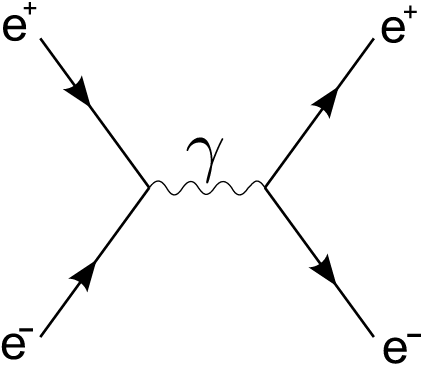
\includegraphics[width=0.35\textwidth]{fig/chapt2/electromagnetic.png}
%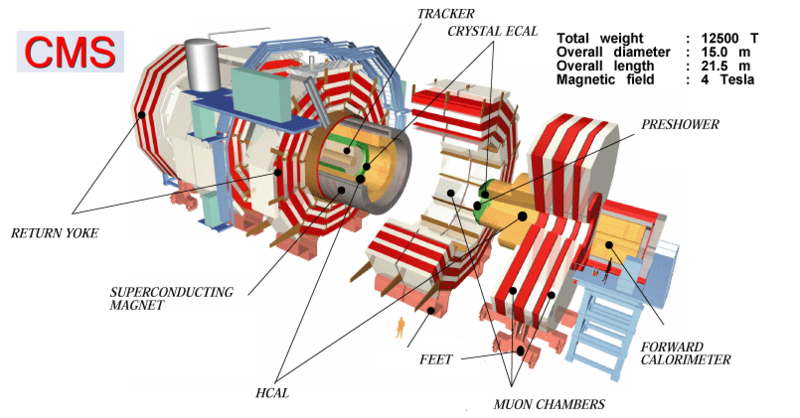
\includegraphics[scale=0.4, trim=20 50 60 30,clip]{fig/chapt3/CMS_exper.png}
\caption{\label{fig:electro_force} An overview of the Bhabha scattering in QED.}
\end{figure}
\item{\textbf{Weak Interaction}}:
All fundamental particles except gluon (g) and photon ($\gamma$) experience undergoes weak interaction by exchanging or producing W$^{\pm}$ or Z bosons. It is a short range (10$^{-17}$ to 10$^{-16}$m) interaction and responsible for many phenomena like radioactivity and quark spin flipping. Weak isospin (Y$_{3}$) conserves in weak interaction and plays a similar role in weak interaction as colour in strong interaction and charge in electromagnetism. In case of leptons, the theory is very clear, like the decay of muon mediated by W$^{-}$ boson ($\mu^{-} \rightarrow e^{-} + \nu_{\mu} + \bar{\nu_{e}}$) and electron-neutrino scattering via Z boson ($\nu_{\mu} + e^{-} \rightarrow \nu_{\mu} + e^{-}$). The lepton number conserve in both processes. A similar model applied to the three generation of quarks where a quark converts into same generation but in nature across generation conversion observed. The dilemma was solved by introducing the 3 $\times$ 3 $\textbf{CKM}$ (Cabibbo–Kobayashi–Maskawa) matrix \ref{eq:ckm1}, very near to unitary.
\begin{equation}\label{eq:ckm1}
\left({\begin{array}{ccc} \rm d' \\ \rm s' \\ \rm b' \end{array}}\right) = 
	  \left( \begin{array}{ccc}
      \rm  V_{ud} &\rm V_{us} &\rm V_{ub}\\
      \rm  V_{cd} &\rm V_{cs} &\rm V_{cb}\\
      \rm  V_{td} &\rm V_{ts} &\rm V_{tb}\end{array} \right)
\left({\begin{array}{ccc} \rm d \\ \rm s \\ \rm b \end{array}}\right)
\end{equation}  
The down type quarks ($\rm d', \rm s', \rm b'$) is a superposition of down type quarks following Equ.\ref{eq:ckm1} and couple to up type quarks via charged current weak interaction. The matrix elements gives the rate at which one quark convert to another e.g $\rm V_{ud}$ gives the transition rate of $d \rightarrow u$. All the nine CKM matrix values are given in \ref{eq:ckm2}.
\begin{equation}\label{eq:ckm2}    \small 
\rm V_{\rm CKM}	=  \left( \begin{array}{ccc}
      \rm  0.97434_{-0.00012}^{+0.00011} &\rm 0.22506\pm 0.0005&\rm 0.00357\pm 0.00015\\
      \rm  0.22492\pm 0.0005 &\rm 0.97351\pm 0.00013 &\rm 0.0411\pm 0.0013\\
      \rm  0.00875_{-0.00033}^{+0.00032} &\rm 0.0403\pm 0.0013 &\rm 0.99915\pm 0.00005\end{array} \right)
\end{equation}
The diagonal elements are $\approx$1, show the transition in the same generation is dominant \cite{ckm}.\item{\textbf{The Electroweak Symmetry:}}
The electromagnetic and weak forces were combined by Glashow, Weinberg and Salam in a unique gauge electroweak theory (GWS) based upon the $SU(2)_{L}\times U(1)_{Y}$ group \cite{gws}. The theory introduces three SU(2)$_{L}$ gauge bosons W$^{i}_{\mu}$, i = 1,2,3, with coupling strength g$_{w}$ and one U(1)$_{Y}$ gauge boson, B$_{\mu}$ with coupling constant g$'$/2. The GWS theory depends upon the chirality of particles that means it transforms left-handed particles as doublets with weak isospin (I) $\pm\frac{1}{2}$ and right-handed particles as singlet with I = 0. The hypercharge (Y) and the third component of weak isospin (I$^{3}$) are related to charge (Q in unit of e) as:
\begin{equation}\label{eq:}
Q = I^{3} + \frac{1}{2}Y
\end{equation}  
The wave function of the charged fields W$^{\pm}_{\mu}$, neutral field Z$_{\mu}$ and photon A$_{\mu}$ is represented by:
\begin{equation}\label{eq:electroweak}
\begin{split}
W^{\pm}_{\mu} = \frac{1}{\sqrt{2}}\left( W_{\mu}^{1} \mp W_{\mu}^{2}\right)\\
Z_{\mu} = \left( W_{\mu}^{3}\cos\theta_{w} - B_{\mu}\sin\theta_{w}\right)\\
A_{\mu} = \left( W_{\mu}^{3}\sin\theta_{w} + B_{\mu}\cos\theta_{w}\right)
\end{split}
\end{equation}   
where $\theta_{w}$ is the weak mixing angle given in term of electromagnetic coupling constant (g$_{e}$) as:
\begin{equation}
g_{w}\sin\theta_{w} = g'\cos\theta_{w} = g_{e} 
\end{equation} 
In GWS theory, breaking of the underlying $SU(2)_{L}\times U(1)_{Y}$ symmetry predicts the existence of two charged guage fields and two neutral guage fields shown in Equ.\ref{eq:electroweak}.  
\item{\label{item:higgs_mechanism}\textbf{The Higgs Mechanism:}} SM is based on gauge invariance which forbids to introduce explicit mass terms in the Lagrangian of a chiral theory, as it breaks the symmetry. This results to massless SM particles, a contradiction to the nature. A mechanism is needed to introduce mass term in the SM without spoiling guage symmetry known as Higgs Mechanism also called Brout-Englert-Higgs (BEH) mechanism \cite{eng_brout,p_w_higgs}. The GWS uses the BEH mechanism which introduces a new doublet of complex scalar field, known as Higgs field, preserves symmetry under the gauge transformations, and acquires a non-zero vacuum expectation value, spontaneous electroweak symmetry breaking. The Higgs field contains a total of four additional degrees of freedom where three of them become massive, given in \ref{eq:electroweak}, after breaking the symmetry and one remains massless, the photon $\gamma$. The Higgs doublet introduces in the SU(2)$_{L}$ with hypercharge (Y = $\frac{1}{2}$) is in the form of,
\begin{equation}
\phi = \Big(\begin{array}{c}
\phi^{+}\\
\phi^{0} \end{array}\Big)
= \frac{1}{\sqrt{2}}
\Big(\begin{array}{c}
\phi^{1} + i\phi^{2}\\
\phi^{3} + i\phi^{4}
\end{array}\Big)
\end{equation}
The SM electroweak Lagrangian density is given in term of
\begin{equation}\label{eq:beh_lagrange}
\mathcal{L}_{BEH} = (D^{\mu}\phi)^{\dagger}(D_{\mu}\phi) - V(\phi), \quad \textrm{with}\quad 
        V(\phi) = \mu^{2}\phi^{\dagger}\phi + \lambda(\phi^{\dagger}\phi)^{2}
\end{equation}
where first term of the lagrangian D$^{\mu}$ corresponds to the covariant derivative of the Higgs field under the SU(2) $\times$ U(1) group and the second term is the scalar potential known as "Mexican Hat" potential, shown graphically in Fig.\ref{fig:mexican_hat}. 
\begin{figure}[h]
\centering
\captionsetup{width=0.8\linewidth}
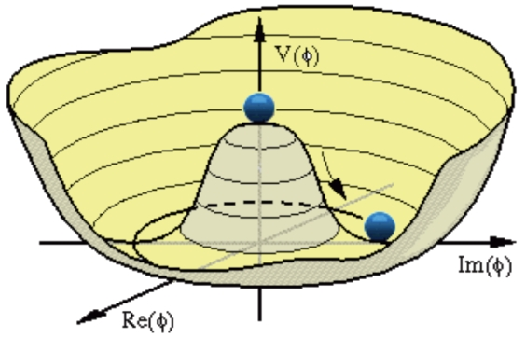
\includegraphics[width=0.4\textwidth]{fig/chapt2/mexican_hat.png}
%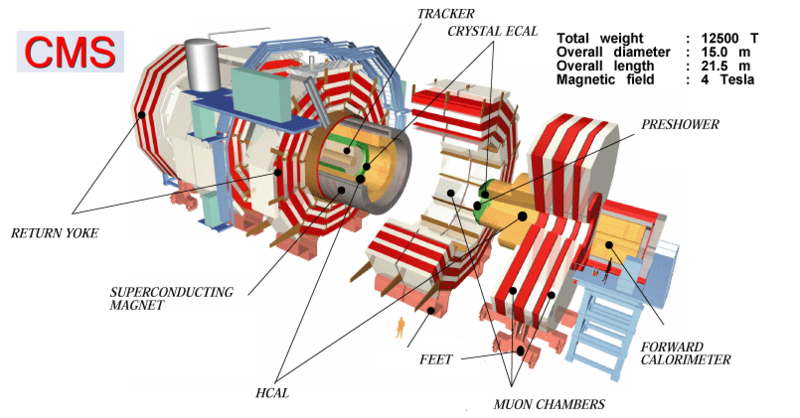
\includegraphics[scale=0.4, trim=20 50 60 30,clip]{fig/chapt3/CMS_exper.png}
\caption{\label{fig:mexican_hat}The scalar potential V($\phi$)with $\mu^{2}$ < 0 has a "Mexican hat shape, with the minimum in a rim around the origin. Moving from the origin down to the minimun, the symmetry breaks and the scalar field acquire a vacuum expectation value (vev) in the process}
\end{figure}
The higgs potential has chosen in the simplest form to achieve the necessary spontaneous symmetry breaking, while being renormalizable. The Higgs potential V($\phi$) depends on the values of $\lambda$ and $\mu^{2}$. For a stable vacuum, the parameter $\lambda$ has to be a positive value. If $\mu^{2}$ > 0, the scalar potential has a global minimum, $\langle 0\abs{\phi}0\rangle = 0$, where no spontaneous symmetry breaking occurs; while for $\mu^{2} < 0$ the symmetry breaks and the Higgs field acquires a non zero vacuum expectation value with conditions $\langle 0\abs{\phi}0\rangle = \frac{-\mu^{2}}{2\lambda} = \frac{\nu}{\sqrt{2}}$ where $\nu = \sqrt{-\frac{\mu^{2}}{\lambda}}$ is the vev. The scale of electroweak symmetry breaking is related to the W boson mass and to the Fermi constant G$_{F}$:
\begin{equation}
\nu = 2\frac{m_{w}}{g_{w}} = (\sqrt{2}G_{F})^{-\frac{1}{2}} \approx 240 GeV 
\end{equation}
The Higgs field can be re-defined in terms of a perturbation around its non-zero vev by inserting a new scalar field h(x):
\begin{equation}\label{eq:higgs_state}
\phi(x) = \frac{1}{2}\left(\begin{array}{c}
0\\
\nu + h(x)
\end{array}\right)
\end{equation}
The new scalar field corresponds to the Higgs particle with mass $m_{h} = \nu\sqrt{2\lambda}$ and no charge. Rearranging Equ.\ref{eq:beh_lagrange} by inserting $\phi$ from \ref{eq:higgs_state} and defining the bosonic states shown in \ref{eq:electroweak} we can see that the three bosons (W$^{\pm}$, Z$^{0}$) acquire masses while photon $\gamma$ remains massless.
\begin{equation}
m_{W}^{2} = \frac{\nu^{2}g^{2}}{4} ; m_{Z}^{2} = \frac{\nu^{2}(g^{2} + g'^{2})}{4} ; m_{\gamma} = 0 
\end{equation}
The concept of the gauge boson mass terms can be further extended to the mass terms of the fermions in a different way that would also break the local gauge invariance of the theory. This can be done by introducing the Yukawa coupling $\lambda_{f}$ between the fermions fields and the Higgs boson with the coupling constant proportional to the respective fermion mass. We get,
\begin{equation}
m_{f} = \frac{\lambda_{f}}{\sqrt{2}}\nu
\end{equation}
In SM, neutrinos are considered massless.
The Higgs mechanism successfully serves in the GWS model to give masses to weak bosons and predict a new scalar particle, the Higgs boson. In 2012, both CMS and ATLAS discovered the Higgs boson that confirmed the symmetry breaking in nature.
\end{itemize}

\subsection{The Top Quark}
Top quark belongs to the third generation of quarks, the heaviest known elementary particle in the SM, and with its unique properties has long been considered of potentially carrying key information that may lead to answer some of the basic open questions in particle physics. The CDF and D0 collaborations at the Tevatron in 1995 bring the long quest of the sixth and last quark of the SM to an end by the discovery of top quark \cite{top_quark}. The mass of the top quark measured to be 173.5 and has very short life time $\approx$ 10$^{-23}$s, less than the time of hadronization that enables the top quark to decay before forming bound state. The LHC started data taking in 2010 at $\sqrt{s}$ = 7 TeV and after the three years of data taking by CMS and ATLAS, about a million of top quark events we recorded which named the LHC as “top factory”. All the current results of the top quark production, decay and coupling are consistent with the Standard Model prediction and no clue of physics beyond Standard Model have been observed in its properties. However different studies are underway to search for new physics especially in the $t\bar{t}$ resonance and interference production. The interference pattern comes into play when the SM $t\bar{t}$ background interfere with the signal (decay of the scalar or pseudo-scalar into $t\bar{t}$). The focus of this thesis is the search for heavy scalar and pseudo-scalar decaying into $t\bar{t}$ where $t\bar{t}$ further decays leptonically. Both resonance and interference are studied in detail. 
\begin{figure}[h]
\centering
%\captionsetup{width=0.8\linewidth}
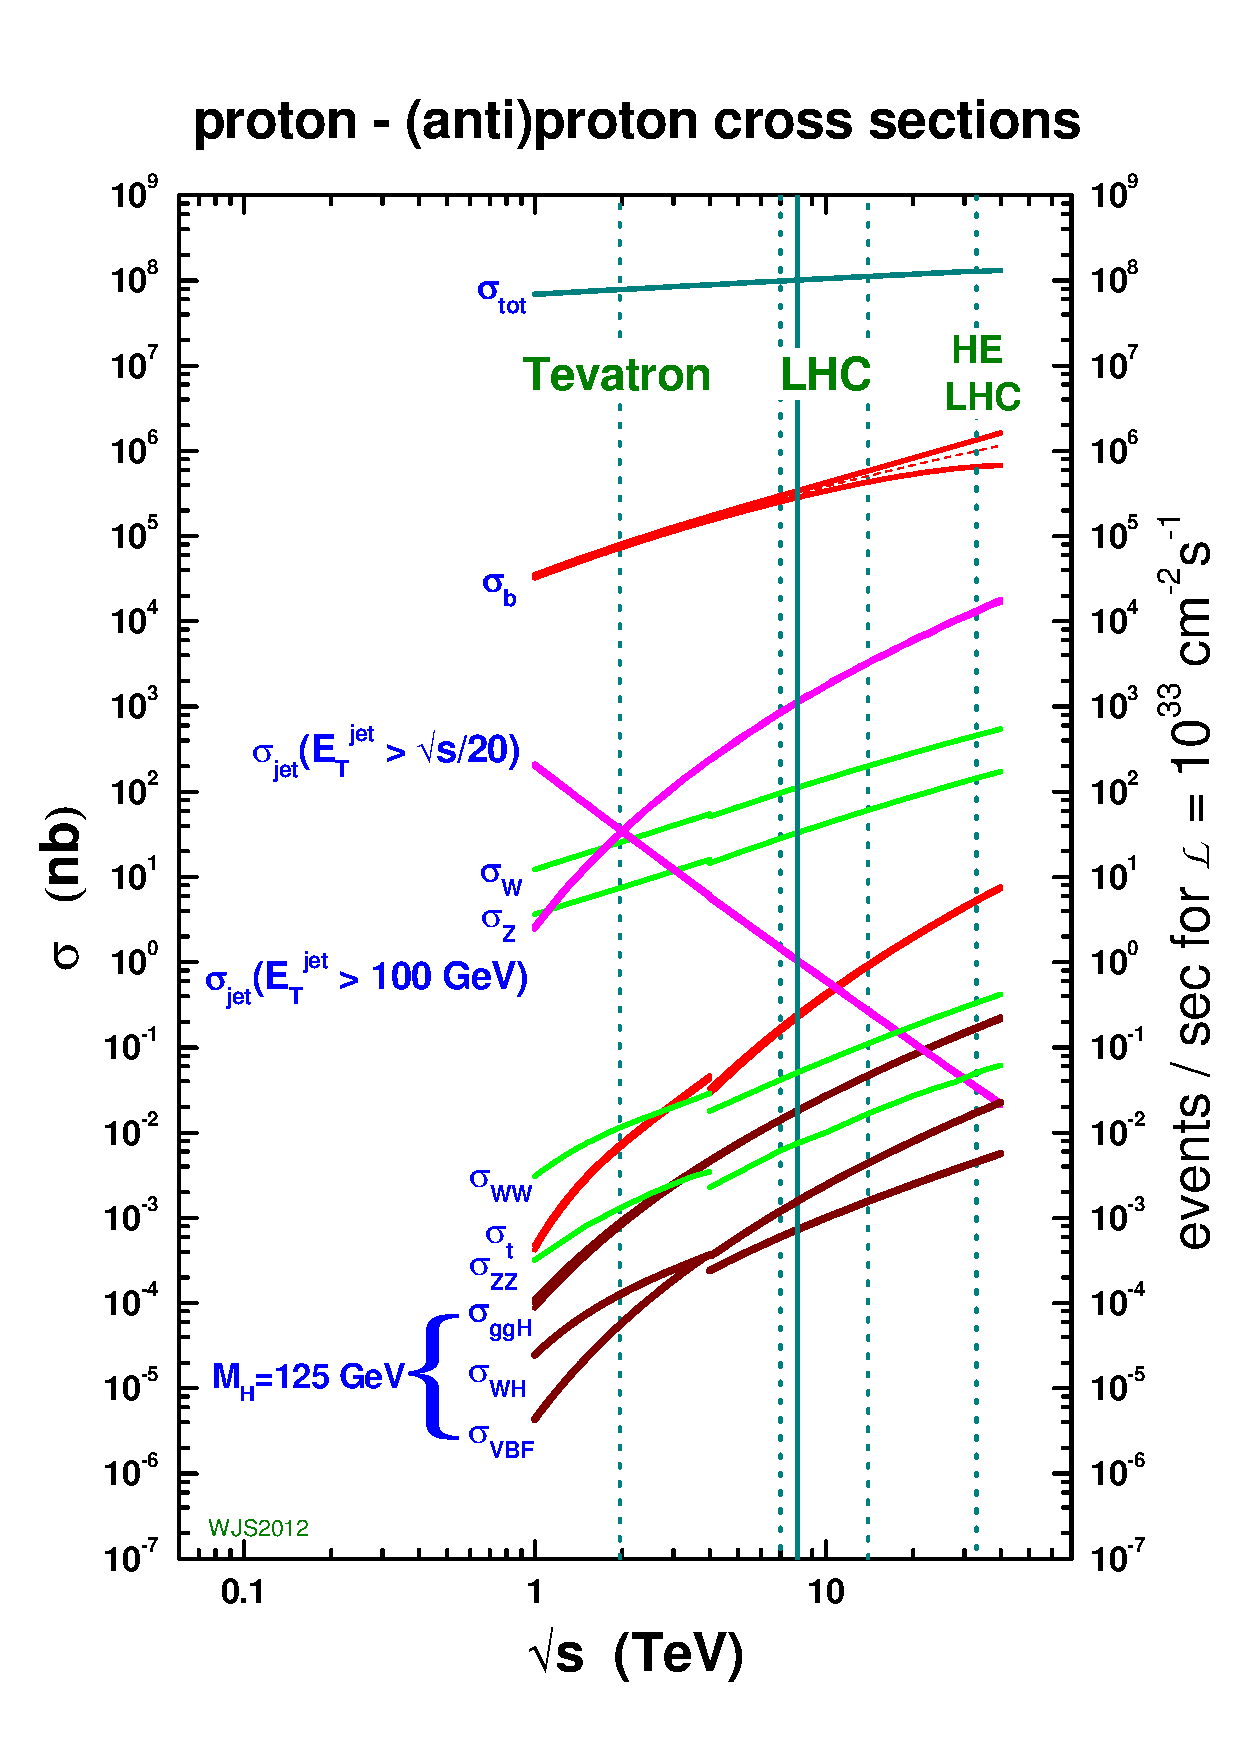
\includegraphics[width=0.6\textwidth]{fig/chapt2/crosssections2012HE_v4.pdf}
%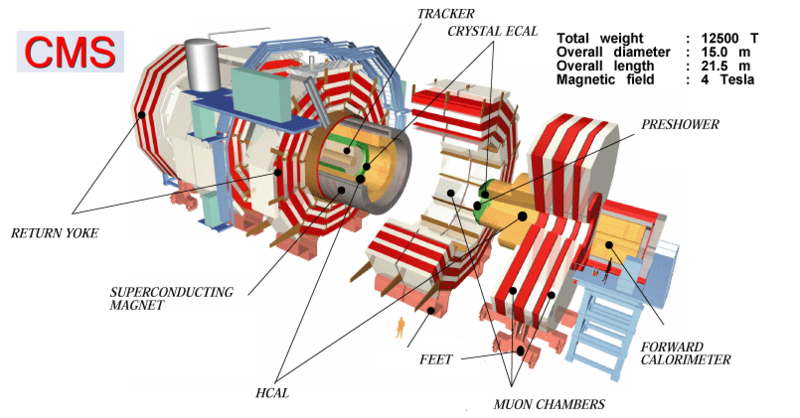
\includegraphics[scale=0.4, trim=20 50 60 30,clip]{fig/chapt3/CMS_exper.png}
\caption{\label{fig:lhclumi_plot}The Standard Model cross sections as a function of energy \cite{lhclumi_plot}.}
\end{figure}
\subsubsection*{Top quark production}
At hadron colliders, two mechanisms are responsible for the top quark production, $t\bar{t}$ pairs via strong interaction and single top production via electroweak process, where $t\bar{t}$  is the most abundant production at high energy regime. The production of $t\bar{t}$ is contributed by the two LO processes at tree level shown in Fig.\ref{fig:ttbar_prod}: quark–antiquark ($q\bar{q}$) annihilation and gluon–gluon (gg) fusion in the s-, t-, and u-channel. In $p\bar{p}$ collider such as Tevatron, the dominant production mode for $t\bar{t}$ is the $q\bar{q}$ annihilation while for $pp$ collider like LHC, $gg$ fusion more likely takes place. The hadronic production cross section of the $t\bar{t}$ pair is successfully explained by the QCD and obtained from the proton-proton interaction using the factorization theorem \cite{ttbar_production} read as:
\begin{equation}
d\sigma_{pp\rightarrow t\bar{t}}(s,m_{t}) = \sum\limits_{i,j=q,\bar{q},g}\int dx_{i}dx_{j}f_{i}(x_{i},\mu^{2}_{f})f_{j}(x_{j},\mu^{2}_{f}).\hat{\sigma}_{ij\rightarrow t\bar{t}}(\hat{s}, m_{t}, \mu_{f},\mu_{r}, \alpha_{s}))
\end{equation}
The cross sections are integrated over all partons participating in the scattering process with momentum fractions x$_i$ and x$_j$ with respect to the proton momenta and summed over all parton type i and j. The PDFs $f_{i}(x_{i}, \mu^{2}_{f})$ are partonic distribution functions, describe the probability to find a parton i inside a hadron in momentum range x to x+dx. The PDFs absorbs all types of long-distance effects of partons inside the hadrons whereas the hard scattering partonic cross section $\hat{\sigma}$ represents the actual hard process at small distances which can be computed in perturbative QCD. The long and short distance processes can be separated by introducing a new energy scale called “factorization scale ($\mu_{f}$)” on which both PDFs and $\hat{\sigma}$ depend. The hard scattering partonic cross section $\hat{\sigma}$ further depends on the partonic center-of-mass energy $\hat{s} = x_{i}x_{j}s$ (s is the pp CoM energy squared), the renormalization scale $\mu_{r}$, to treat ultraviolet divergence, and the strong coupling constant $\alpha_{s}$. Both energy scales, $\mu_{f}$ and $\mu_{r}$, are set to the physical energy scale of the process, like for $t\bar{t}$ pair production cross section, they are set to the top quark mass; $\mu_{f} = \mu_{r} = m_{t}$. The recent measurement of $\sigma(t\bar{t})$ at CMS resulted 889 $\pm$ 2 (stat)$^{+26}_{-28}$ (syst) $\pm$ 20 (lumi) pb,  in agreement with the standard model prediction\cite{top:16_006}.\\
\begin{figure}[h]
\centering
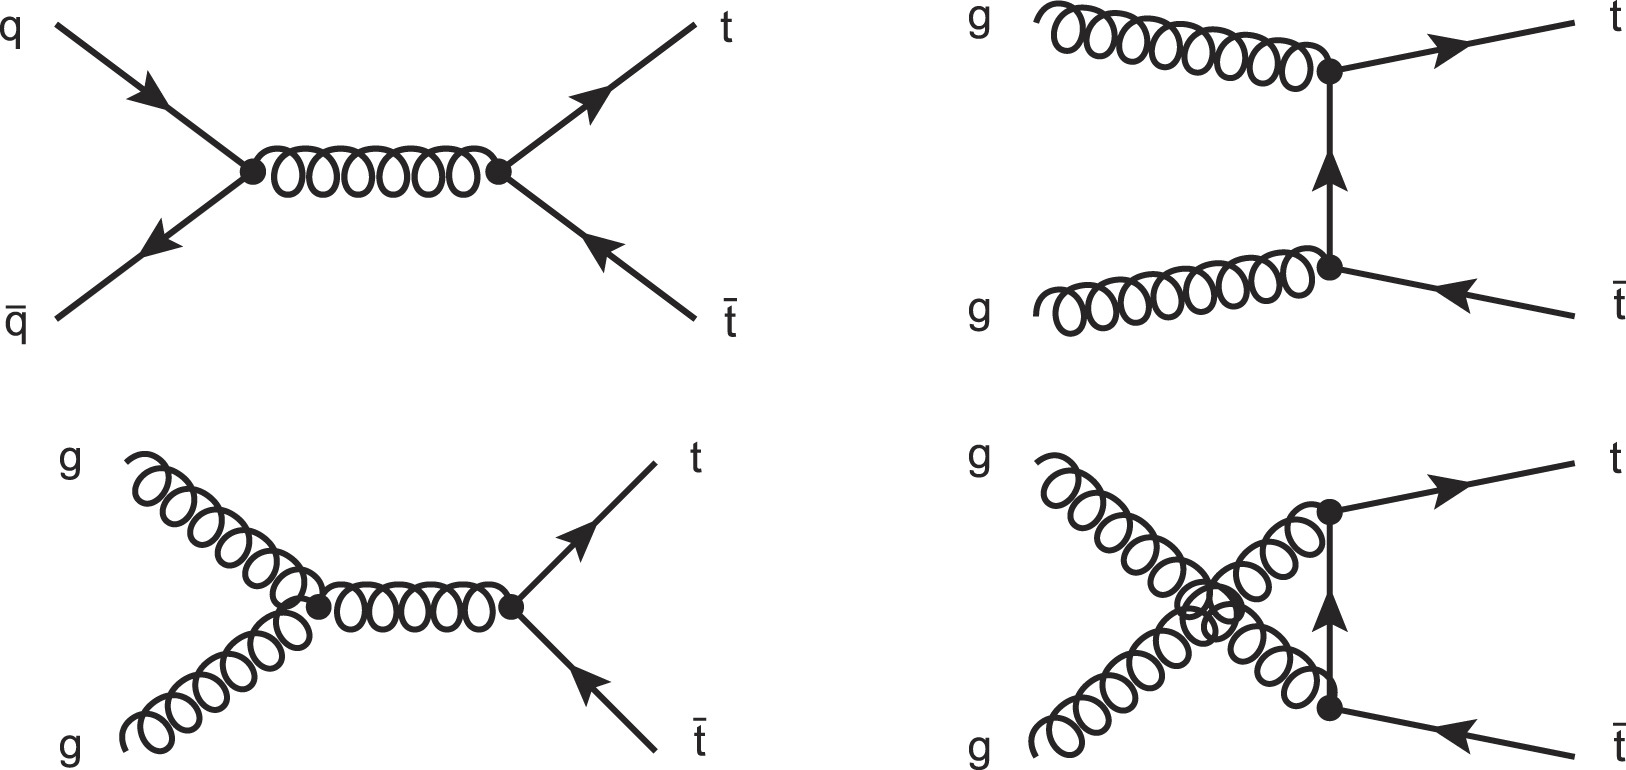
\includegraphics[width=0.7\textwidth]{fig/chapt2/ttbar_productions.jpg}
\caption{\label{fig:ttbar_prod}$t\bar{t}$ pair production in QCD at LO: top left is $q\bar{q}$ annihilation, bottom left is gg fusion in the s-channel, top right is gg fusion in the t-channel and bottom right shows gg fusion in the u-channel.}
\end{figure}
Single-top can be produced at hadron colliders via three different electroweak processes, t-channel (the dominant channel with 70\% of the total cross section), the associated production of a top ($\bar{t}$) quark and a W boson (tW-channel with 25\% cross section) and the s-channel (5\% of the total cross section). The electroweak production vertex includes the CKM matrix element V$_{tb}$ that makes the single top processes more interesting for SM and BSM physics.
\subsubsection*{Top quark decay}
The top quark almost exclusively decays into a W-boson and a b-quark via the electroweak interaction due to the CKM matrix element V$_{tb} \approx$ 1. Compare to other quarks of the SM, top quark has very short life time ($\tau_{t} \approx 5 \times 10^{-25}$s) and decays before hadronization ($\tau_{had} \approx 10^{-24}s$). This makes the top quark more interesting to be studied in bare state and its kinematic and dynamic information, like spin correlation, transfers to its decay products without diluted by hadronization. The decay of $t\bar{t}$ system can be classified on the basis of W boson decay products where W boson can decay into a pair of light quarks, with BR($W \rightarrow q\bar{q}') \simeq 67\%$, or charged leptons with corresponding neutrino of the same generations with BR($W \rightarrow l\nu_{l}) \simeq 33\%$. At first order, the possible decay modes of a $t\bar{t}$ event can be grouped into three main categories given in table\ref{table:ttbar_decay}
\begin{table}[h]%\footnotesize
\centering
     %\begin{tabular}{|p{1.4cm}|p{1.0cm}|p{1.0cm}|}
    \tabulinesep=1.0mm
     \begin{tabu}{|l|c|c|}
        \hline
        Channel & Decay mode & BR\\
\hline 
Hadronic & $t\bar{t}\rightarrow b\bar{b}W^{+}W^{-}\rightarrow b\bar{b}q\bar{q}'q''\bar{q}'''$ & 46\%\\ 
\hline
Semileptonic & $t\bar{t}\rightarrow b\bar{b}W^{+}W^{-}\rightarrow b\bar{b}q\bar{q}'l\nu_{l}$ & 45\%\\ 
\hline
Dileptonic & $t\bar{t}\rightarrow b\bar{b}W^{+}W^{-}\rightarrow b\bar{b}ll'\nu_{l}\nu_{l'}$ & 9\%\\
\hline
\end{tabu}
     \caption{Three categories of $t\bar{t}$ sytem decay with branching ratios\cite{ttbar_decay_ratio}.\label{table:ttbar_decay}}
%\end{center}
\end{table}  

\begin{figure}[htp]
\centering
\begin{tabular}{cc}
\hspace{-0.3cm}
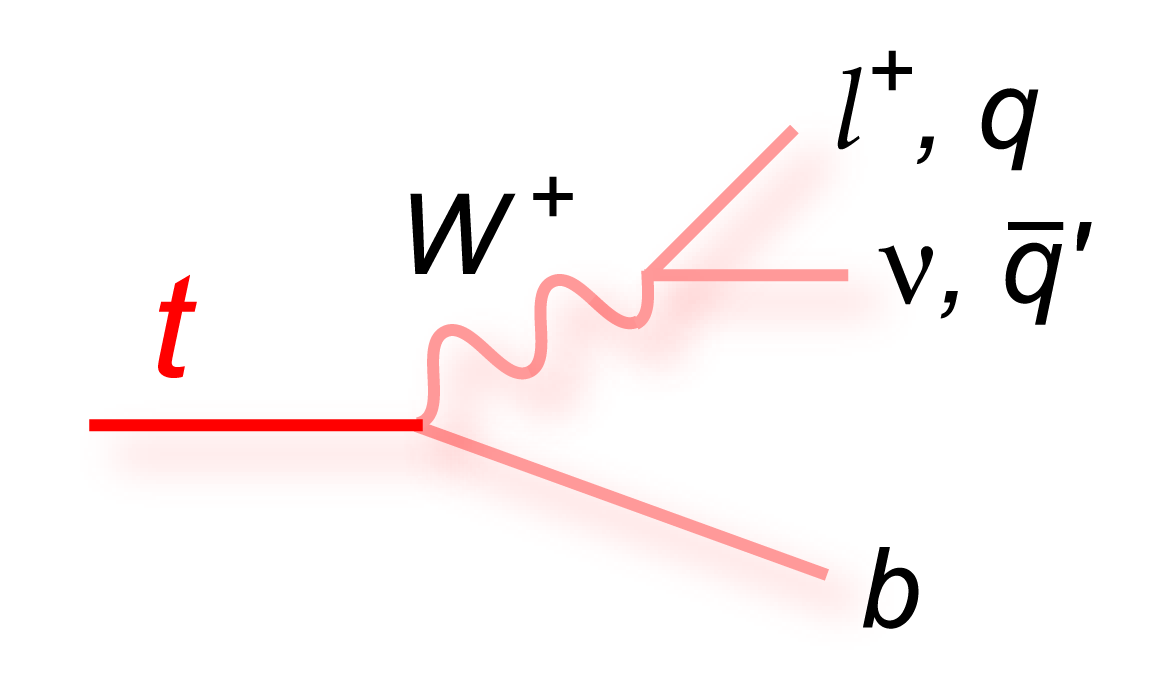
\includegraphics[scale=0.19]{fig/chapt2/single_top_decay.png}
& \hspace{-0.5cm} 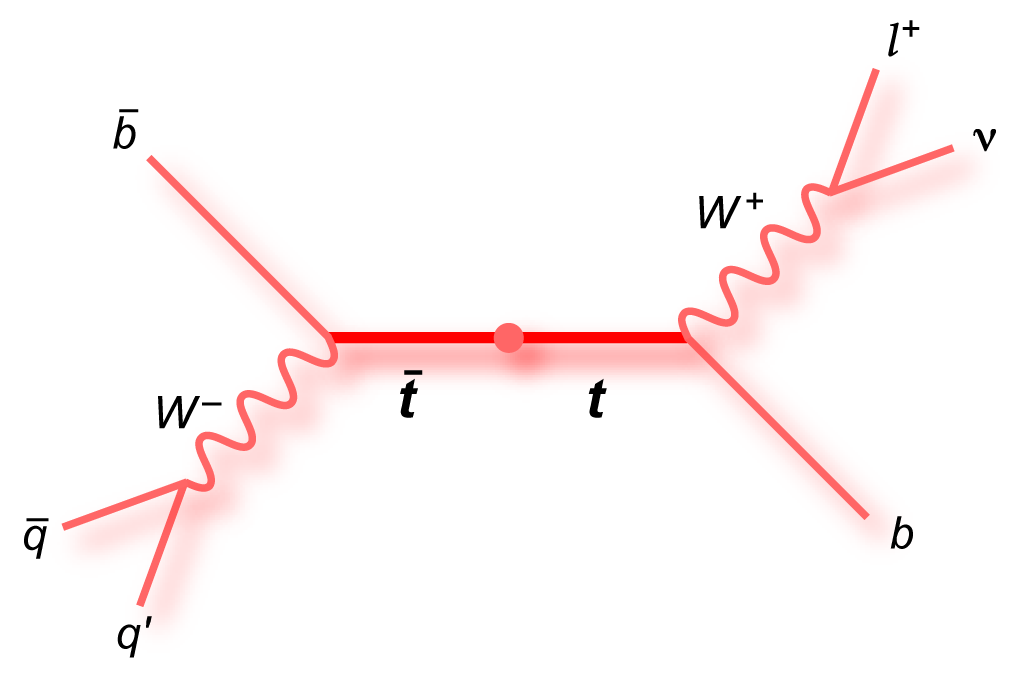
\includegraphics[scale=0.19]{fig/chapt2/ttbar_decay.png}\\
   ($\mathbf{a}$)\qquad\qquad\qquad&($\mathbf{b}$)\qquad\\
\end{tabular}
\caption{Feynman diagram for sigle top quark decay (a) and the semileptonic decay of $t\bar{t} $ (b).}\label{fig:top_decay}
\end{figure}
\begin{itemize}
\item {\textbf{Hadronic Channel:}}
Both W bosons coming from $t\bar{t}$ event decay into light quark-antiquark pairs (quark and antiquark further hadronized in the form of jets) with high branching fraction, resulted to a large sample of selected events. In this channel at least six jets are needed, two of them are stemming from bjets and remaining from light jets. In hadron colliders like LHC, this channel  suffers from an overwhelming QCD multijet background, whose cross section is orders of magnitude higher than the one for $t\bar{t}$ production. The QCD multijet background is difficult to model from simulation which requires data driven technique to take it from data.
\item{\textbf{Dileptonic Channel:}}
In dileptonic channel, both of W bosons decay leptonically, resulting two bjets, two charged leptons and two corresponding neutrinos in $t\bar{t}$ event. It has the lowest branching ratio but a very clean signature at the experimental level due to the presence of two oppositely charged leptons, which can be easily distinguished from QCD multijet events. The disadvantage of dileptonic event is the presence of two neutrinos, considered as the missing transverse energy in the event, where $t\bar{t}$ can’t be reconstructed perfectly. 
\item{\textbf{Semileptonic Channel:}}
Finally, the lepton+jets channel whose decay chain is shown in Fig.\ref{fig:top_decay}b, is a good compromise between a reasonable
BR and relatively clean experimental signature with reconstructable tt-event topology (especially when lepton = $\mu$, e). The semileptonic channel is restricted to $\mu$ + jets and e + jets as the $\tau$ lepton further decay into charged lepton and neutrino or jets which makes the channel more complicated. Therefore a dedicated study is needed to take into account the $\tau$ + jets channel.
 
With clean signature and adequate BR ($\sim$30\%), the lepton+jets channel has chosen for this thesis. In the resolved case, where final products of each top quark ($P_{T} \le 400GeV$) are reconstructed as separate objects, the $t\bar{t}$ final objects consists of four jets, one charged lepton (muon or electron) and neutrino. Two of the jets are tagged as bjets, arise directly from the decay of top quark while two of light jets coming from one of the W-boson. The second W-boson decays into a charged lepton and corresponding neutrino. As neutrino escapes without detection, it is treaded as missing transverse energy ($E^{miss}_{T}$) in the event. The longitudinal component of $E^{miss}_{T}$ is unmeasured which can be reconstructed using analytical solution explained in detail in Sec.\ref{https://arxiv.org/pdf/1305.1878.pdf}. The $t\bar{t}$ system is reconstructed using Rochester Algorithm explained in Sec.\ref{https://cds.cern.ch/record/2141097/files/TOP-16-008-pas.pdf}.      
\end{itemize}
\subsection{The SM Higgs Boson}
In early 60's, the existence of the Higgs boson was theoretically predicted by Robert Brout, Fran\c cois Englert and Peter Higgs using the well known BEH mechanism \ref{item:higgs_mechanism}. The main goal in the field of particle physics during the last few decades was the Higgs boson discovery, where a number of searches have been conducted at the Large Electron-Positron Collider (LEP) at CERN and at Fermilab with the experiments CDF and D0 at $\sqrt{s} = 1.96$ TeV using an integrated luminosity of 10.0 fb$^{-1}$. The later narrowed down the mass range by excluding two regions: 100 < m$_{H}$ < 130 GeV/c$^{2}$ and 147 < m$_{H}$ < 180 GeV/c$^{2}$, at the 95\% C.L. Furthermore, they observed a significant access of data events with respect to the background estimation in the
mass range, 115 < m$_{H}$ < 140 GeV/c$^{2}$ \cite{sm_higgs_fermilab}. The official announcement of the higgs boson discovery with 5$\sigma$ significance made by the CERN experiments, CMS and ATLAS, in July 2012 by combining data of 7 and 8 TeV energy with integrated luminosity of 10.4 fb$^{-1}$ by CMS and 10.6 fb$^{-1}$ by ATLAS \cite{cms_sm_higgs,atlas_sm_higgs}. The search performed in five higgs decay modes: $\gamma\gamma$, ZZ, W$^{+}$W$^{-}$, $\tau^{+}\tau^{-}$ and $b\bar{b}$ where excess is most significant in the two decay modes with the best mass resolution, $\gamma\gamma$ and ZZ. By performing a fit to the signals, the mass of the higgs boson is 125.3$\pm$0.4(stat.)$\pm$0.5(syst.) GeV. At 13 TeV, the study has been repeated and the mass of the higgs boson measured to be 124.50$^{+0.48}_{-0.46}$ GeV with a constrained on width $\Gamma_{H}$ < 41 MeV \cite{sm_higgs_13tev}. The measured cross section agrees well with the expectation from the standard model. The signal strength $\mu$, defined as the production cross section of the Higgs boson times its branching fraction to four leptons relative to the standard model expectation, is measured to be; $\mu$ = 0.99$^{+0.33}_{-0.26}$ at m$_{H}$ = 125.09 GeV. The higgs boson properties like spin, parity, the ratios of production rates for different production modes, the ratios of couplings to fermions and vector bosons etcetera are well agree with the standard model prediction. The higgs mass measured at 13 TeV using 12.9 fb$^{-1}$ data in two channels $H\rightarrow\gamma\gamma$ (a) and $H\rightarrow ZZ\rightarrow 4l$ (b) is shown in figure \ref{fig:sm_higgs} where excess in data is clear around 125 GeV is visible. 
   
\begin{figure}[htp]
\centering
\begin{tabular}{cc}
\hspace{-0.3cm}
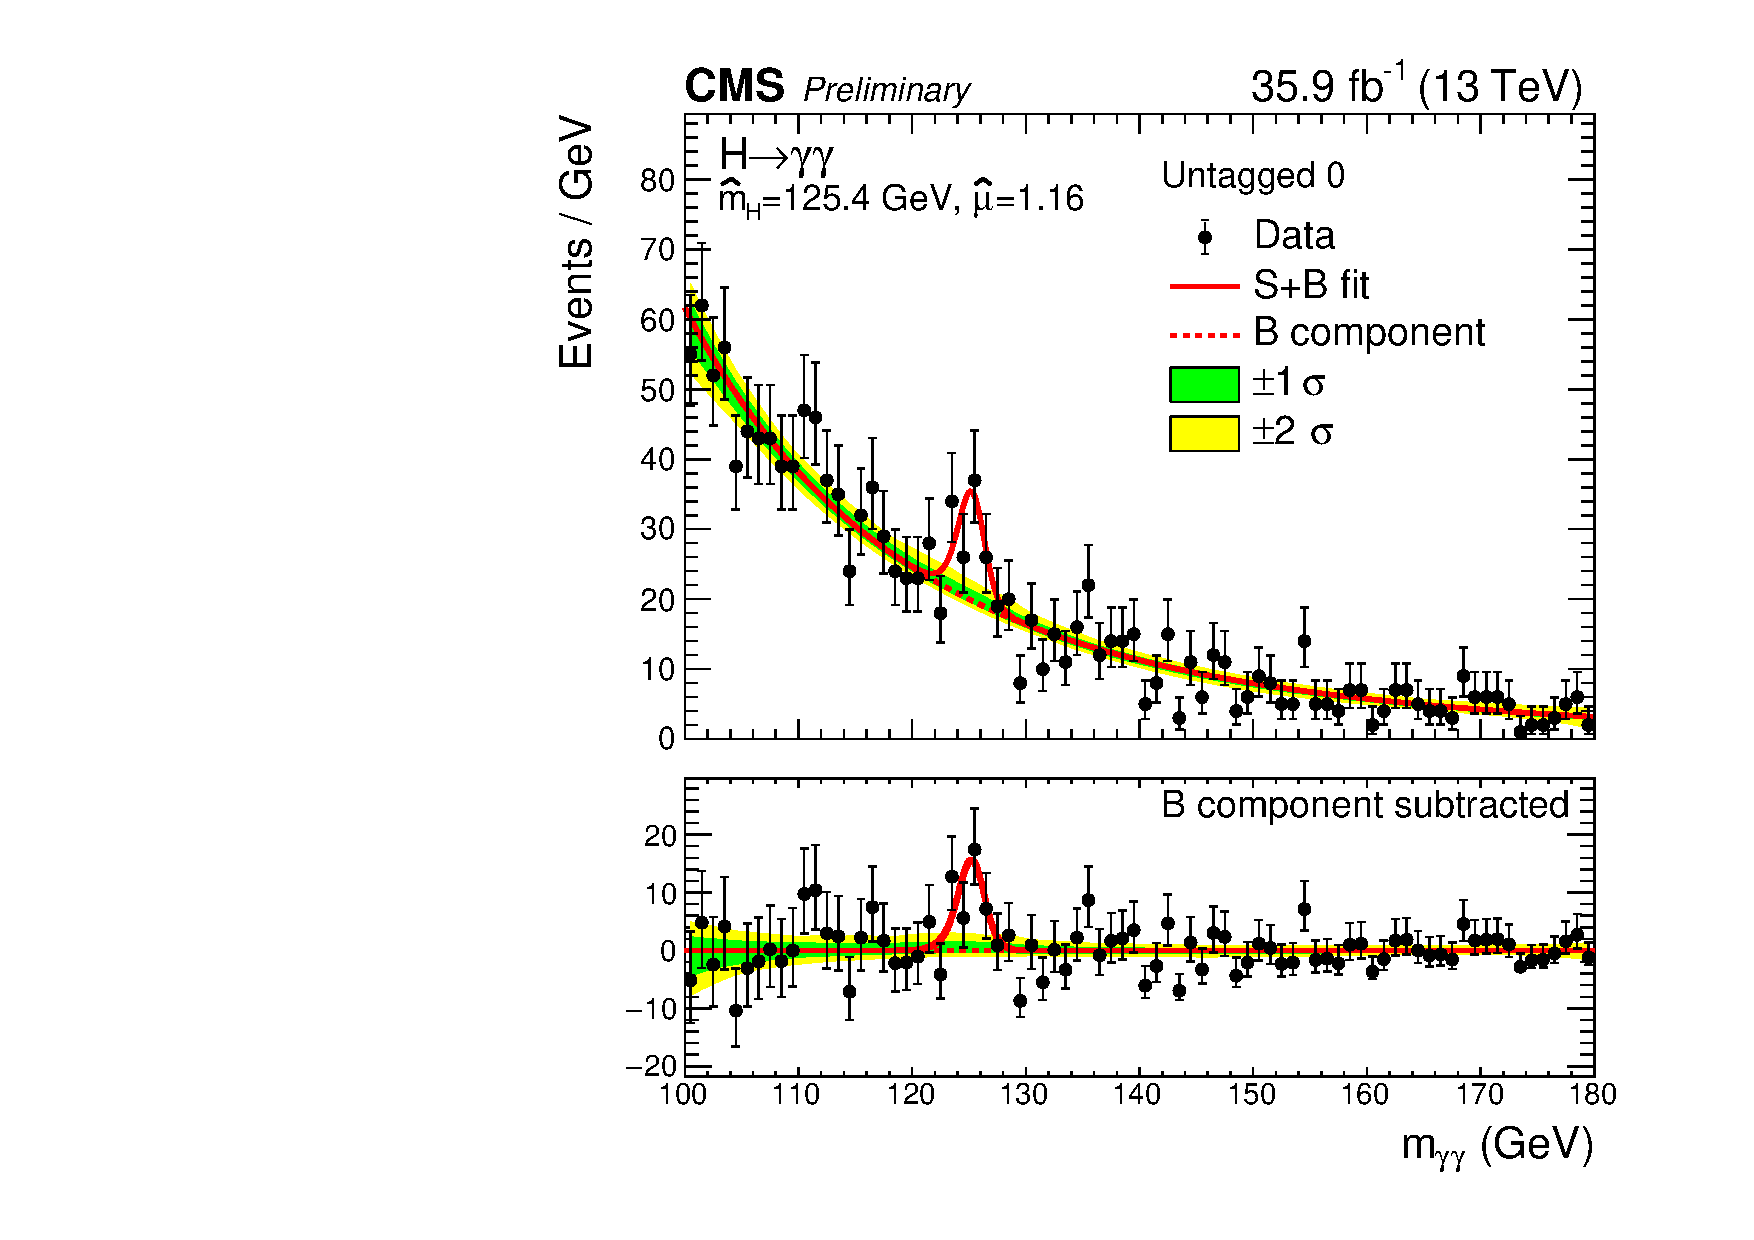
\includegraphics[scale=0.35]{fig/chapt2/CMS-PAS-Htogamma.pdf}
& \hspace{-0.5cm} 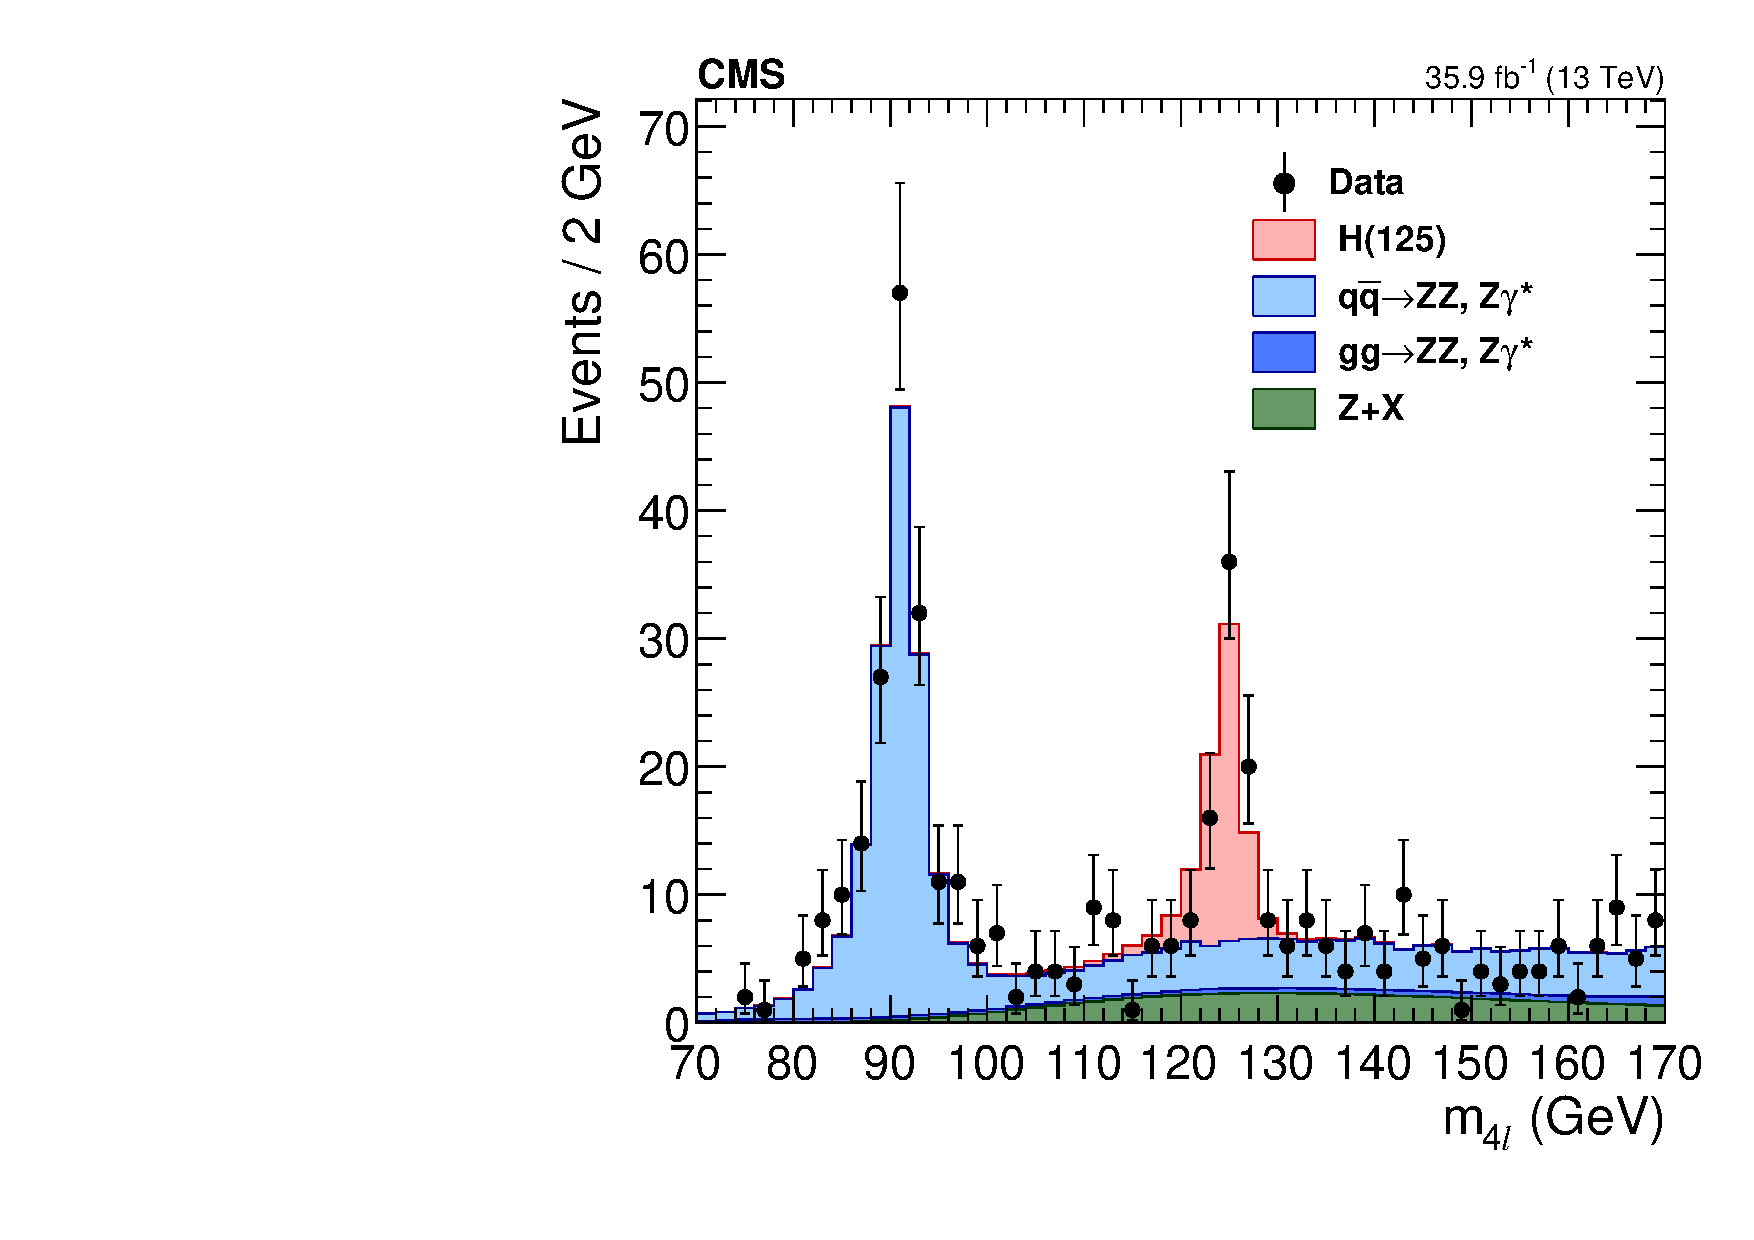
\includegraphics[scale=0.35]{fig/chapt2/CMS-PAS-Hto4l.pdf}\\
   ($\mathbf{a}$)\qquad&($\mathbf{b}$)\qquad\\
\end{tabular}
\caption{\label{fig:sm_higgs}The SM Higgs mass spectra obtained in the 2016 CMS search using the two most sensitive decay channels, di-photon (left) and four-lepton (right). Both channels show larger than 5 standard deviations significance of the observed signals around 125 GeV and the data correspond to an integrated luminosity of 13 fb$^{-1}$, collected with the CMS detector at a centre-of-mass energy of 13 TeV \cite{pub:sm_higgs4l,pub:sm_higgs2gamma}.}
\end{figure} 

\begin{itemize}
\item{\textbf{Production and decay of the SM Higgs boson:}} The SM higgs boson couples to every massive particle hence production in hadron collider is possible in many ways, following four of them are the most common.
\begin{enumerate}
\item{\textbf{Gluon-gluon fusion (ggF):}} In this mode of production, two gluons interact to produce a Higgs boson mediated by heavy quarks (mainly top quark) loop as higgs boson doesn't directly couple to massless gluon. This channel of production has higher cross section through out the higgs boson mass range.
\item{\textbf{Vector boson fusion (VBF):}} In VBF mode, two quarks from colliding protons radiate massive vector bosons (W or Z) and its fusion results into the Higgs boson production. It is the second highest cross section process with 10 times less than the ggH but has a clear signature because of the pure electroweak process. 
\item{\textbf{Associated production with W$^{\pm}$ or Z$^{0}$ (VH):}} This process also known as Higgs-Strahlung, the third highest cross section, in which a massive vector boson produced by the interacting of a valence quark with an antiquark from the sea and the massive vector boson further radiates a Higgs boson. This mode is helpful to test the higgs coupling with the massive vector boson.
\item{\textbf{Associated production with $t\bar{t}$ ($t\bar{t}$H):}} In this mode of production, the higgs is associated with heavy quarks pair like top quark pair which can be initiated either by gluon-gluon fusion or $q\bar{q}$ annihilation. This channel has smaller cross section but more interesting because of the direct coupling with the top quark.
\end{enumerate} 
Higgs boson decays through many channels either direct coupling to the final state massive particles or indirectly via boson or fermion loop in massless final state particles (photon, gluon). The decay channel $H\rightarrow b\bar{b}$ has the largest branching ratio (BR) but diluted by the irreducible QCD background which mimics the signal. The same is true for $H\rightarrow \tau\bar{\tau}$ channel where $\tau$ decays hadronically. Despite the low BRs, the two channels $H\rightarrow ZZ^{\star}\rightarrow 4l$ and $H\rightarrow \gamma\gamma$ show a very clear signature to the higgs and ultimately the higgs discovery became possible using these two channels. Figure \ref{fig:sm_higgsxsec_BR} (a) shows the higgs cross section as a function of centre of mass energy for m$_{H}$ = 125 GeV with a band of theoretical uncertainty and (b) shows the BRs as a function of higgs mass with a band of total uncertainty(\%).     
\end{itemize} 
\begin{figure}[htp]
\centering
\begin{tabular}{cc}
\hspace{-0.3cm}
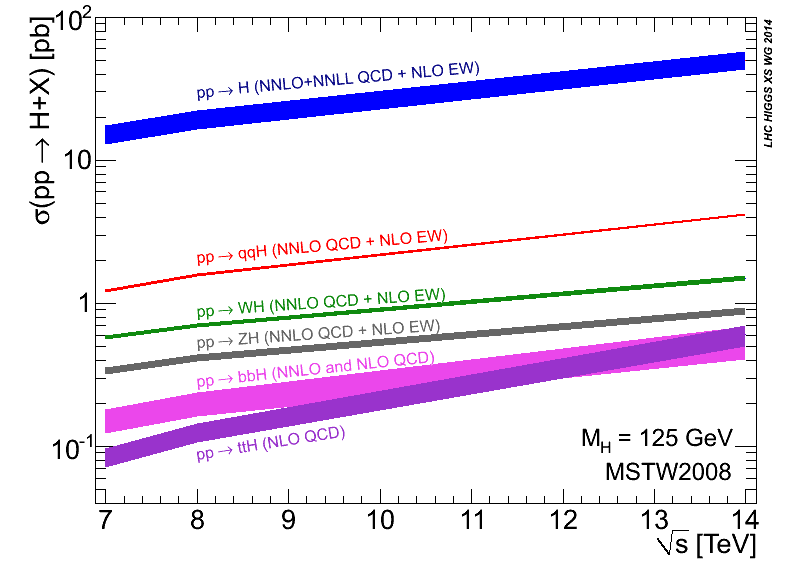
\includegraphics[scale=0.278]{fig/chapt2/7_14_xsec.png}
& \hspace{-0.5cm} 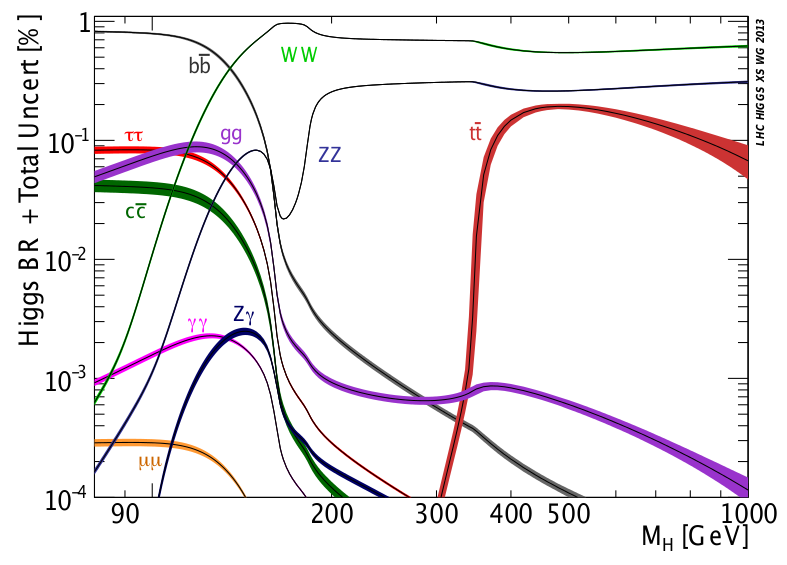
\includegraphics[scale=0.38]{fig/chapt2/Higgs_BR_RECT.png}\\
   ($\mathbf{a}$)\qquad&($\mathbf{b}$)\qquad\\
\end{tabular}
\caption{\label{fig:sm_higgsxsec_BR} Higgs boson (a): production cross section for main modes as a function of centre of mass energy exploiting m$_{H}$ = 125 GeV for $pp$ collider. (b): Branching ratio (BR) with full uncertainty in almost all channels as a function of higgs mass \cite{pub:sm_higgsxsec}.}
\end{figure} 
\section{Beyond the Standard Model}\label{sec:bsm}
Although the SM has been tested with great success in predicting and explaining many physics processes, especially in its gauge and flavour sector, but it is still not the ultimate theory as there exist a few experimental evidences and theoretical issues that are not explained by the SM. The most prominent among them are, the gravity, matter anti-matter asymmetry, the existence of dark matter and dark energy and the non-vanishing neutrino mass. There are some fundamental characteristics of the SM which we can't explain. The most important among them are: Why mass of the SM higgs boson is 125 GeV where the Plank scale is at $\mathcal{O}(10^{19})$ GeV?. This phenomenon is commonly known as hierarchy problem and a basic motivation for this search, explained in more detail in section \ref{subsec:hierarchy}. Why we have three families of fermion and they have a wide mass range?.
\subsection{The Hierarchy problem}\label{subsec:hierarchy}
Physics beyond the Standard Model can be probed by many reasons, but the core issue that is front and center for us today, relevant to Higgs boson physics and electroweak explorations at the Large Hadron Collider, is the Hierarchy Problem. The hierarchy problem involves the large difference between the Planck mass $M_{pl} \approx 10^{19}$ GeV, an energy scale associated with gravity, and the electroweak symmetry breaking scale ($10^{2}$) of the Standard Model. Higgs boson is the only fundamental scalar in the SM which can be subjected to higher order loops corrections from spin 0, 1/2 and 1 particles with a quadratic dependence on the cutoff scale (Plank scale). These corrections may take the higgs mass to the highest scale but in contrast we see the higgs mass $\sim$ 125 GeV. In case of fermions and guage bosons, their masses are protected by chiral and local guage symmetry respectively but for scalar higgs, there is no symmetry banning its mass term $m^{2}H^{\dagger}H$. Figure \ref{fig:higgs_massloop} upper row shows the quantum loop corrections to the higgs mass, left is the higgs self interaction, middle is the gauge boson loop and the right diagram shows the fermionic loop. In mathematical language, consider massive $N_{f}$ fermions with Youkawa coupling $\lambda = \sqrt{2}m_{f}/\nu$ and neglecting the external Higgs momentum squared, we obtain
\begin{equation}\label{equ:hierarchy}
\Delta M_{H}^{2} = N_{f}\frac{\lambda_{f}}{8\pi^{2}}\Big[\Lambda^{2} + 6m_{f}^{2}log\frac{\Lambda}{m_{f}} - 2m_{f}^{2} \Big] + \mathcal{O}(\frac{1}{\Lambda^{2}})
\end{equation}
where $\Delta M_{H}^{2}\propto \Lambda^{2}$. If we consider the cut off scale to be the Plank scale $M_{pl} \approx 10^{19}$ GeV, the Higgs boson mass becomes very huge which is against the experimental results. A counterterm $\mathcal{O}(10^{-30})$ needs to be added to the mass squared so that the value matches with the experimental result but this seems unnatural. This is commonly known as fine-tuning or naturalness \cite{hierarchy}. Several theories are proposed to cancel out infinities and leave the mass around the higgs mass (125 GeV). Supersymmetry (SUSY) is one of the leading possibility to solve the naturalness and hierarchy problem by introducing "superpartner" to the SM higgs particles. Such superpartners introducing additional feynman diagrams to cancel out the infinities as in figure \ref{fig:higgs_massloop} lower row for higgs, W boson and top quark.     
\begin{figure}[htp]
\centering
\hspace{-0.3cm}
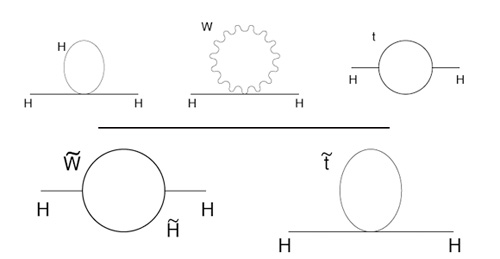
\includegraphics[scale=0.65]{fig/chapt2/higgs_mass_loop.jpg}
\caption{\label{fig:higgs_massloop}The three Feynman diagrams in top row from left to right represent higgs self coupling, W/Z boson and fermion (top quark) coupling respectively, a quantum effects on the Higgs mass. These effects boost the higgs mass to an infinite value which needs to be finite by using some unknown contributions. SUSY suggests supersymmetric partners of the Standard Model particles, one must include additional diagrams, where superpartners cancel out the loops effects in the higgs mass calculation as shown in the lower row. Source of the feynman diagrams is \cite{pub:higgsmassloop}.}
\end{figure}

\subsection{SuperSymmetry}
Supersymmetry (SUSY) is a space-time symmetry relating two different classes of particles, integer spin-0 and spin-1 (bosons) and spin-1/2 (fermions) \cite{phd_thesis:susy}. The SUSY generators $\mathcal{Q}$ transform a fermionic state into a bosonic state and vice–versa
\begin{equation}\label{equ:susy_gen}
\mathcal{Q}|Fermion\rangle = |Boson\rangle, \mathcal{Q}|Boson\rangle = |Fermion\rangle
\end{equation}
When the symmetry is exact, bosons and fermions have the same masses and quantum numbers, except for the spin. But the question arises, why we didn't find the superpartners of the SM particles? For examples electron discovered more than a century ago, if it has a superpartner with same mass and charge with opposite spin, it should to be discovered with simple experiments. Similarly no squark (where "s" stands for superpartner) has been observed in hadron-hadron colliders so for. This suggests that SUSY is not exact symmetry and must be broken in such a way that the superpartners acquire higher masses (higher than the top quark mass) but not too much high to reintroduce the hierarchy problem. This is commonly known as "soft" breaking of the SUSY. Up to now nobody has found a complete satisfactory dynamical way to break SUSY but there are many optional cases where the SUSY can break. One possibility is to introduce the soft term to the SUSY Lagrangian by hand that breaks the SUSY explicitly. 
\begin{equation}\label{equ:soft_break}
\mathcal{L} = \mathcal{L}_{SUSY} + \mathcal{L}_{soft}
\end{equation}
This results a low energy effective SUSY theory and can be used for masses and decays predictions. Minimal Supersymmetric Standard Model (MSSM) is the most economical version that will be discussed in details in the next subsection \ref{subsec:mssm}.   
\subsection{Minimal SuperSymmetric Model}\label{subsec:mssm}
The Minimal Supersymmetric Standard Model (MSSM) \cite{Martin:1997ns} based on the group $SU(3)_{C}\times SU(2)_{L}\times U(1)_{Y}$  with minimal amount of extra fields to the existing one in order to make the theory supersymmetric. In MSSM, each SM particle has its superpartner differ by spin–1/2. An overview of the gauge bosons (spin-1) and their spin–1/2 partners, the gauginos is given in table \ref{table:mssmgauge}. 
\begin{table}[h]%\footnotesize
\centering
     %\begin{tabular}{|p{1.4cm}|p{1.0cm}|p{1.0cm}|}
    \tabulinesep=1.0mm
     \begin{tabu}{|l|c|c|c|c|}
        \hline
        Names & Superfield $\widetilde{S}$ & Spin-$\frac{1}{2}$ & Spin-1 & $SU(3)_{C}$, $SU(2)_{L}$, $U(1)_{Y}$ \\
\hline 
gluino, gluon & $\hat{G}^{a}$ & $\widetilde{G}$ & g & (8, 1, 0) \\ 
\hline
winos, W bosons & $\hat{W}$ & $\widetilde{W}^{\pm}, \quad \widetilde{W}^{0}$ & $W^{\pm}, \quad W^{0}$ & (1, 3, 0) \\ 
\hline
bino, B boson & $\hat{B}$ & $\widetilde{B}^{0}$ & $B^{0}$ & (1, 1, 0) \\
\hline
\end{tabu}
     \caption{Gauge supermultiplets in the MSSM with quantum numbers.\label{table:mssmgauge}}
%\end{center}
\end{table}  
In SM there are three generations of spin-1/2 fermions (quarks and leptons without right handed neutrino) that corresponds to spin-0 SUSY superpartners, squarks and sleptons: $\hat{Q}, \hat{U}_{R}, \hat{D}_{R}, \hat{L}, \hat{E}_{R}$. SUSY requires two Higgs doublets for anomaly cancellation and to give mass to all fermions. Conventionally the two Higgs doublets denoted by $H_{u}$ with Y = +1/2 and $H_{d}$ with Y = -1/2 where the first one gives mass to up-type quarks and the second to the down-type and charged leptons. Table \ref{table:mssmparticles} summarizes particles and their supermultiplets.\\
Unlike the SM, SUSY doesn't respect lepton and baryon number conservation. This can be enforced in a simple way, by introducing a discrete and multiplicative symmetry called R–parity 
\begin{equation}\label{equ:rparity}
R_{p} = (-1)^{2s+3B+L}
\end{equation}
where s, B and L represent spin, baryon and lepton number respectively. For the ordinary particles (fermions, gauge bosons and Higgs bosons), $R_{p}$ = +1 and for their superpartner $R_{p}$ = -1. SUSY allows $R_{p}$ conservative terms in its lagrangian. In practice, R-parity conservation has important effects on the MSSM phenomenology by allowing pair production of the SUSY particles in colliders. Further decay of the SUSY particles comprises odd number of SUSY particles where the stable lightest supersymmetric particle (LSP) is a strong candidate for dark matter if it is neutral and only weakly interacting.    
\begin{table}[h]%\footnotesize
\centering
     %\begin{tabular}{|p{1.4cm}|p{1.0cm}|p{1.0cm}|}
    \tabulinesep=1.0mm
     \begin{tabu}{|l|c|c|c|c|}
        \hline
        Names & Superfield $\widetilde{S}$ & Spin-0 & Spin-$\frac{1}{2}$ & $SU(3)_{C}$, $SU(2)_{L}$, $U(1)_{Y}$ \\
\hline 
squarks, quarks & $\hat{Q}$ & ($\widetilde{u}_{L} \quad \widetilde{d}_{L}$) & ($u_{L} \quad d_{L}$) & (3, 2, $\frac{1}{6}$) \\ 
 
($\times$ 3 families) & $\hat{U}$ & $\widetilde{u}_{R}^{\star}$ & ${u}^{\dagger}_{R}$ & ($\overline{3}$, 1, $-\frac{2}{3}$) \\

                      & $\hat{D}$ & $\widetilde{d}_{R}^{\star}$ & ${d}^{\dagger}_{R}$ & ($\overline{3}$, 1, $\frac{1}{3}$) \\
\hline
sleptons, leptons & $\hat{L}$ & ($\widetilde{\nu} \quad \widetilde{e}_{L}$) & ($\nu \quad e_{L}$) & (1, 2, $-\frac{1}{2}$) \\ 

($\times$ 3 families) & $\hat{E}$ & $\widetilde{e}_{R}^{\star}$ & ${e}^{\dagger}_{R}$ & (1, 1, 1) \\
\hline
Higgs, higgsinos & $\hat{H}_{u}$ & ($H^{+}_{u} \quad H^{0}_{u}$) & ($\widetilde{H}^{+}_{u} \quad \widetilde{H}^{0}_{u}$) & (1, 2, $+\frac{1}{2}$) \\
                 & $\hat{H}_{d}$ & ($H^{0}_{d} \quad H^{-}_{d}$) & ($\widetilde{H}^{0}_{d} \quad \widetilde{H}^{-}_{d}$) & (1, 2, $-\frac{1}{2}$) \\
\hline
\end{tabu}
     \caption{Chiral supermultiplets in the MSSM with quantum numbers.\label{table:mssmparticles}}
%\end{center}
\end{table}  
In light of the above mentioned properties, it is easy to define a globally supersymmetric Lagrangian for MSSM. I will only discuss the final results without going into detail of derivation because it is beyond of the scope of this thesis. The kinetic part of the Lagrangian is the supersymmetric equivalent of the SM and obtained by generalizing the notion of covariant derivative to the SUSY. The   gauge invariant general superpotential, also compatible with renormalizability and R–parity conservation rule, is written as
\begin{equation}\label{equ:mssmpotential}
W = \sum_{i,j=gen}-Y_{ij}^{u}\hat{u}_{Ri}\hat{H}_{2}.\hat{Q}_{j} + Y_{ij}^{d}\hat{d}_{Ri}\hat{H}_{1}.\hat{Q}_{j} + Y_{ij}^{l}\hat{l}_{Ri}\hat{H}_{1}.\hat{L}_{j} + \mu \hat{H}_{2}.\hat{H}_{1}
\end{equation}
where i, j runs over the three generation and $\epsilon_{12}=-\epsilon_{21}=1$ and $\epsilon_{11}=-\epsilon_{22}=0$. $H . Q \equiv \epsilon_{12}H^{1}Q^{2}$ is the SU(2) doublets products and $Y_{ij}^{u,d,l}$ represents the Youkawa couplings among generations. The last term represents a globally supersymmetric mass term for the Higgs doublets.
\subsection{Higgs sector of MSSM}\label{subsec:higgsmssm}
SUSY requires two Higgs doublets for anomaly cancellation and giving mass to all fermions. This minimal version of SUSY is commonly refers as Two Higgs Doublets Model (2HDM). The SM fermions cancels the anomaly by themselves where the superpartner of the Higgs boson is a fermion which contributes to triangle gauge anomalies. The anomaly can be cancelled out by introducing a second fermion which is basically the vector compliment of the first one. Therefore MSSM introduces $H_{u}$ and it's vector compliment $H_{d}$ \cite{Wells:2009kq}. Similarly $\hat{H}_{u}$ is giving mass to up-type quarks and unable to give mass to down-type as in superpotential $\hat{H}_{u}^{*}$ is forbidden and $\hat{H}_{d}$ gives mass to the down-type quarks. The Higgs doublets can be represented in terms of complex field as
\begin{equation}\label{equ:HuHd}
H_{u} = \left(\begin{array}{c}
H^{+}_{u}\\
H^{0}_{u}
\end{array}\right) \quad \textnormal{and} \quad
H_{d} = \left(\begin{array}{c}
H^{0}_{d}\\
H^{-}_{d}
\end{array}\right) 
\end{equation} 
We have not observed the supersymmetric partners of SM particles, which requires the SUSY must be broken at some higher scale. Soft-SUSY breaking mechanism does this job by introducing new terms to the lagrangian in such a way that does not reintroduce quadratic sensitivities to the cutoff. The possibly soft-SUSY terms in the Higgs sector are
\begin{equation}\label{equ:softsusyHiggs}
\mathcal{V}_{1} = m^{2}_{H_{u}} \left( \abs{H^{+}_{u}}^{2} + \abs{H^{0}_{u}}^{2} \right) + 
m^{2}_{H_{d}} \left( \abs{H^{-}_{d}}^{2} + \abs{H^{0}_{d}}^{2} \right) + 
\left\{ b\left(H^{+}_{u}H^{-}_{d} - H^{0}_{u}H^{0}_{d}\right) + h.c  \right\}
\end{equation} 
where the parameters $m^{2}_{H_{u}}$, $m^{2}_{H_{d}}$ and b are arbitrary yet. The total scalar potential is written as \cite{phd_thesis:mssm}
\begin{equation}\label{equ:totallagmssm}
\begin{split}
\mathcal{V} = \left(\abs{\mu}^{2} + m^{2}_{H_{u}}\right) \left( \abs{H^{+}_{u}}^{2} + \abs{H^{0}_{u}}^{2} \right)
+\left(\abs{\mu}^{2} + m^{2}_{H_{d}}\right) \left( \abs{H^{-}_{d}}^{2} + \abs{H^{0}_{d}}^{2} \right)\\
+ \left\{ b\left(H^{+}_{u}H^{-}_{d} - H^{0}_{u}H^{0}_{d}\right) + h.c  \right\} +
\frac{g^{2}}{2}\abs{H^{+*}_{u}H^{0}_{d} + H^{0*}_{u}H^{-}_{d}}^{2}\\
+\frac{g^{2}+g'^{2}}{8}\left( \abs{H^{+}_{u}}^{2} + \abs{H^{0}_{u}}^{2} -  \abs{H^{-}_{d}}^{2} - \abs{H^{0}_{d}}^{2}\right)
\end{split}
\end{equation}
The Higgs mechanism in MSSM can be used to obtain the minimum of this scalar potential in the same way as that in SM where electromagnetism gauge group U(1) is not broken. We have freedom to suppose a vanishing vev for of the electromagnetic part $\big \langle H_{u}^{+} \big \rangle = 0$ at the minimum of the potential where $\left.\frac{\partial \mathcal{V}}{\partial H^{+}_{u}}\right|_{H_{u}^{+}=0} \Rightarrow H_{d}^{-} = 0$. In the same way if we consider $\big \langle H_{u}^{-} \big \rangle = 0, \Rightarrow H_{d}^{+} = 0$. Thus electromagnetism is unbroken, as the charged directions cannot attain a vacuum expectation value. Consider the vev of the neutral part $\big \langle H_{u}^{0} \big \rangle = v_{u}$ and $\big \langle H_{d}^{0} \big \rangle = v_{d}$, hence at minimum of $\mathcal{V}$ we obtain
\begin{equation}
\begin{split}
\left(\abs{\mu}^{2} + m^{2}_{H_{u}}\right)v_{u} = bv_{d} + \frac{g^{2}+g'^{2}}{4}v_{u}\left(v_{d}^{2} - v_{u}^{2}\right)\\
\left(\abs{\mu}^{2} + m^{2}_{H_{d}}\right)v_{d} = bv_{u} - \frac{g^{2}+g'^{2}}{4}v_{d}\left(v_{d}^{2} - v_{u}^{2}\right)\\
\end{split}
\end{equation}
where the vevs values are related to W/Z masses. Consider the kinetic terms for the Higgs field
\begin{equation}
\mathcal{L}_{kin} = \left(D_{\mu}H_{u}\right)^{\dagger} + \left(D^{\mu}H_{u}\right) + \left(D_{\mu}H_{d}\right)^{\dagger} + \left(D^{\mu}H_{d}\right)
\end{equation}
with $D_{\mu} = \partial_{\mu} + ig\tau_{a}W_{\mu}^{a}/2 + ig'yB_{\mu}/2$, the W/Z masses can be written as
\begin{equation}\label{equ:w_zmass_mssm}
\begin{split}
m_{W}^{2} = \frac{g^{2}}{2}\left(v_{u}^{2} + v_{d}^{2}\right)\\
m_{Z}^{2} = \frac{g^{2}+g'^{2}}{2}\left(v_{u}^{2} + v_{d}^{2}\right)
\end{split}
\end{equation}
The two Higgs doublets extension of the MSSM generates eight scalar degrees of freedom (d.o.f) before electroweak symmetry breaking (EWSB). After symmetry breaking three of them eaten by gauge bosons \ref{equ:w_zmass_mssm} and the remaining five d.o.f should manifest as physical states. Among five, two of the d.o.f are charged ($H^{\pm}$), one neutral pseudo scalar ($A^{0}$) and two are neutral $\mathcal{CP}$-even scalar $h^{0}$ and $H^{0}$ states where conventionally $h^{0}$ < $H^{0}$. Their masses can be computed by expanding the doublet fields around their vev $\left( H = \left\langle H \right\langle + \phi + i\varphi \right)$) value and plug this expansion into the Higgs potential. It can be seen that the mass terms of the fields $\varphi_{u}$ and $\varphi_{d}$ only mix among themselves. Taking ratio of vevs of the doublets as $\tan\beta = \frac{v_{u}}{v_{d}}$, we obtain the $\mathcal{CP}$-even $A^{0}$ state:
\begin{equation}
A^{0} = \sqrt{2}\left(\varphi_{u} \cos\beta + \varphi_{d} \sin\beta \right); \quad m^{2}_{A^{0}} = \frac{b}{sin2\beta}
\end{equation}
For $\phi_{u}$ and $\phi_{d}$ we obtain in the same manner the mass terms
\begin{equation}\label{higgs_masses_mssm}
\begin{split}
m_{h^{0}}^{2} = \frac{1}{2}\left[ \left(m_{A^{0}}^{2} + m_{Z}^{2} \right) - \sqrt{(m_{A^{0}}^{2} + m_{Z}^{2})^{2} -4m_{A^{0}}^{2}m_{Z}^{2}\cos^{2}2\beta}\right]\\
m_{H^{0}}^{2} = \frac{1}{2}\left[ \left(m_{A^{0}}^{2} + m_{Z}^{2} \right) + \sqrt{(m_{A^{0}}^{2} + m_{Z}^{2})^{2} -4m_{A^{0}}^{2}m_{Z}^{2}\cos^{2}2\beta}\right]
\end{split}
\end{equation}
Consider the possibility that $m_{A^{0}} \gg m_{Z}$ then mass of the lightest higgs $h^{0}$ is bounded above by $m_{Z}\abs{\cos2\beta}$. One can include higher order corrections and large log resummations that push the Higgs mass to ~ 130 GeV and expected to behave like SM Higgs boson for most of the MSSM parameter space. The discovery of the SM Higgs boson with mass ~ 125 GeV is consistent with these predictions. The corresponding fields for $h^{0}$ and $H^{0}$ are
\begin{equation}
\begin{split}
h^{0} = \sqrt{2}\left(\phi_{u} \cos\alpha - \phi_{d} \sin\alpha \right)\\
H^{0} = \sqrt{2}\left(\phi_{u} \sin\alpha + \phi_{d} \cos\alpha \right)
\end{split}
\end{equation} 
The charged Higgs field is 
\begin{equation}
H^{\pm} = \phi^{\pm}_{d}\sin\beta + \phi^{\pm}_{u}\cos\beta
\end{equation}
We can also obtain the equation
\begin{equation}
\tan\alpha = -\frac{\left[\frac{1}{2}\left(m_{H^{0}}^{2} - m_{h^{0}}^{2}\right)
 + \frac{\cos2\beta}{2}\left(m_{A^{0}}^{2} - m_{Z}^{2}\right) \right]}
 {\frac{1}{2} \left( m_{A^{0}}^{2} + m_{Z}^{2} \right)\sin2\beta}
\end{equation}
In the limit $m_{A^{0}} \gg m_{Z}$, $\tan\beta = -\cot\beta \Rightarrow \alpha\rightarrow \beta - \frac{\pi}{2}$. This limit is commonly known as decoupling limit where the lightest scalar Higgs behave like SM Higgs boson. We use the same condition in calculating k-factor from SusHi generator in \ref{subsec:sushi}. The corresponding tree-level squared Higgs masses are given by \cite{Asner:2013psa}
\begin{equation}\label{equ:alignment_limit}
\begin{split}
m_{h}^{2} \simeq m_{Z}^{2}\cos^{2}2\beta \\
m_{H}^{2} \simeq m_{A}^{2} + m_{Z}^{2}\sin^{2}2\beta \\
m_{H^{\pm}}^{2} \simeq m_{A}^{2} + m_{W}^{2}
\end{split}
\end{equation}
Table~\ref{tab:couplings} gives an overview of the couplings of the neutral 2HDM/MSSM Higgs bosons to up-type quarks, down-type quarks, and vector bosons.
Pseudoscalar decays to vector bosons are forbidden, and the coupling to up-type quarks is inversely proportional to $\tan\beta$, whereas the coupling to down-type quarks is proportional to $\tan\beta$.
\begin{table}[h]
\centering
\begin{tabular}{l c c c}
$\Phi$  & $g_{\Phi \overline{u}u}$ & $g_{\Phi \overline{d}d}$ & $g_{\Phi\mathrm{VV}}$ \\ \hline
h       & $\cos\alpha/\sin\alpha$  & $-\sin\alpha/\cos\beta$  & $\sin(\beta-\alpha)$ \\
H   & $\sin\alpha/\sin\beta$   & $\cos\alpha/\cos\beta$   & $\cos(\beta-\alpha)$ \\
A   & $\cot\beta$              & $\tan\beta$              & 0 \\
\end{tabular}
\caption{Couplings in type-2 2HDM models, in particular also the MSSM, of the three neutral Higgs bosons, denoted as $\Phi$, to up-type quarks, down-type quarks, and vector bosons, in terms of the MSSM parameters $\alpha$ and $\beta$. The couplings are normalised to SM Higgs boson couplings.\label{tab:couplings}}
\end{table}
From the above discussion it can be concluded that in the 2HDM/hMSSM approach we only need two input parameters ($M_{A}, \tan\beta$) to describe the entire MSSM Higgs sector, the Higgs masses and couplings.
\subsection{Heavy Higgs production and decay at LHC}\label{subsec:heavy_H_prod_decay}
In this section I am going to discuss the production and decay of the heavier A, H and H$^{\pm}$ particles at the LHC in the hMSSM/2HDM. I will focus on the high, moderate and low $\tan\beta$ regions as both production and decay are sensitive to $\tan\beta$.\\
\textbf{Neutral Higgs production}:\label{neutral_higgs_prod} 
The dominant production mode for heavy Higgs $\Phi$ = H/A at high energies has leading contribution from two main processes, the gluon fusion mechanism $gg\rightarrow \Phi$, initiated by a heavy quark loop and the associated Higgs production with b quark $gg/q\bar{q}\rightarrow b\bar{b} + \Phi$ or only b quark fusion $b\bar{b}\rightarrow \Phi$ process \cite{Djouadi:2015jea}. The VBF, associated production with massive gauge bosons and top quark pair have low rates as the couplings are highly suppressed or the phase space is not favourable. The production cross sections of both $\mathcal{CP}$-even H and $\mathcal{CP}$-odd A, depend on the magnitude of the Higgs couplings to quarks at tree level but the form factors for the two cases are different as shown in equation \ref{equ:form_factors}. The $\mathcal{CP}$-even lightest state h behaves as SM Higgs in the alignment limit approximation described in \ref{equ:alignment_limit}. In the case of heavy Higgs ($\Phi$ = H/A) the rates are sensitive to the mass, M$_{\Phi}$, and $\tan\beta$ values. The leading order partonic cross sections $\hat{\sigma}$ for the two dominant process $b\bar{b}\rightarrow\Phi$ and $gg\rightarrow\Phi$ can be expressed in terms of partonic c.o.m energy $\hat{s}$ and mass M$_{\Phi}$ as

\begin{equation}
\begin{split}
\hat{\sigma}\left(b\bar{b}\rightarrow\Phi\right) = \frac{\pi}{12}g^{2}_{\Phi bb}\delta\left(\hat{s}-M^{2}_{\Phi}\right)\\
\hat{\sigma}\left(gg\rightarrow\Phi\right) = \frac{G_{F}\alpha^{2}_{s}}{288\sqrt{2}\pi}M^{2}_{\Phi}\delta\left(\hat{s}-M^{2}_{\Phi}\right)\left|\frac{3}{4} \sum\limits_{Q}g_{\Phi QQ}A_{1/2}^{\Phi}\left(\tau_{Q}\right)\right|^{2}
\end{split}
\end{equation}
where the reduce variable is $\tau_{Q} = M_{\Phi}^{2}/4m_{Q}^{2}$ and the quark in loop Q is a heavy bottom or top quark. For consistency I am using the label from reference \cite{Djouadi:2015jea}. The form factors for the two states (H/A) using fermion loops are given by
\begin{equation}\label{equ:form_factors}
\begin{split}
A^{H}_{1/2}\left(\tau\right) = 2\left[\tau+\left(\tau-1\right)f\left(\tau\right)\right]\tau^{-2}\\
A^{A}_{1/2}\left(\tau\right) = 2\tau^{-1}f\left(\tau\right)
\end{split}
\end{equation} 
In case of top quarks in the loop, the reduce variable $\tau_{t} = M_{\Phi}^{2}/4m_{t}^{2} \approx 4$ at $M_{\Phi}=750$ GeV and $m_{t}=172$ GeV makes the form factors $\left|A^{A}_{1/2}\left(\tau\right)/H^{A}_{1/2}\left(\tau\right)\right|^{2} \sim 2$ that increases the $\mathcal{CP}$-odd cross section two times compare to the $\mathcal{CP}$-even state \cite{Djouadi:2016eyy}.
\begin{equation}
\frac{\sigma\left(gg\rightarrow A\right)}{\sigma\left(gg\rightarrow H\right)}\approx 2
\end{equation}
As stated above, the production rate is sensitive to the $\tan\beta$ values. At low $\tan\beta$ the phenomenology is more richer for heavy Higgs (H/A) production. In this limit, coupling to the top quark, $g_{\Phi t\bar{t}} \propto 1/\tan\beta$, increases drastically and the dominant contribution to the cross section coming from the gluon fusion process $gg\rightarrow \Phi$ via top quark loops. On the other hand, contribution from $b\bar{b}\rightarrow \Phi$ is negligible to cross sections as the coupling, $g_{\Phi b\bar{b}}$, is very small. For higher mass, M$_{\Phi} \geq 2m_{t}$, the associated production with $t\bar{t}$ and massive gauge boson is suppressed because of the small phase-space and negligible coupling $g_{HVV}$. The $\mathcal{CP}$-invariance forbids $AVV$ couplings as a result the $\mathcal{CP}$-odd state is not produced. \\
In case of intermediate value of $\tan\beta \approx 3-10$, both the couplings $g_{\Phi b\bar{b}}$ and $g_{\Phi t\bar{t}}$ have its minimum level hence results a smaller production cross section. For $\tan\beta \approx \sqrt{m_{t}/\bar{m}_{b}} \approx 7$ the cross section has its minimum value where top quarks mass $m_{t}$ = 173 GeV and b-quark mass $\bar{m}_{b}\approx 3$ in the $\overline{MS}$ scheme \cite{Baglio:2015wcg}. \\
For high values of $\tan\beta \geq 10$, the top quark couplings $g_{\Phi t\bar{t}}$ decreases to a large scale while the b-quark couplings $g_{\Phi b\bar{b}}$ enhanced which dominates the b-quark contribution in the $gg\rightarrow \Phi$ loop. The production rates for both processes $gg\rightarrow \Phi$ and $b\bar{b}\rightarrow \Phi$ are the same but at $M_{\Phi} \gtrsim 2m_{Q}$, $gg\rightarrow \Phi$ is known to NLO while $b\bar{b}\rightarrow \Phi$ in known to NNLO corrections \cite{Harlander:2003ai}. But for top quark loop we don't include the NNLO corrections as it is only valid for $M_{\Phi} \lesssim 2m_{Q}$ \cite{Dittmaier:2011ti}. Figure \ref{fig:Heavy_H_prod_xsec}a shows production cross sections for $\mathcal{CP}$-even and odd states at c.o.m energy 14 TeV and $\tan\beta$ = 2.5 exploiting the mass of the SM higgs to be 126 GeV. At M$_{\Phi} \approx 2m_{t}$ there is a sharp increase in cross sections especially for $CP$-odd state A.     
\\
\textbf{Charged Higgs production}:
The couplings of charged Higgs (H$^{\pm}$) is proportional to up and down-type quarks by the following relation
\begin{equation}\label{equ:charge_higgs}
g_{H^{\pm}\bar{u}d} \propto m_{d}\tan\beta\left(1+\gamma_{5}\right) + m_{d}\cot\beta\left(1-\gamma_{5}\right)
\end{equation} 
The second part of \ref{equ:charge_higgs} has large contribution at low $\tan\beta$ values because of the heavy top quark. At very high $\tan\beta$, contribution from the first part ($\propto m_{d}\tan\beta$) increases and the second part suppressed. This shows a similar behaviour as described for neutral heavy Higgs section above. When the mass of charged Higgs in less than the top mass, M$_{H^{\pm}} \lesssim 160$ GeV, it is produced in the decay of one top quark ($t\rightarrow bH^{+}$) in the process $gg + q\bar{q}\rightarrow t\bar{t}$ at LHC. Figure \ref{fig:Heavy_H_prod_xsec}b shows M$_{H^{\pm}}$ versus cross section for $\tan\beta$ = 1, 3, 10, 15, 35, 60 at $\sqrt{s} = 14$ TeV where the dominant contribution is coming from the lowest $\tan\beta$ values. More information about this plot can be found in this reference \cite{Djouadi:2015jea}.

\begin{figure}[htp]
\centering
\begin{tabular}{cc}
\hspace{0.3cm}
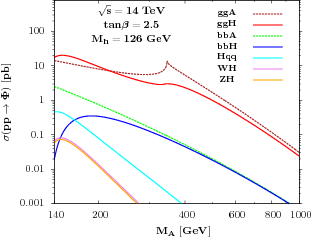
\includegraphics[scale=0.61]{fig/chapt2/Heavy_higgs_prod_xsec.png}
& \hspace{-0.3cm} 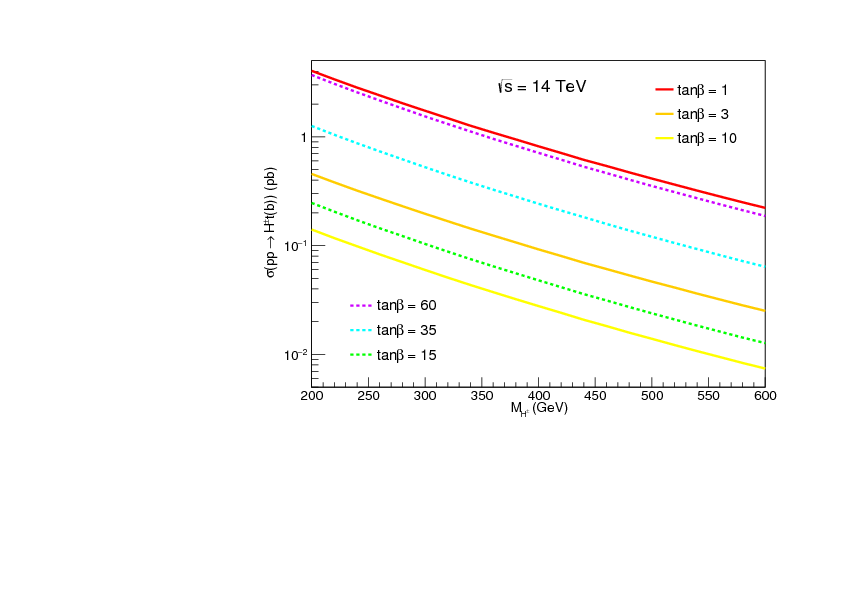
\includegraphics[trim={8cm 6.0cm 0 0},clip, scale=0.4]{fig/chapt2/plots_xs_Htb_14TeV.png}\\
  \qquad\qquad\qquad\qquad ($\mathbf{a}$)\qquad\qquad\qquad&($\mathbf{b}$)\\
\end{tabular}
\caption{(a): Heavy Higgs (neutral) boson production cross sections in MSSM for main channels with $\tan\beta$ = 2.5 and SM Higgs mass is 126 at $\sqrt{s} = 14 TeV$ w.r.t M$_{A}$. (b): Charged Higgs production cross sections for a range of $\tan\beta$ values w.r.t to M$_{H^{\pm}}$ \cite{Djouadi:2013vqa,Djouadi:2015jea}. }\label{fig:Heavy_H_prod_xsec}
\end{figure}
\noindent\textbf{Neutral Higgs decay}: The decay of neutral Higgs ($\Phi$ = H/A) is dictated by $\tan\beta$ value in a similar pattern as in production because of coupling sensitivity to $\tan\beta$. In decoupling limits ($\sin\left(\alpha-\beta\right) = 1$), the couplings of $\mathcal{CP}$-even state ($\cos\alpha/\cos\beta$) \ref{tab:couplings} explicitly equal to $\tan\beta$. For high $\tan\beta \gtrsim 10$, the couplings to b-quark and tau lepton enhanced and it decays exclusively to a $b\bar{b}$ or $\tau^{+}\tau^{-}$ pairs with branching ratios BR($\Phi\rightarrow b\bar{b} \approx 90\%$) and BR($\Phi\rightarrow \tau^{+}\tau^{-} \approx 10\%$) respectively. Decay to $t\bar{t}$ pair is highly suppressed for high $\tan\beta$ range as g$_{\Phi t\bar{t}} \propto 1/\tan\beta$. Other decay modes of $\mathcal{CP}$-even state H like in di-boson ($H\rightarrow VV; V= WW, ZZ$) and decay of $\mathcal{CP}$-odd state into lighter Higgs and Z bosons are strongly suppressed in the alignment limit approximation. For $H\rightarrow hh$ in the limit $M_{H}\gtrsim 2M_{h}$, the coupling $g_{Hhh}$ vanished at high $\tan\beta$ \cite{Baglio:2015wcg} 
\begin{equation}
g_{Hhh} = 2\sin2\alpha \sin\left(\alpha+\beta\right)-\cos2\alpha\cos\left(\alpha+\beta\right)+3\frac{\Delta M^{2}_{22}}{M^{2}_{Z}}\frac{\sin\alpha}{\sin\beta}\cos\alpha^{2}
\end{equation}
becomes
\begin{equation}
\begin{split}
g_{Hhh} \xrightarrow{\text{M}_{A}\gg \text{M}_{z}} -3\Delta \frac{M^{2}_{22}}{M_{Z}^{2}}\times \sin2\beta\\
\sin2\beta \propto \cot\beta \xrightarrow{\tan\beta \gtrsim 10} 0
\end{split} 
\end{equation}  
For $\Phi\rightarrow \gamma\gamma$ channel, the coupling is very small and shows a constant behaviour for $0.3\lesssim \tan\beta \lesssim 10$ which reduces abruptly for $\tan\beta \gtrsim 10$. Same pattern is followed by $\Phi \rightarrow gg$ channel but higher coupling compare to $\Phi\rightarrow \gamma\gamma$. For intermediate values of $\tan\beta \approx 5-10$ with M$_{\Phi} < 2m_{t}$, the bosonic decay of $H\rightarrow WW, ZZ$ has significant contribution as it's competition is only with the $H\rightarrow b\bar{b}$ decay. In this limit the $H\rightarrow t\bar{t}$ decay is suppressed as the phase-space is not feasible. At $\tan\beta$ = 2.5 and $2M_{h} \lesssim M_{\Phi}< 2m_{t}$, $H\rightarrow hh$ and $A\rightarrow hZ$ have prominent branching ratios. Figure \ref{fig:Heavy_H750_BR} shows branching ratios w.r.t $\tan\beta$ for a specific M$_{\Phi}$ = 750 GeV. Figure \ref{fig:Heavy_Hpm_BR}a and b show mass versus branching ratios for $\mathcal{CP}$-odd and $\mathcal{CP}$-even states for $\tan\beta$ = 2.5 and M$_{h}$ = 126 GeV. 
\begin{figure}[htp]
\centering
\hspace{-0.3cm} 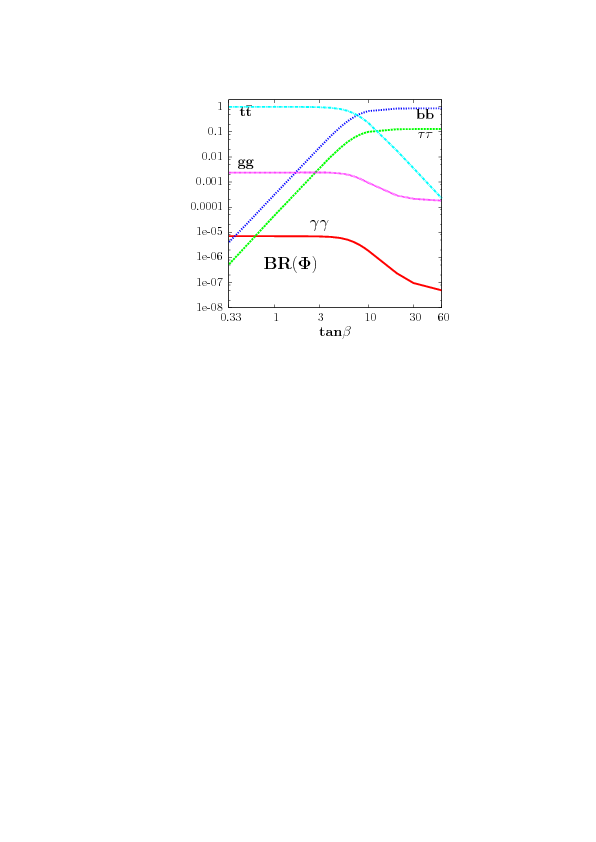
\includegraphics[trim={6cm 17.50cm 4.0cm 3.50cm},clip, scale=0.8]{fig/chapt2/BR-Atb.png}
\caption{The branching ratios of $\Phi$ = H/A in different channels as a function of $\tan\beta$ exploiting the M$_{\Phi}$ = 750 GeV \cite{Djouadi:2016eyy}. }\label{fig:Heavy_H750_BR}
\end{figure}
\\
\noindent \textbf{Charged Higgs decay}:
In high range of $\tan\beta \gtrsim 10$ with M$_{H^{\pm}} \lesssim m_{t} - m_{b}$, the dominant decay of H$^{\pm}$ occurs in the $H^{\pm}\rightarrow \tau\nu$ channel with a small fraction in hadronic decay mode. For high mass range,  M$_{H^{\pm}} > m_{t} - m_{b}$, the decay channel M$_{H^{\pm}} \rightarrow tb$ becomes the dominant one while $H^{\pm}\rightarrow \tau\nu$ branching ratio suppressed. A same saw pattern for the mentioned mass range is followed for low $\tan\beta$ by these two channels but this time the $H^{\pm}\rightarrow \tau\nu$ channel suppressed more compare to high $\tan\beta$. For low $\tan\beta$ and M$_{H^{\pm}} \gtrsim 160 $ GeV, another important channel, $H^{\pm}\rightarrow hW^{\pm}$, comes into play with smaller branching ratio than the $H^{\pm}\rightarrow tb$ one. Figure \ref{fig:Heavy_Hpm_BR}c shows branching ratios at a function of M$_{H^{\pm}}$ for H$^{\pm}$ at $\tan\beta$ = 2.5. Until now I discussed all the main decay channels for neutral and charged heavy higgs in different $\tan\beta$ ranges but there are many more with small contributions. To complete the picture, I write all of them in the form of total decay width equations. The total decay widths of neutral and charged Higgs are given in \ref{equ:neutral_decay_widths} and \ref{equ:charged_decay_widths} respectively. For completeness I mentioned the SUSY decay widths in the formulae. FH is abbreviation for $\mathtt{FEYNHIGGS}$ and HD stands for $\mathtt{HDECAY}$ programs commonly used for decay widths and branching ratio calculation of the Higgs boson with more detail is given here \cite{Dittmaier:2012vm}.
\begin{equation}\label{equ:neutral_decay_widths}
\begin{split}
\Gamma_{\Phi} = \Gamma^{\text{FH}}_{\Phi \rightarrow\tau^{+}\tau^{-}} + \Gamma^{\text{FH}}_{\Phi \rightarrow\mu^{+}\mu^{-}} + \Gamma^{\text{FH/P4f}}_{\Phi \rightarrow \text{W}^{*}\text{W}^{*}} + \Gamma^{\text{FH/P4f}}_{\Phi \rightarrow \text{Z}^{*}\text{Z}^{*}}\\
+ \Gamma^{\text{HD}}_{\Phi \rightarrow b\bar{b}} + \Gamma^{\text{HD}}_{\Phi \rightarrow t\bar{t}} + \Gamma^{\text{HD}}_{\Phi \rightarrow c\bar{c}} + \Gamma^{\text{HD}}_{\Phi \rightarrow gg} + \Gamma^{\text{HD}}_{\Phi \rightarrow \gamma \gamma} + \Gamma^{\text{HD}}_{\Phi \rightarrow \text{Z} \gamma}\\
+ \Gamma^{\text{FH}}_{\Phi \rightarrow \text{Zh}} + \Gamma^{\text{FH}}_{\Phi \rightarrow \text{hh}} + \Gamma^{\text{FH}}_{\Phi \rightarrow \text{ZA}} + \Gamma^{\text{FH}}_{\Phi \rightarrow \text{AA}}  + \Gamma^{\text{HD}}_{\Phi \rightarrow \text{H}^{\pm}\text{W}^{\mp}} + \Gamma^{\text{FH}}_{\Phi \rightarrow \text{SUSY}}
\end{split}
\end{equation}
\begin{equation}\label{equ:charged_decay_widths}
\begin{split}
\Gamma_{\text{H}^{\pm}} = \Gamma^{\text{FH}}_{\text{H}^{\pm} \rightarrow\tau\nu_{\tau}} + \Gamma^{\text{FH}}_{\text{H}^{\pm} \rightarrow\mu\nu_{\mu}} + \Gamma^{\text{FH}}_{\text{H}^{\pm} \rightarrow \text{hW}} + \Gamma^{\text{FH}}_{\text{H}^{\pm} \rightarrow \text{HW}} + \Gamma^{\text{FH}}_{\text{H}^{\pm} \rightarrow \text{AW}}\\
+ \Gamma^{\text{HD}}_{\text{H}^{\pm} \rightarrow \text{tb}} + \Gamma^{\text{HD}}_{\text{H}^{\pm} \rightarrow \text{ts}} + \Gamma^{\text{HD}}_{\text{H}^{\pm} \rightarrow \text{td}} +  \Gamma^{\text{HD}}_{\text{H}^{\pm} \rightarrow \text{cb}} + \Gamma^{\text{HD}}_{\text{H}^{\pm} \rightarrow \text{cs}} + \Gamma^{\text{HD}}_{\text{H}^{\pm} \rightarrow \text{cd}}\\
+ \Gamma^{\text{HD}}_{\text{H}^{\pm} \rightarrow \text{ub}} + \Gamma^{\text{HD}}_{\text{H}^{\pm} \rightarrow \text{us}} + \Gamma^{\text{HD}}_{\text{H}^{\pm} \rightarrow \text{ud}} + \Gamma^{\text{HD}}_{\text{H}^{\pm} \rightarrow \text{SUSY}}
\end{split}
\end{equation}
\begin{figure}[htp]
\centering
\begin{tabular}{ccc}
\hspace{-0.7cm}
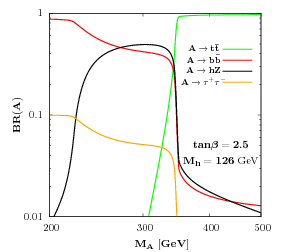
\includegraphics[scale=0.47]{fig/chapt2/A_br.png}
& \hspace{-0.65cm} 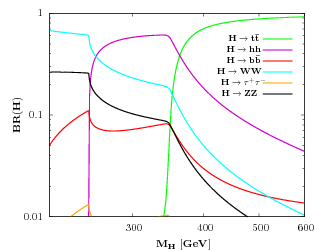
\includegraphics[scale=0.47]{fig/chapt2/H_br.png}
& \hspace{-0.65cm} 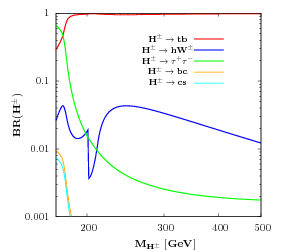
\includegraphics[scale=0.47]{fig/chapt2/H_pm_br.png}\\
  \qquad ($\mathbf{a}$)\qquad\qquad&($\mathbf{b}$)\qquad\qquad&($\mathbf{c}$)\\
\end{tabular}
\caption{Heavy Higgs decay branching ratios in MSSM, (a) pseudo scalar Higgs A, (b) Scalar Higgs H and (c) charged Higgs (H$^{\pm}$) with $\tan\beta$ = 2.5 and SM Higgs mass is 126. Plot are taken from \cite{Djouadi:2013vqa}. }\label{fig:Heavy_Hpm_BR}
\end{figure}
\noindent \subsection{The $\Phi \rightarrow t\bar{t}$ channel with interference from SM $gg \rightarrow t\bar{t}$}
\textbf{Introduction to interference:} In particle physics a process is represented by one or more Feynman diagrams and the resultant amplitude is expressed in terms of matrix element. For a given process, interference is the contribution from the cross terms of different processes to the final amplitude which introduces a peak, dip, nothingness or more complex peak-dip or dip-peak structure. It can be considered a similar phenomenon as quantum wave interference. Interference depends on physics model and it effects different kinematics of the searched particle in different ways. Most of particles discoveries are carried out by simply confirming a resonant peak in the transverse invariant mass distribution above the continuum backgrounds, like $J/\Psi$ meson, $W/Z$ bosons, higgs ($h$) boson and top quark. Currently most of LHC new physics searches focus on the same search strategy by looking to the access above the continuum background. But in some cases the kinematics (mass, $p_{T}$) of the searching particle are not pure Breit-Wigner (BW) resonance peak but instead a modified shape from the interfering background or other resonance. The complicated dip-peak or peak-dip structure is more sensitive to new physics than the simple resonant peak. It was first realised in the $gg\rightarrow\Phi\rightarrow t\bar{t}$ channel \cite{Gaemers:1984}. This channel along with interference effect is studied in this thesis and will be explained in detail after the general introduction to the interference. \\
\noindent Consider a two body scattering $ab\rightarrow {cd}$ whose partonic differential cross section w.r.t angular variable $z\cos\theta^{*}$, where $\theta^{*}$ is the scattering angle in the c.o.m frame, can be expressed as \cite{Jung:2015gta}   
\begin{equation}\label{equ:gen_interference}
\frac{d\hat{\sigma}}{dz}=\frac{1}{32\pi\hat{s}}\sum \left| \mathcal{A}_{\text{bg}}e^{i\phi_{\text{bg}}}+\frac{M^{2}}{\hat{s}-M^{2}+iM\Gamma}.\mathcal{A}_{\text{res}}e^{i\phi_{\text{res}}} \right|^{2}.
\end{equation}
In equation \ref{equ:gen_interference} the sum is for all spin and color components, $\hat{s}$ is the partonic energy and $\phi_{bg,res}$ is the complex phase of background and resonant part respectively. $\mathcal{A}_{bg}$ shows the continuum background amplitude and the term $\mathcal{A}_{res}$ is resonance amplitude for the searching particle with mass A and width $\Gamma$. Expanding the square and re-arranging, we get equation \ref{equ:split_inter} where we define new terms, $\sigma_{int}$, R, $\omega$ and $\phi = \phi_{res}-\phi_{bg}$ with definitions in equation \ref{equ:inter_variables}.  

\begin{equation}\label{equ:split_inter}
\hat{\sigma}=\hat{\sigma}_{\text{bg}}+\frac{M^{4}}{\left(\hat{s}-M^{2}\right)^{2}+M^{4}\omega^{2}}\times\left[\frac{2\left(\hat{s}-M^{2}\right)}{M^{2}}\hat{\sigma}_{\text{int}}c_{\phi}+\hat{\sigma}_{\text{res}}\left(1+\frac{2\omega}{R}s_{\phi} \right) \right]
\end{equation}
where c$_{\phi}$ = cosine$\phi$ and s$_{\phi}$ = sine$\phi$.
\begin{equation}\label{equ:inter_variables}
\begin{split}
\hat{\sigma}_{\text{bg,res}}=\frac{1}{32\pi\hat{s}}\int dz \sum \mathcal{A}^{2}_{\text{bg,res}},\\
\hat{\sigma}_{\text{int}}e^{i\phi}=\frac{1}{32\pi\hat{s}}\int dz \sum \mathcal{A}_{\text{bg}}\mathcal{A}_{\text{res}}e^{i\left(\phi_{\text{res}}-\phi_{\text{bg}}\right)},\\
R=\frac{\hat{\sigma}_{\text{res}}}{\hat{\sigma}_{\text{int}}},\qquad \omega \equiv \frac{\Gamma}{M}.
\end{split}
\end{equation}
\noindent $\omega$, R and  $\phi$ are parameters of interest with the later two are respectively relative strength and phase difference between signal resonance and background continuum. The second interference term in equation \ref{equ:split_inter} further consists of two parts, the real with $\text{c}_{\phi}$ and imaginary s$_{\phi}$, decides the final interference pattern. The well known peak-dip or dip-peak structure arises from the real interference part with s$_{\phi}$ = 0 with a final shift in the resonance peak position. We are focusing on the pure resonance as well as peak-dip structure of the signal in this analysis. The imaginary term makes the shape more interesting at specific conditions of $\phi$ and factor C where C is defined as
\begin{equation}\label{equ:correction_term}
C \equiv \left(1+\frac{2\omega}{R}s_{\phi} \right).
\end{equation} 
At $\phi=-\pi /2$ and C < 0, the $gg\rightarrow\Phi\rightarrow AB$ line adopted a pure dip shape shown in figure \ref{fig:dip_peak_nothing_H_A}a by the green line. On contrary, the access can be achieved by C > 0 shown by the orange line in figure \ref{fig:dip_peak_nothing_H_A}a where its amplitude can be increased or decreased relative to pure resonance (dashed-orange line) by varying the value of $\phi$. At $\phi=-\pi /2$ and C = 0, the line shape becomes more interesting when both the real and imaginary part disappear and the signal line now running parallel with continuum background. These types of shapes are termed as "nothingness" and need more careful treatment. All the above defined signal structures demand a new search strategy compare to what we are searching for simple resonance. 

\begin{figure}[htp]
\centering
\begin{tabular}{cc}
\hspace{-0.3cm}
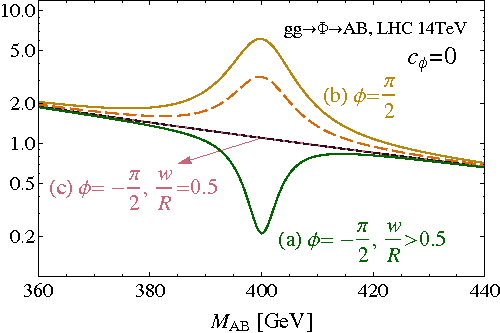
\includegraphics[scale=0.41]{fig/chapt2/dip_peak_nothing.png}
& \hspace{-0.45cm} 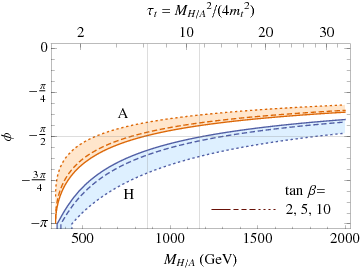
\includegraphics[scale=0.61]{fig/chapt2/fig_phase_A_H.png}\\
  \qquad\qquad\qquad ($\mathbf{a}$)\qquad\qquad\qquad\qquad&($\mathbf{b}$) \\
\end{tabular}
\caption{(a): Resonance shapes after pure imaginary interference (c$_{\phi}$ = 0) with mass = 400 GeV, $\Gamma$ = 10 GeV and R = 0.035. Green line is pure dip, orange is access, orange-dashed is pure resonance, red is nothingness and solid black is continuum background. Arbirary units are used on y-axis. (b): shows the relative phase $\phi$ between continuum $gg\rightarrow t\bar{t}$ and resonace $gg\rightarrow \Phi \rightarrow t\bar{t}$ w.r.t M$_{H/A}$ at different $tan\beta$ values (2, 5, 10) with $\tau_{t} = M^{2}_{H/A}/(4m_{t}^{2})$ at the upper horizental axis. For all values of $tan\beta$, the $-\pi/2$ condition achieved by $\mathcal{CP}-$odd state ($A$) much faster than the $\mathcal{CP}-$even state ($H$) shown by vertical lines \cite{Jung:2015gta}. }\label{fig:dip_peak_nothing_H_A}
\end{figure}

\begin{figure}[htp]
\centering
\begin{tabular}{cc}
\hspace{-0.3cm}
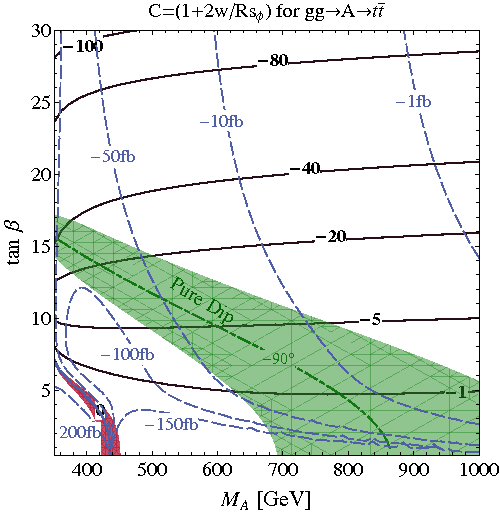
\includegraphics[scale=0.42]{fig/chapt2/nwafix-ttbar-A.png}
& \hspace{-0.4cm} 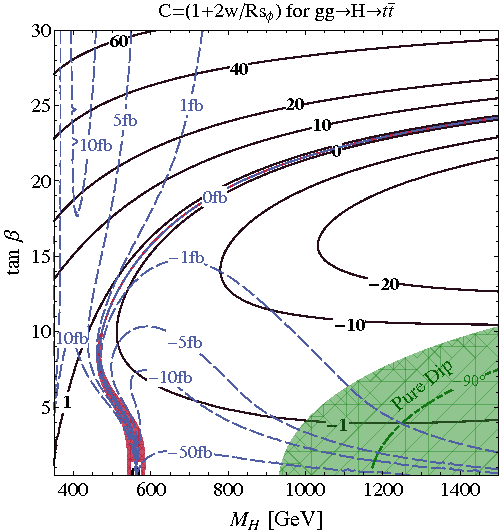
\includegraphics[scale=0.4]{fig/chapt2/nwafix-ttbar-H.png}\\
  \qquad ($\mathbf{a}$)\qquad\qquad&($\mathbf{b}$) \\
\end{tabular}
\caption{ \cite{}. }\label{fig:NWA_H_A}
\end{figure}


The correlation resulting from projecting the spin of $t$ onto the spin of \cite{Berge:2008dr, PhysRevD.58.114031}
\begin{equation}
\left\langle S \right\rangle = \frac{a_{1}^{2}-3a_{2}^{2}}{4a_{1}^{2}+4a_{2}^{2}}
\end{equation}\label{equ:tt_spin}
\begin{figure}[htbp]
\centering
%\hspace{2.0cm}
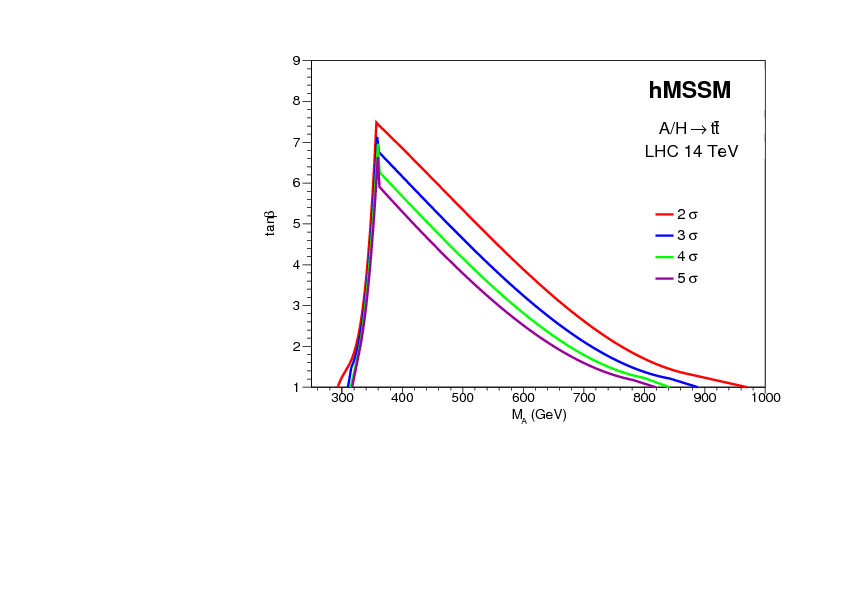
\includegraphics[trim={8cm 6.0cm 0 0},clip, scale=0.6]{fig/chapt2/plots_constraints_LHC14_300_AH_tt.png}
\caption{Sensitivity levels for $\Phi\rightarrow t\bar{t}$ channel at $\sqrt{s}=14$ TeV with total integrated luminosity $\mathcal{L}=300 \text{f}\text{b}^{-1}$ in hMSSM and ($\tan\beta, \text{M}_{A}$) plane. At M$_{\Phi} \approx 2\text{m}_{t}$, we have a large $\tan\beta$ space upto 7.5 which shows the sensitivity of the top quark to new physics \cite{Djouadi:2015jea}. }\label{fig:Htt_sensitivity}
\end{figure}


\begin{figure}[htp]
\centering
\begin{tabular}{cc}
\hspace{-0.3cm}
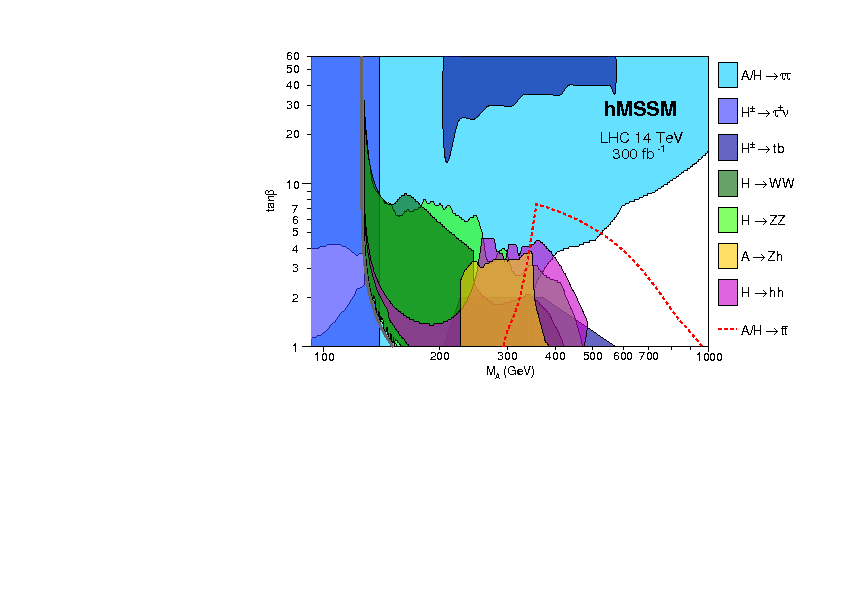
\includegraphics[trim={8cm 6.0cm 0 0},clip, scale=0.4]{fig/chapt2/httplots_constraints_LHC14_300fb_all.png}
& \hspace{-2.4cm} 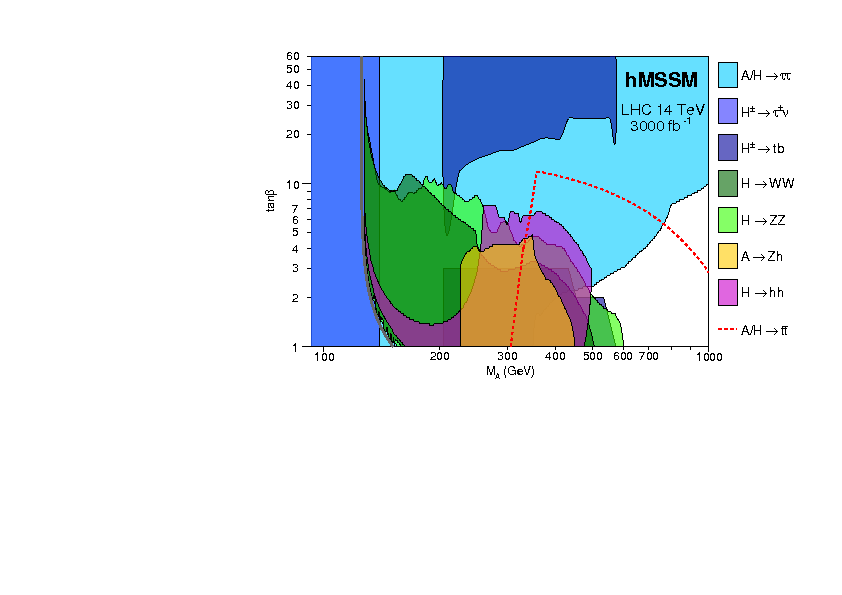
\includegraphics[trim={8cm 6.0cm 0 0},clip, scale=0.4]{fig/chapt2/httplots_constraints_LHC14_3000fb_all.png}\\
  \qquad ($\mathbf{a}$)\qquad\qquad&($\mathbf{b}$)\qquad\qquad\qquad\qquad \\
\end{tabular}
\caption{All decay channels of neutral and charged Higgs with expectation of 2$\sigma$ at $\sqrt{s}=14$ TeV using hMSSM with total integrated luminosity $\mathcal{L}=300 \text{f}\text{b}^{-1}$ (a) and  HL-LHC $\mathcal{L}=3000 \text{f}\text{b}^{-1}$ (b) using hMSSM and ($\tan\beta, \text{M}_{A}$) plane. The red-dashed contour shows the $\Phi\rightarrow t\bar{t}$ channel where it's sensitivity lies in low $\tan\beta$ and high mass region \cite{Djouadi:2015jea}. }\label{fig:Heavy}
\end{figure}
   
\clearpage{\pagestyle{empty}\cleardoublepage}

\graphicspath{{chapt_dutch/}{intro/}{chapt2/}{chapt3/}{chapt4/}{chapt5/}{chapt6/}{chapt7/}{chapt8/}}
%\usepackage{zref-xr}

% Header
\renewcommand\evenpagerightmark{{\scshape\small Chapter 3}}
\renewcommand\oddpageleftmark{{\scshape\small LHC and the CMS Experiment}}

\renewcommand{\bibname}{References}

\hyphenation{}

\chapter[LHC and the CMS Experiment]%
{LHC and the CMS detector}
\label{chap:2}

\section{The Large Hadron Collider at CERN}
\label{sec:lhc}
The Large Hadron Collider (LHC) is a circular protons and heavy ions collider with a circumference of ~27 km, 100 m underground, operated at the laboratories of the European Organization for Nuclear Research (CERN\footnote{Called Conseil Européen pour la Recherche Nucléaire.}) in Geneva, Switzerland \cite{Bruning:lhc}. LHC has designed to operate at centre of mass (CoM) energy $\sqrt{s}$ = 14 TeV which makes it the world's most powerful accelerator. Proton-proton (pp) collision is the main part of the LHC physics program where part of the machine schedule is periodically dedicated to the delivery of heavy-ion collisions. The accelerator complex at CERN is a succession of machines to accelerate particles beams in many steps before injecting into the main ring. Protons are first accelerated in different linear accelerators (LINAC) to the energy of 50 MeV. The beam is then injected into the Proton Synchrotron Booster (PSB) followed by the Proton Synchrotron (PS), which pushes the beam to 25 GeV. Protons are then sent to the Super Proton Synchrotron (SPS) where they are accelerated to 450 GeV. Most of the pre-accelerators in the chain have their own experimental halls where beams are used for different purposes such as other particle-physics experiments, test beams or irradiation of detector material for radiation-hardness studies.\\
The protons beams are finally transferred to the largest ring of the LHC to attain 6.5 TeV energy per beam. It includes two adjacent beam pipes, each containing one of two colliding beams, which travel in opposite directions in the collider ring. Ultrahigh beam vacuum ($10^{10}$ Torr) is created to avoid possible collision with gas molecules. The beams are guided and focused in circular trajectory by using superconducting (1.9-4 K) dipole and quadrupole magnets. In the LHC, beams are accelerated/decelerated by the electromagnetic field generated by radio-frequency (RF) cavities (eight per beam) located along the collider ring: each of these cavities also operates in superconducting state, at a temperature of approximately 4.5 K, and can deliver a voltage of 2 MV at a frequency of 400 MHz. The main role of the RF cavities is to keep the 2808 proton bunches tightly bunched to ensure high luminosity at the collision points and hence maximize the number of collisions (luminosity). The two beams are crossing each other at four interaction points where detectors installed. The CERN accelerator complex with four interaction points is shown in Fig.\ref{fig:LHC_complex}.\\

\begin{figure}[h]
\centering
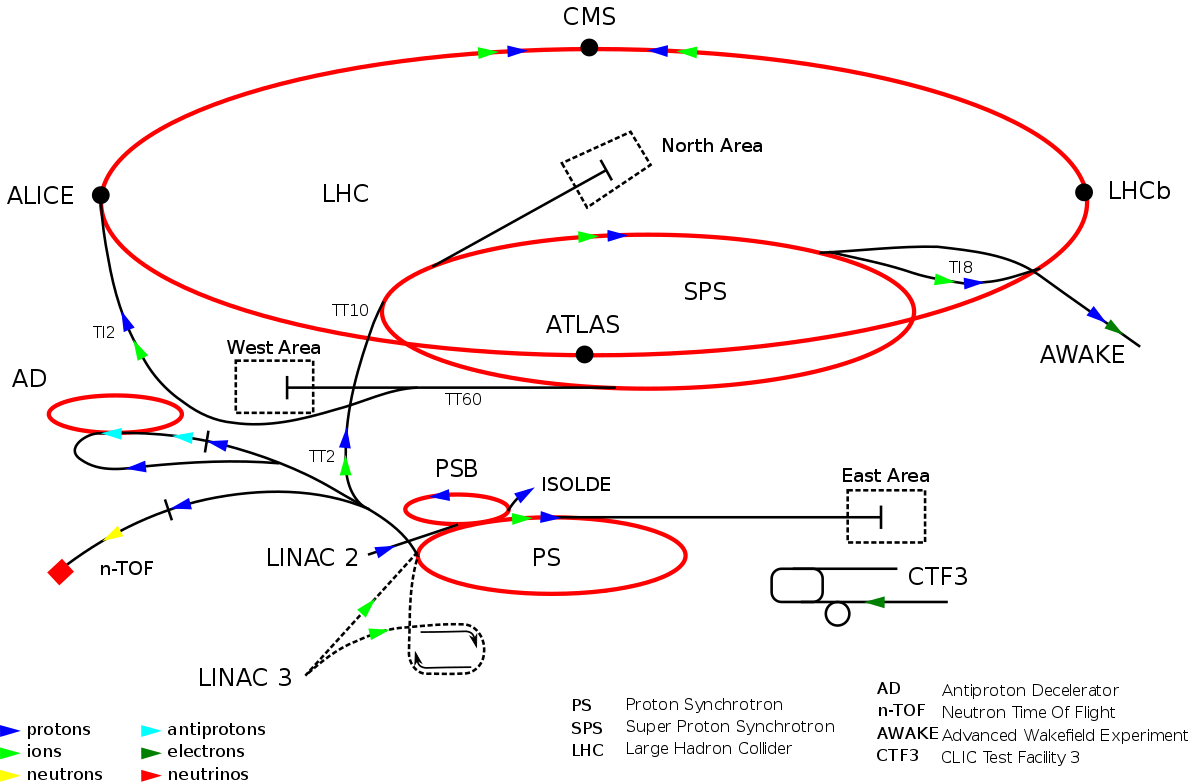
\includegraphics[width=0.9\textwidth]{fig/chapt3/LHC_complex.png}
\caption{\label{fig:LHC_complex} The CERN accelerator complex. The proton injection chain for the LHC
starts from the LINAC2 and proceeds through the Booster, PS and SPS.}
\end{figure}

The performance of an accelerator is measured in terms of instantaneous luminosity $\mathcal{L}$, the most important characteristic of a collider is, that ties event rate to the cross-section ($\sigma$) of a process:
\begin{equation}
\frac{dN_{i}}{dt} = \sigma_{i} \mathcal{L}(t)
\end{equation}
Where i indicates any general process and $\mathcal{L}(t)$ is the instantaneous luminosity that depends on the number of interaction per unit time. The machine instantaneous luminosity related to the beam parameters, and can be written as:
\begin{equation}
\mathcal{L} = \frac{f_{rel}N_{b}^{2}n_{b}\gamma_{r}}{4\pi\epsilon_{n}\beta^{\ast}}F
\end{equation}
where $f_{rev}$ = 11 kHz is the revolution frequency, $N_{b}$ is the number of particles per bunch, $n_{b}$ is the number of bunches per beam, $\epsilon_{n}$ is the normalized transverse beam emittance, $\beta^{\ast}$ is the beta function at the collision point, which measures the beam focalization and is corrected by the relativistic gamma factor $\gamma_{r}$, and F is a geometric luminosity reduction factor that accounts for the crossing angle at the interaction point \cite{lumi_formula}. The amount of data delivered by a collider is measured in terms of total integrated luminosity $L = \int\mathcal{L}dt$ and measured in unit fb$^{-1}$. Since discoveries in particle physics depends on statistics, the higher luminosity, the more chances physicists have to discover a particle or process.\\
During 2016, the LHC has operated at CoM energy $\sqrt{s} = 13$ TeV with a bunch spacing of 25 ns. Reducing the $\beta^{\ast}$ parameter from 80 cm to 40 cm, the the nominal LHC luminosity crossed the record value $10^{34}$ cm$^{-2}$ s$^{-1}$ in late summer 2016. The instantaneous luminosity delivered by LHC (blue) and recorded by CMS (yellow) is shown in \ref{fig:cms_lumi}(a) and the total integrated luminosity is in \ref{fig:cms_lumi}(b) during 2016.   


\begin{figure}[htp]
\centering
\begin{tabular}{cc}
\hspace{-0.3cm}
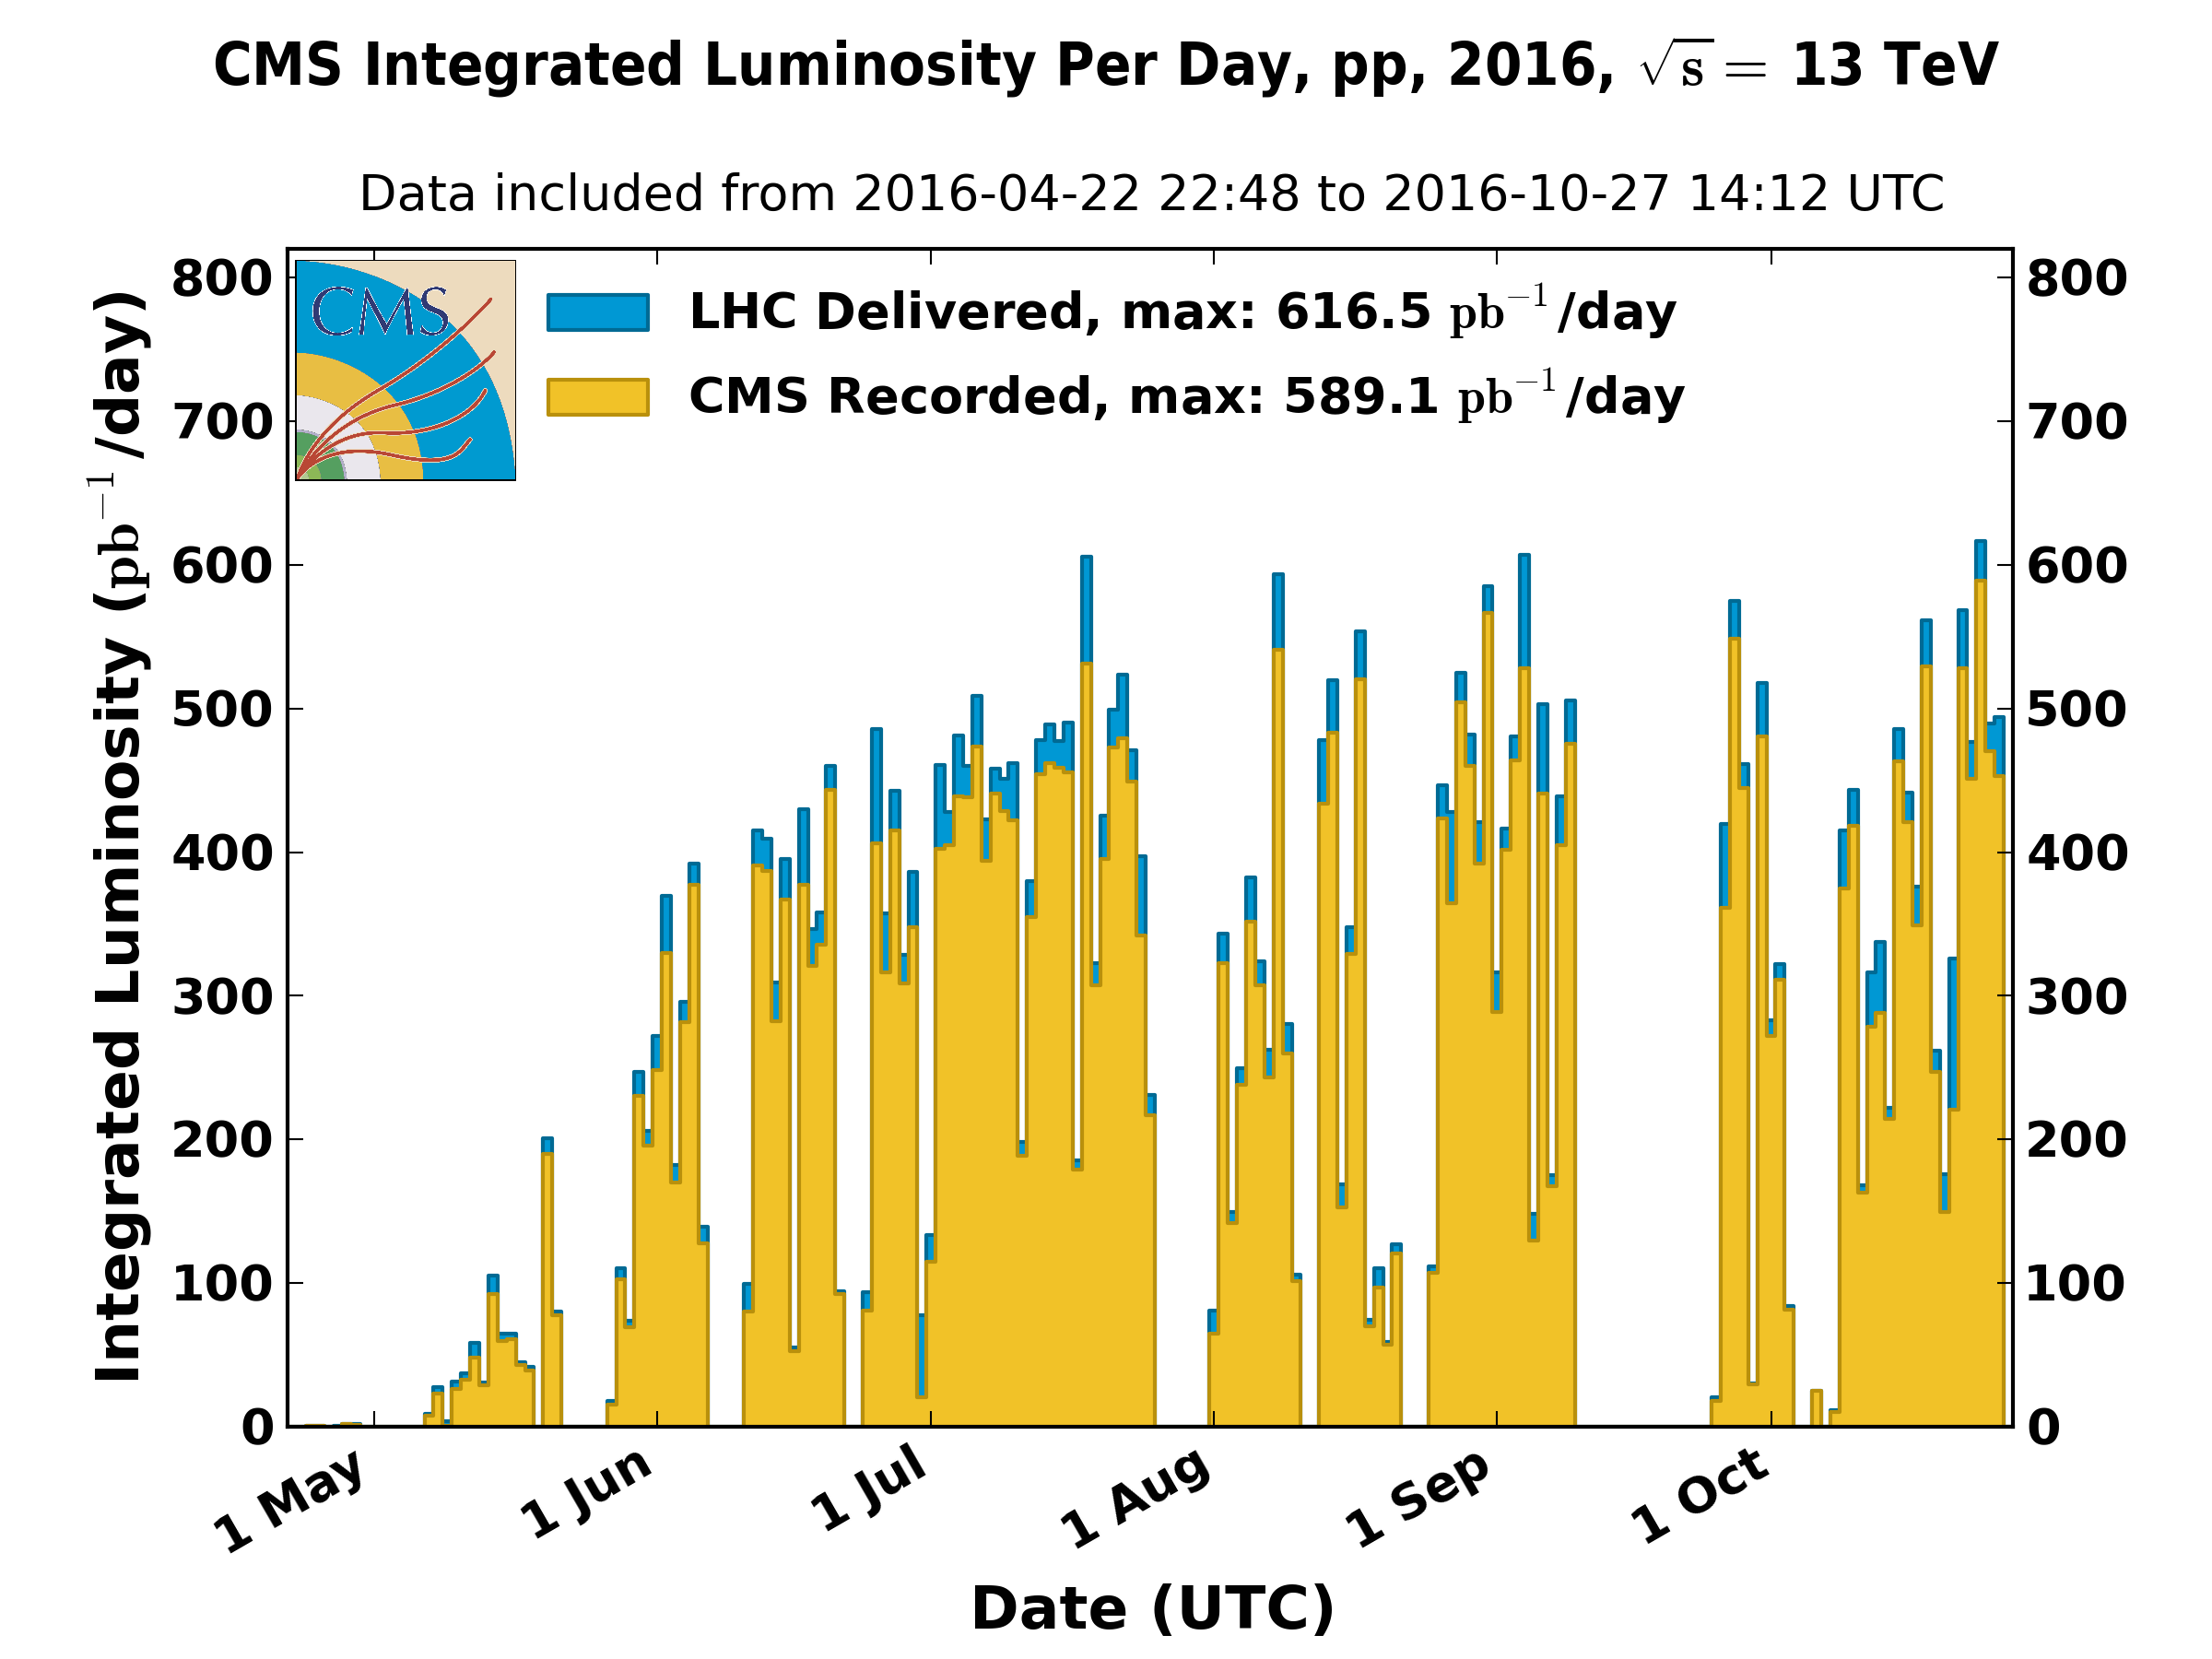
\includegraphics[scale=0.39]{fig/chapt3/int_lumi_per_day_pp_2016.png}
& \hspace{-0.5cm} 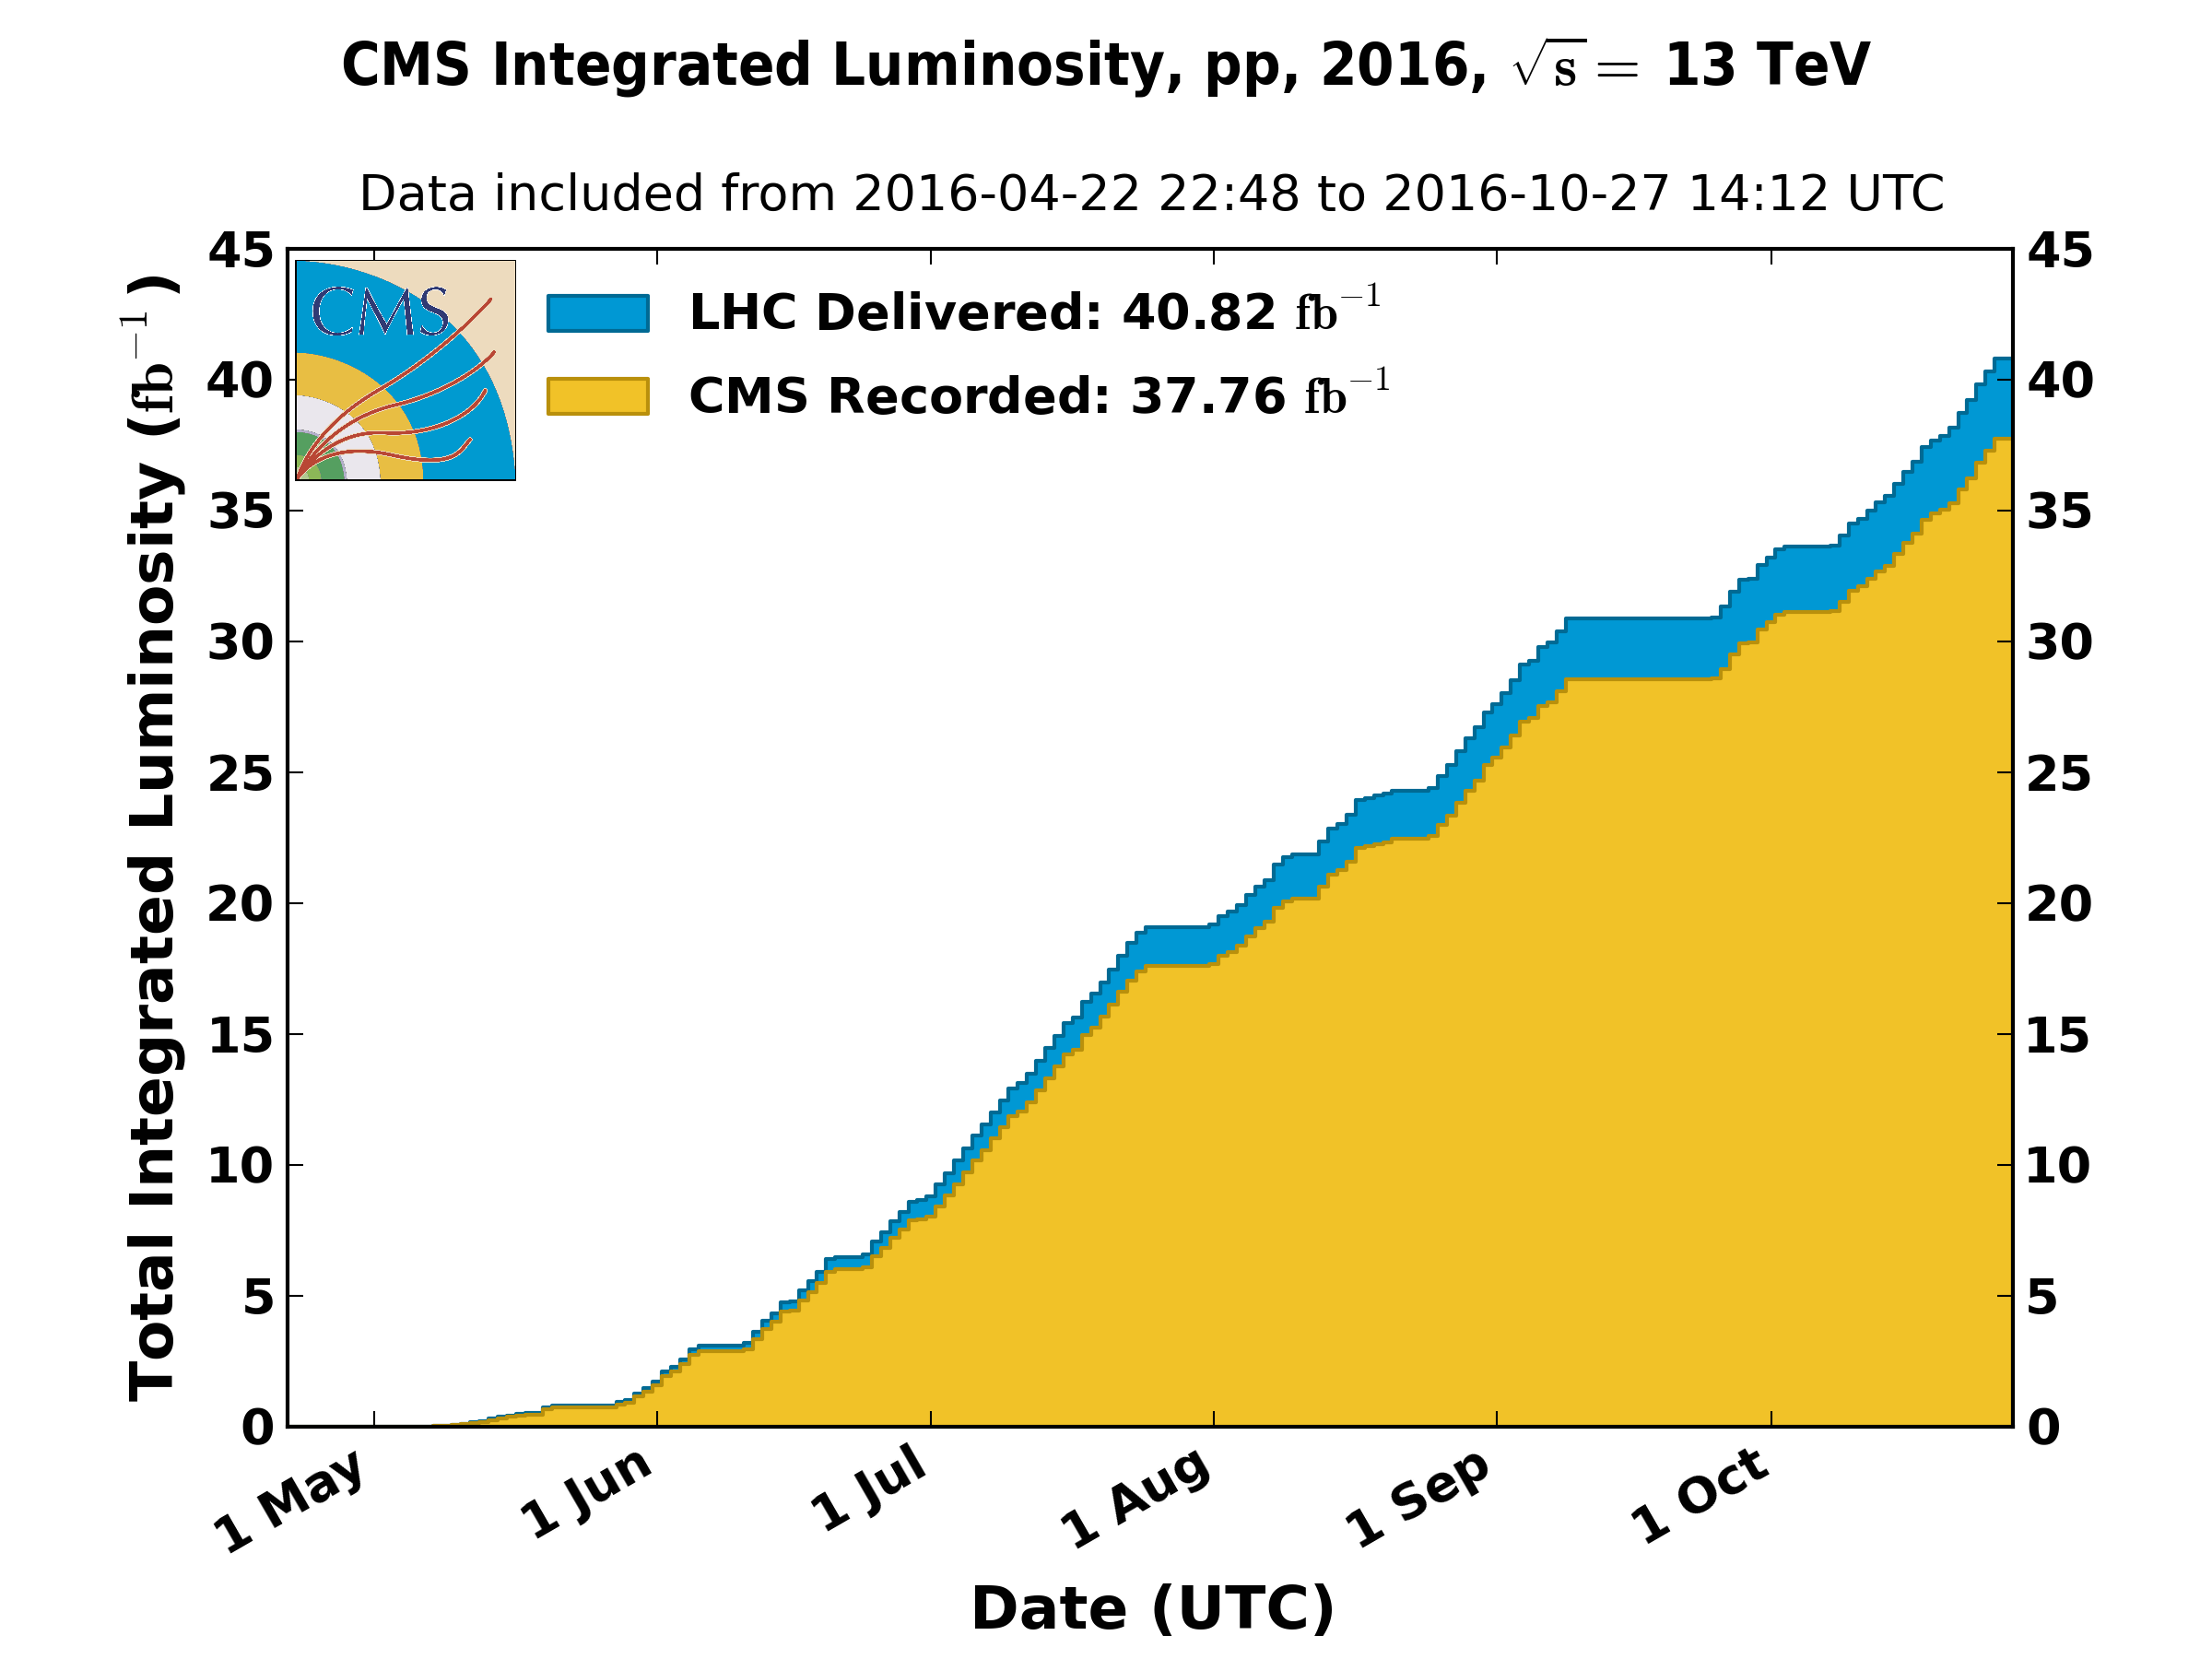
\includegraphics[scale=0.39]{fig/chapt3/int_lumi_per_day_cumulative_pp_2016.png}\\
   ($\mathbf{a}$)\qquad&($\mathbf{b}$)\qquad\\
\end{tabular}
\caption{The evolution of the instantaneous luminosity per day (a) and the integrated luminosity (b) delivered by the LHC (blue) and recorded by CMS (yellow) in 2016. The plots are taken from online cmstwiki \cite{twiki:cms_lumi}.}\label{fig:cms_lumi}
\end{figure}

Among the four detectors, two of them ATLAS (A Toroidal LHC ApparatuS) and CMS (Compact Muon Solenoid) are the largest and multi-purpose experiments. Their main focus is on the precise measurements of the SM as well as searches of BSM physics. ALICE (A Large Ion Collider
Experiment) is designed for heavy-ion collisions to study the physics of strongly interacting matter at extreme energy densities; and to study the quark-gluon plasma. Hadron Collider beauty (LHCb) experiment is designed to study the heavy flavour beauty hadron physics.

\section{The CMS Experiment at LHC}\label{sec:cms}
The CMS \cite{cms_exp} is one of the two multi-purpose experiments installed at the LHC cavern with a design to study a wide range particle and heavy ion physics measurements. Its primary goals are to elucidate the nature of the electroweak symmetry breaking mechanism linked to the Higgs mechanism, the search for physics Beyond the Standard Model (BSM) and the precise measurements of SM processes. An overview of the whole detector is shown in Fig. \ref{fig:CMS_exper}. The general concept driving the detector design is the configuration of the magnetic field needed to bend the trajectory of the charged particles, especially muons, to have good resolution in measuring high momentum. The CMS detector has a superconducting solenoid magnetic, producing a field of 3.8 T parallel to the beam axis, encapsulates a high-quality tracking system and calorimeters. The muon system is installed outside the magnet in 4 stations and interleaved with return yoke. The magnetic field is strong enough to saturate 1.5 m of iron. Each muon station consists of several layers of aluminium drift tubes (DT) in the barrel region (coaxial to the beam axis) and cathode strip chambers (CSCs) in the endcap region (perpendicular to the beam axis), complemented by resistive plate chambers (RPCs). The CMS detector is relatively compact in spite of its heavy weight, 12,500 Tons, (compare to ATLAS) with a length of 21.6 m and a diameter of 14.6 m. \\
\begin{figure}[h!]
%\centering
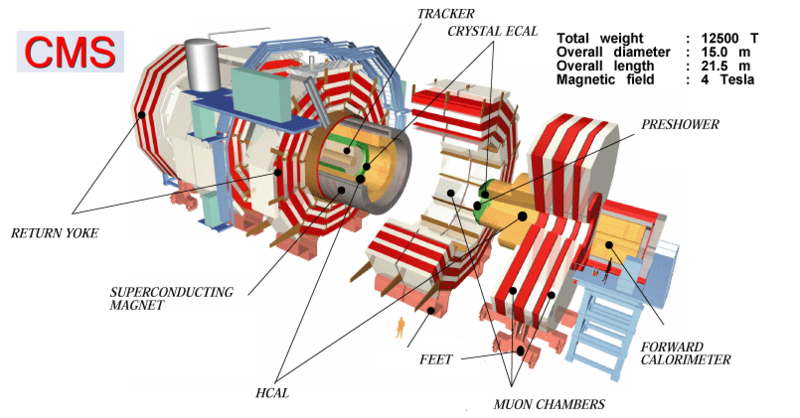
\includegraphics[width=1.05\textwidth]{fig/chapt3/CMS_exper.png}
%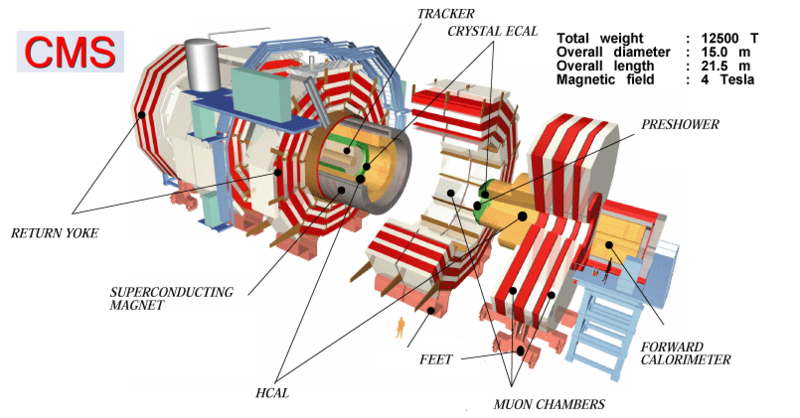
\includegraphics[scale=0.4, trim=20 50 60 30,clip]{fig/chapt3/CMS_exper.png}
\caption{\label{fig:CMS_exper} An overview of the CMS detector showing the major sub detectors.}
\end{figure}
The CMS experiment adopted a cylindrical coordinate system with its origin at the nominal interaction point in the center of the detector.    The direction of the z-axis is chosen along the anti-clockwise beam and it is referred as longitudinal. The x-axis points radially towards the center of the LHC ring and the y-axis is vertical and pointing upwards shown in Fig.\ref{fig:CMS_coordinates}. 
\begin{figure}[h!]
\centering
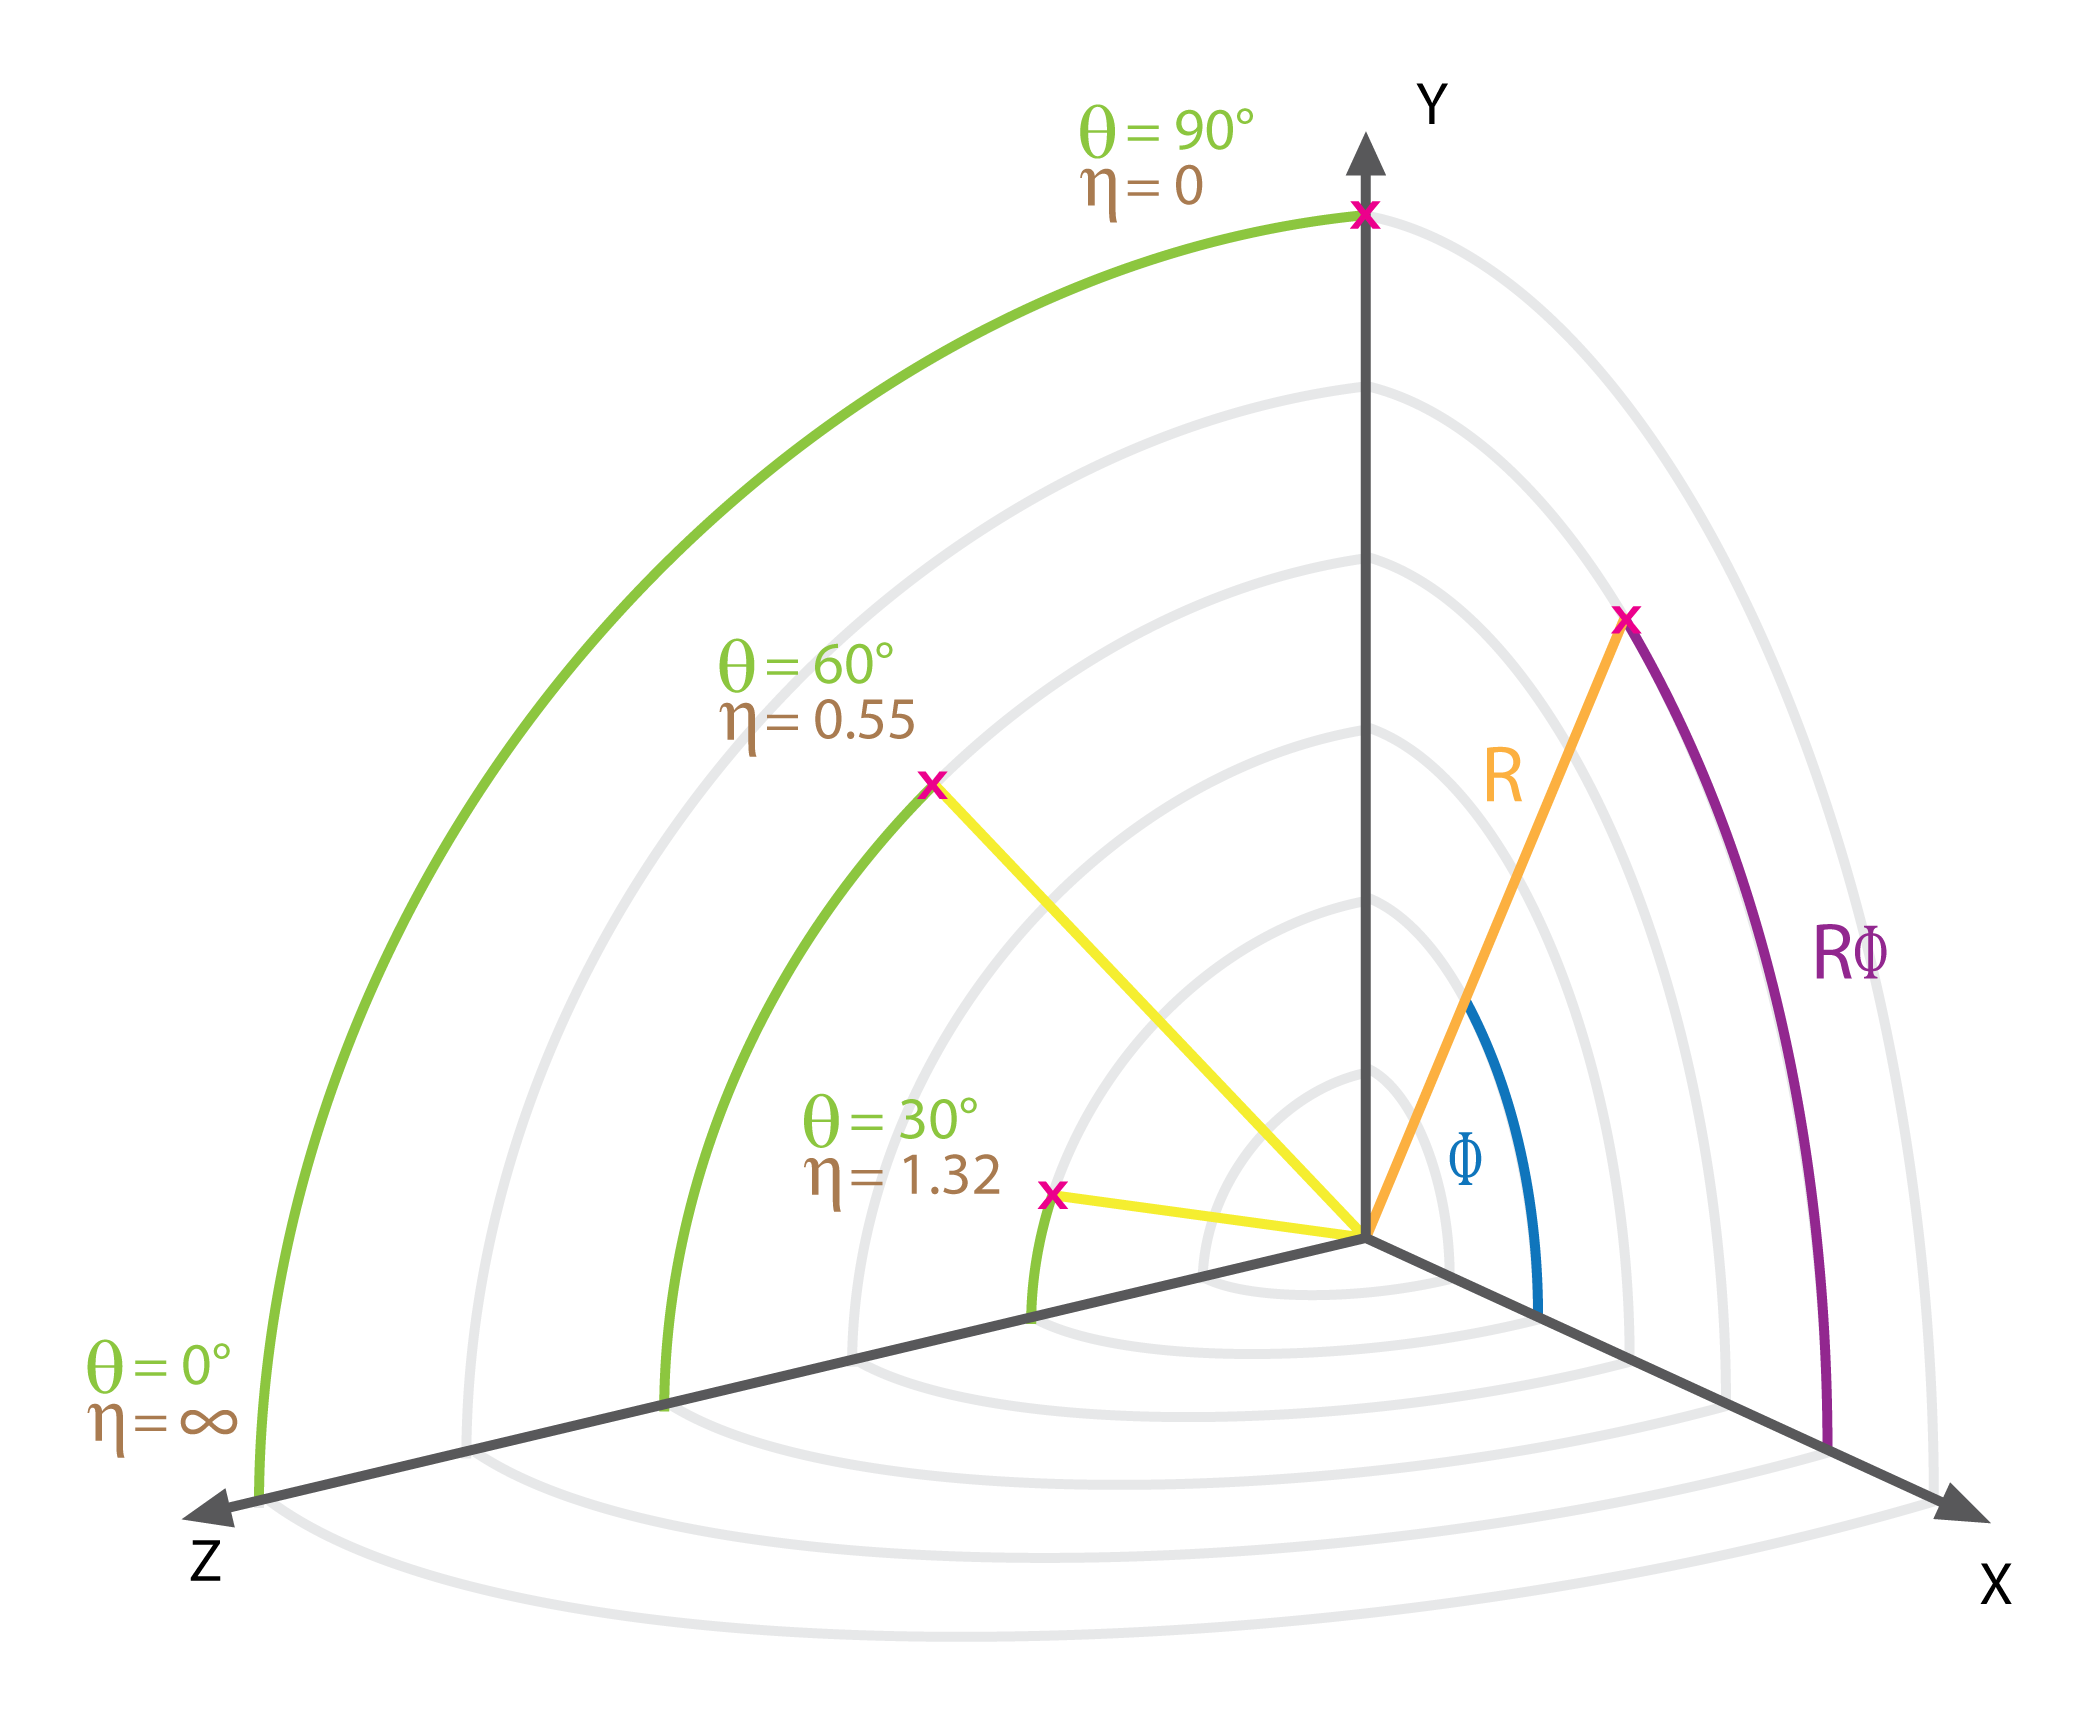
\includegraphics[width=0.6\textwidth]{fig/chapt3/img_cms_coordinates.png}
\caption{\label{fig:CMS_coordinates} An overview of the CMS experiment coordinate system.}
\end{figure}
The azimuthal angle $\phi$ is measured from x axis in the x-y plane where x-y plane is perpendicular to the beam axis and called transverse plane. The polar angle $\theta$ is measured from the z-axis. Instead of $\theta$, angular position is preferentially expressed in terms of a kinematic quantity called pseudorapidity ($\eta$), defined as:
\begin{equation}
\eta \equiv -ln(tan(\frac{\theta}{2}))
\end{equation}
Adopting the above coordinate system, a particle momentum $p$ has two components, one is transverse to the beam direction denoted by $p_{T}$ and calculated from x and y components. The second component is the longitudinal one, $p_{z}$, pointing along the z-axis. Missing transverse energy $E_{T}^{miss}$ term is used for imbalance in total transverse energy of a collision. The angular separation between two particles is usually expressed in $\phi-\eta$ plane expressed as:
\begin{equation}
\Delta R = \sqrt{\Delta\Phi^{2} + \Delta\eta^{2}}
\end{equation} 
In the following sections, a brief summary of all the subsystems of the CMS experiment is given.

%================================================
\subsection{Tracker}
The tracker is the innermost and closest to the interaction point, sub-detector of CMS, immersed in the homogeneous magnetic field of 3.8 T provided by the solenoid.  It is designed to measure the momentum and charge of charged particles emerging from the interaction point by determining the bending of their trajectories in their passage through the detector layers. Secondary vertices can also be reconstructed, associated to the late decays of particles such as B hadrons. The trajectory deviation from the straight line propagation is measured by the sagitta:
\begin{equation}
s \approx \frac{0.3BL^{2}}{8p_{T}}
\end{equation}
Where s is sagitta, B is the solenoid magnetic field, L is the track length and $p_{T}$ is the transverse momentum. The transverse momentum resolution is mainly dependent on the geometric accuracy on the sagitta ($\sigma_{s}$), through:
\begin{equation}
 \frac{\sigma_{p_{T}}}{p_{T}} \approx \frac{8p_{T}}{0.3BL^{2}}.\sigma_{s}
\end{equation}
At the LHC design luminosity and energy (around 1 MHz/mm$^{2}$ at 4 cm from the beamline), several hundreds of particles go through the tracker during each bunch crossing, high granularity, fast response and high radiation tolerance are especially important to its design. To fulfil the aforementioned criteria, the semiconductor silicon technology was chosen to build inner tracking system \cite{tracker}. Charged particles traversing a sensor produce electron-hole pairs which drift under an applied electric field, giving rise to a current pulse. Cooling is ensured by liquid perfluorohexane, maintaining the sensor temperature at around \SI{-10}{\celsius} to limit noise due to radiation-induced leakage\\ 
The tracker occupies a cylindrical volume of 5.8 m in length and 2.5 m in diameter with a surface area of 210 m$^{2}$, extends in the region of $\abs{\eta}$ < 2.5, r < 120 cm, $\abs{z}$ < 270 cm. A schematic view of the CMS tracker is shown in Fig.\ref{fig:tracker}. 

\begin{figure}[h!]
\centering
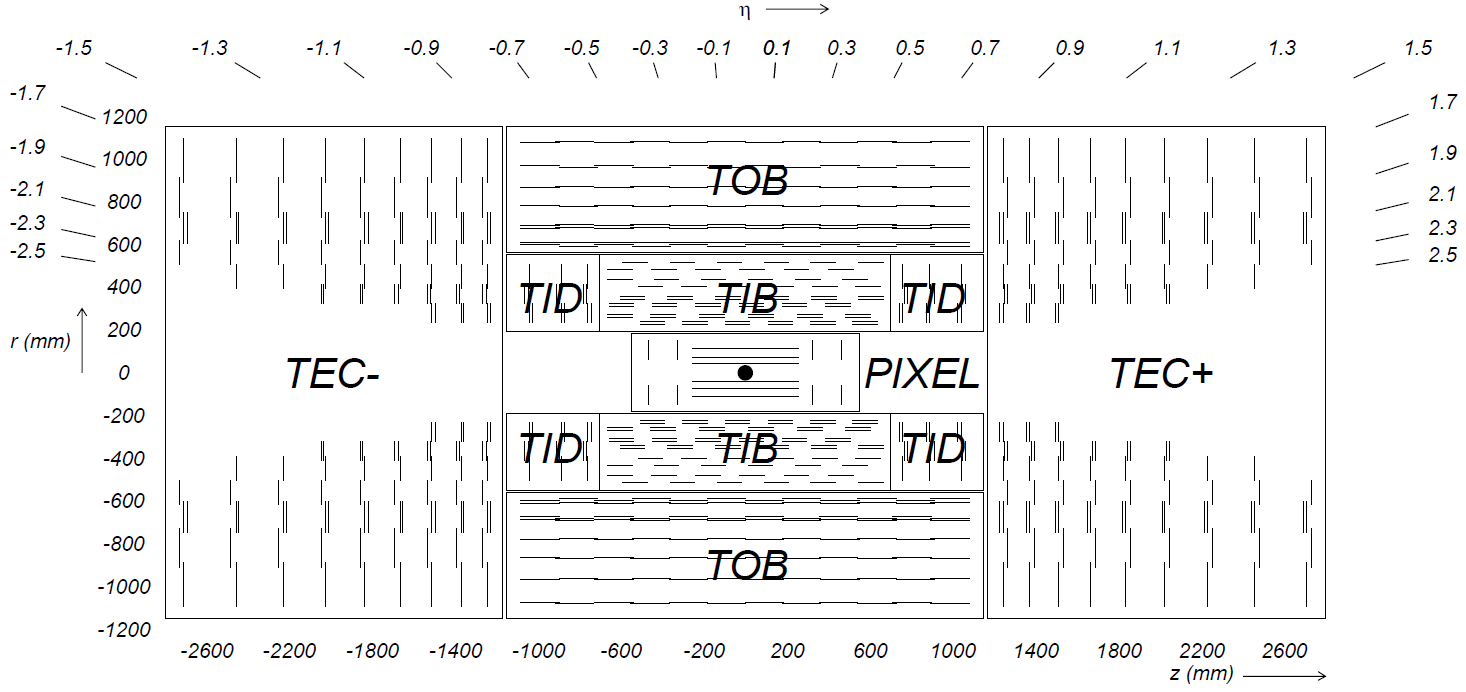
\includegraphics[scale=0.3]{fig/chapt3/Tracker.png}
\caption{\label{fig:tracker} The CMS tracker system with its subsystems in (r, z) plane.}
\end{figure}
The tracker has two sensors classes,  pixel and strip detectors.
\begin{itemize}
\item{\textbf{Pixel Tracker System:}} is placed closest to the interaction point (r $\leq$ 10cm), because of the largest track density. It comprised of a total of approximately 66 million pixel cells grouped in 1440 modules with a cell size of 100 $\times$ 150 $\mu$m$^{2}$. They are arranged in three cylindrical barrel layers at radii between 4.4cm and 10.2cm from the beam line and two endcap discs at each side of the barrel approximately 34.5cm and 46.5cm from the interaction point. With a high reconstruction hit efficiency well above 99\%, the pixel detector covers a pseudorapidity range $\abs{\eta}$ < 2.5, corresponding to the acceptance of the entire tracker. The typical spatial hit resolution is measured to be about 10$\mu$m in the $r-\phi$ plane and 15$\mu$m along the z-axis, while the third coordinate is given by the sensor plane position, allowing for a three-dimensional vertex reconstruction.
\item{\textbf{Strip Tracker System:}} occupies the outer part of the tracker cope with reduced particle density. The silicon strip detector is made of two concentric sets of layers in the barrel (TIB and TOB) occupying the region 20cm < $\abs{r}$ < 55cm and $\abs{z}$ < 118cm and two blocks of forward disks in the endcaps, called TEC and TID covering the region with 55cm < $\abs{r}$ < 116cm and $\abs{z}$ < 118cm.  The single-point resolution is of about 30$\mu$m in the $r-\phi$ plane and 300$\mu$m in the z direction.
\end{itemize} 

%================================================
\subsection{Electromagnetic Calorimeter (ECAL)}
The CMS Electromagnetic CALorimeter (ECAL) \cite{ecal} is an hermetic, homogeneous and high-granularity system made of inorganic scintillating crystals. It's primary aim is to measure precisely position and energy of electrons and photons, which induce electromagnetic showers in the material. The physics process that driven the design of the ECAL is the low mass Higgs decay into two photons $H \rightarrow \gamma\gamma$, one of the leading channels for the study of the Higgs properties. It's role in the $H \rightarrow ZZ \rightarrow 4l$ channel is also important in reconstructing electron together with tracker. ECAL technology is based on lead tungstate (PbWO$_{4}$) scintillating crystals, which act both as absorbers with a short radiation length (X$_{0}$ = 0.89cm) and as scintillators with a very fast response (80\% of the light is emitted within 25ns) which cope with the LHC bunch spacing. Avalanche photodiodes (APD) is used in the barrel and vacuum phototriodes (VPT) in the endcaps to detect the scintillation light with wavelengths around 420nm. An overview of the CMS ECAL is shown in Fig.\ref{fig:ecal}.
\begin{figure}[h]
\centering
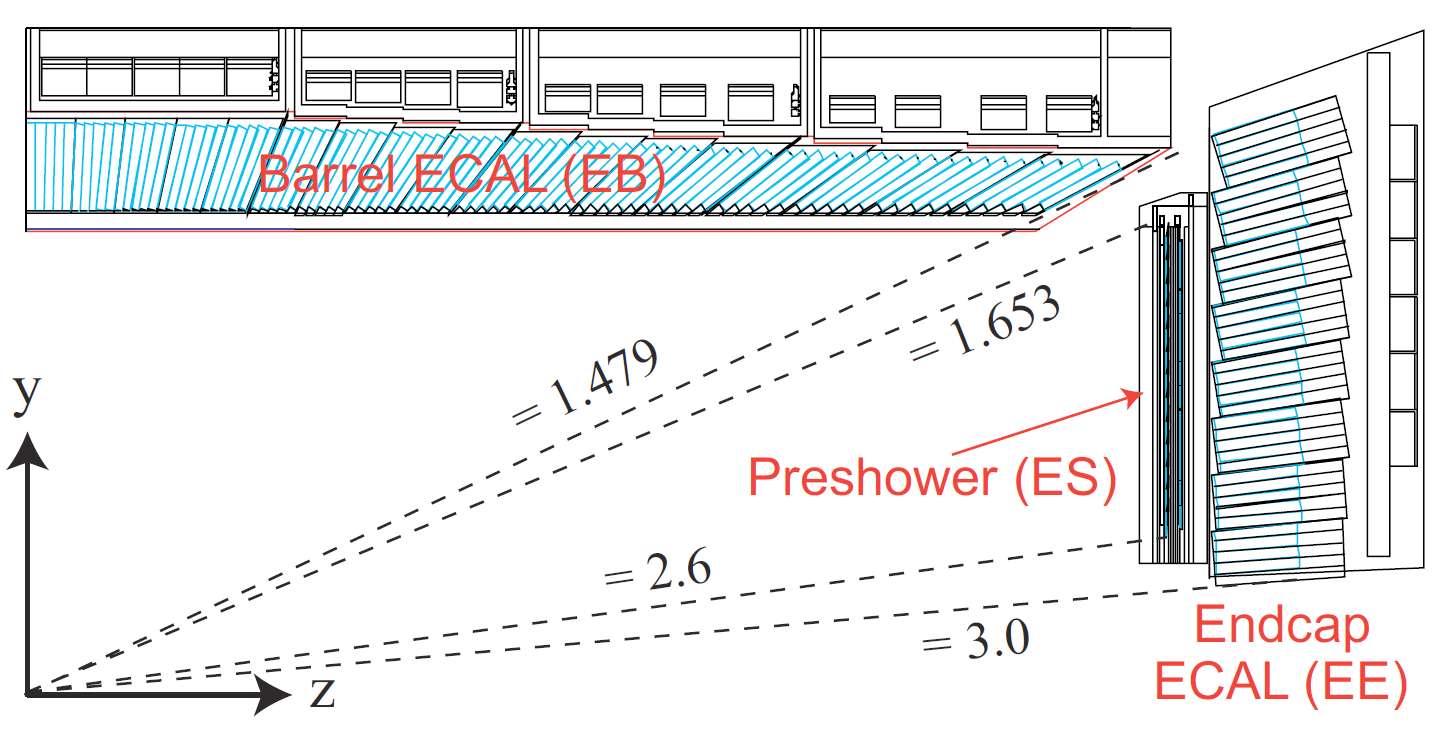
\includegraphics[scale=0.3]{fig/chapt3/img_ECALRapidity.png}
\caption{\label{fig:ecal} The ECAL longitudinal overview of a quadrant.}
\end{figure}
\begin{itemize}
\item{\textbf{ECAL Barrel (EB):}} is located at a distance r = 129cm from the beam axis and it covers the pseudorapidity range 0 < $\abs{\eta}$ < 1.48. It is equipped with 61,200 crystals with a high granularity of 0.0174 $\times$ 0.0174 rad in $\eta-\phi$, each with a transverse section of 22 $\times$ 22 mm$^{2}$ at the front face and a length of 230mm (25.8X$_{0}$). Crystals are grouped in arrays of 2 $\times$ 5, contained in a very thin 200$\mu$m alveolar structure, each corresponding to a sub-module. A group of 40/50 sub-modules are further assembled in modules, where four modules make a super-module.  Finally, EB is divided into 36 super-modules, each subtending an angle of \SI{20}{\celsius} in $\phi$. 
\item{\textbf{ECAL Endcaps (EE):}} is located at a distance $\abs{z}$ = 315.4cm from the interaction point and it covers the range 1.479 < $\abs{\eta}$ < 3 with identically shaped crystals, grouped in carbon-fiber structure of 5 $\times$ 5 elements, called super-crystals. The crystals have a rear face cross section of 30 $\times$ 30 mm$^{2}$, a front face cross section of 28.62 $\times$ 28.62 mm$^{2}$ and a length 220mm (24.7X$_{0}$). Each EE has 134 identical supercrystals with a further 18 sectioned supercrystals to complete the inner and outer perimeter.
\item{\textbf{ECAL Preshawer (ES):}} detectors are placed at each end of the tracker, in front of the EE and cover the pseudorapidity range 1.653 < $\abs{\eta}$ < 2.6. It is a two-layer sampling calorimeter consisting of lead radiator layer with a total of 3X$_{0}$ that initiates electromagnetic showers from incoming particles, and silicon strip sensors that measure the deposited energy and transverse shower profiles. The ES help distinguish $H \rightarrow \gamma\gamma$ decays from single photons, and to identify electrons against minimum ionizing particles.
\end{itemize}
The ECAL energy resolution $\sigma$(E) (for energies below 500 GeV) is given as:
\begin{equation}
(\frac{\sigma_{E}}{E})^{2} = (\frac{S}{\sqrt{E}})^{2} + (\frac{N}{E})^{2} + C^{2}
\end{equation}
where S is the stochastic term due to fluctuations in the lateral shower containment, photostatistics and preshower energy deposition, the second term quantifies the effect of electronic noise and pileup and the constant term is related to the non-uniformity of the longitudinal light collection, calibration uncertainties and energy leakage from the back. The performance of the ECAL barrel module has been studied based on measurements with test-beam data, the typical values of these three parameters obtained are S = 2.8\%, N = 12\% and C = 0.30\% \cite{ecal_resol};

\subsection{Hadronic Calorimeter}
The CMS hadronic calorimeter (HCAL) \cite{hcal} is a hermetic sampling calorimeter, measures precisely the energy and position of charged and neutral hadrons in the form of jets. It also provides an indirect measurement to non-interacting particles in terms of missing energy ($E_{T}^{miss}$). HCAL surrounds the ECAL and the design is restricted by the geometrical dimensions of the ECAL
and magnet systems. A schematic overview of the HCAL is shown in Fig.\ref{fig:hcal} with its four sub-detectors.
\begin{figure}[h!]
\centering
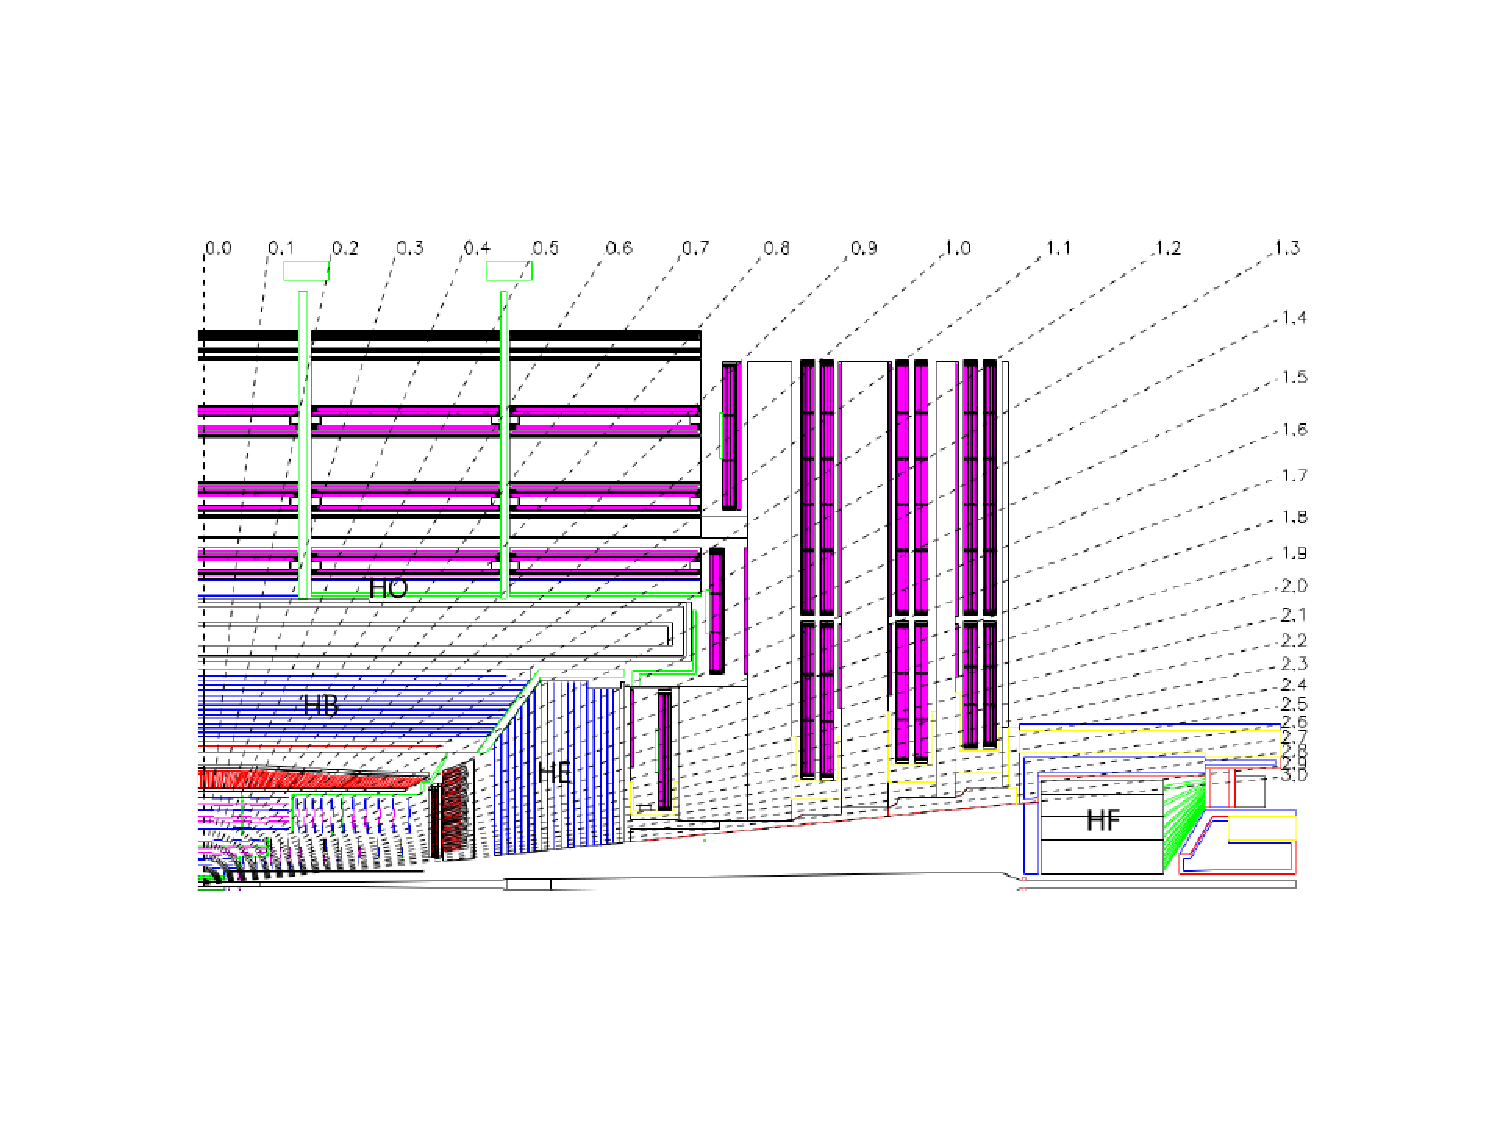
\includegraphics[scale=0.8, trim=90 100 80 80,clip]{fig/chapt3/HCAL.pdf}
\caption{\label{fig:hcal} Longitudinal overview of the one quadrant of the CMS HCAL.}
\end{figure}
The HCAL Barrel (HB) comprise of two half-barrel sections covering a total pseudorapidity range of $\abs{\eta}$ < 1.3, located between EB with r = 1.77m and the inner extent of the magnet coil (r = 2.95m), corresponds to interaction lengths of 5.82$\Lambda_{I}$ in the central region. Due to space restriction, the HB is complemented by an additional layer of scintillators outside the solenoid, referred to as the hadronic outer (HO) calorimeter. HO provides additional depth up to a minimum 11.8$\Lambda_{I}$ to the HCAL system in the radial direction and have same characteristics as HB. \\
The HCAL Endcap (HE) covers forward region in pseudorapidity range of 1.3 < $\abs{\eta}$ < 3.0 and has sufficient depth around 10$\Lambda_{I}$. HB and HE use non-magnetic brass layers as absorber material, and are interspersed with plastic scintillator tiles which serve as the active medium. Two forward hadron calorimeters (HF) are installed which cover the very forward region in pseudorapidity given by 3.0 < $\abs{\eta}$ < 5.0, positioned at $\abs{z}$ = 11.2m from the interaction point, thus ensuring good hermeticity. HF detectors using steel as absorber and Cherenkov-light-emitting quartz fibres are as active medium, motivated by the high particle flux in this region.  The energy resolution of the HCAL system can be expressed in stochastic term a and constant term b as:
\begin{equation}
(\frac{\sigma_{E}}{E})^{2} = (\frac{a}{\sqrt{E}})^{2} + b^{2}
\end{equation}
%=========================================================
\subsection{Magnet}
The CMS detector uses solenoid magnetic field which is the core part of the detector and giving name to the detector. A strong magnetic field is needed to achieve good resolution of the high momentum charged particle upto 1TeV by measuring curvature while direction gives charge of particle \cite{cms_magnet}. The structure of superconducting magnet for CMS  has 6m diameter and 12.5m length, able to generate a uniform magnetic field of 3.8T with a stored energy of 2.3 GJ at full current of 19500A. A graphical overview of the CMS magnetic field is shown in Fig.\ref{fig:magnet}. The magnet mainly uses a superconducting coil (ensured by a helium cooling system at temperature 4K), a vacuum tank (responsible to isolate it from the external environment) and the 10000 ton magnet yoke comprising 5 wheels and 2 endcaps (necessary to return magnetic flux, which otherwise would get lost, disturbing the surrounding environment). 
\begin{figure}[h]
\centering
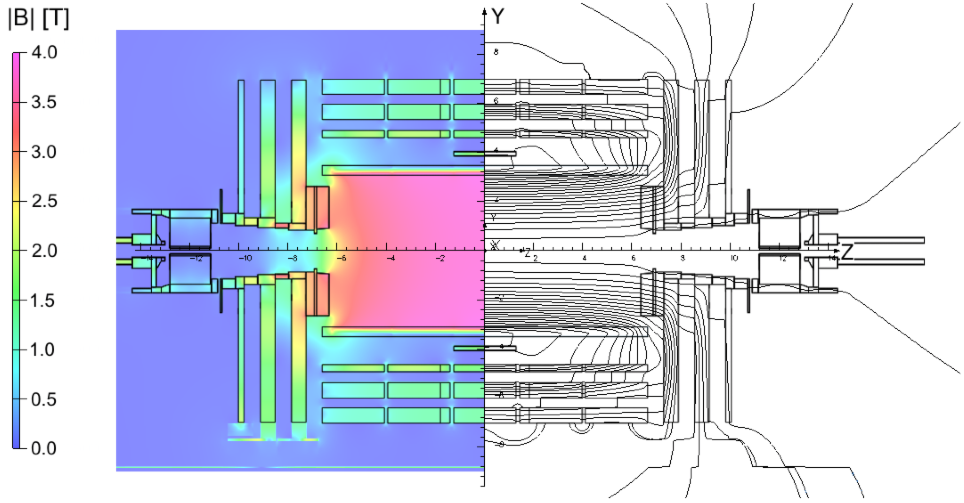
\includegraphics[scale=0.4]{fig/chapt3/Sections_IntroductionFigs_MagField.png}
\caption{\label{fig:magnet} Longitudinal view of the CMS detector magnet where left side shows simulation of the magnetic field and the magnetic field lines are at the right side. At the heart of the detector, the magnetic field value is 3.8T.}
\end{figure}
%========================================
\subsection{Muon Spectrometer}
Muon plays a key role in search for many physics phenomena, ranging from precise measurement of the SM of particle physics to new searches, especially in the discovery of the SM higgs boson through golden channel ($H\rightarrow ZZ \rightarrow 4l$). Being a massive particle compared to electron, muon is less effected by Bremsstrahlung radiations and travel through all the detector subsystems. Using this characteristics, the muon system in the outer region of the CMS detector is embedded in the return yoke of the solenoid. Muons bring a very clean signature to its spectrometer because other particles are stopped by the calorimeters. The CMS muon spectrometer covers a pseudorapidity range to $\abs{\eta}$ < 2.4, consists of three subsystems, Drift Tubes (DTs), Cathode Strips Chambers (CSCs) and Resistive Plate Chambers (RPCs) \cite{cms_muon} as shown in Fig.\ref{fig:rpc_dt}.   

\begin{itemize}
\item{\textbf{Drift Tubes:}}
In the barrel region of the CMS muon system where the magnetic field is mostly uniform and the muon rate is low, four layers of muon stations are installed consists of drift tube (DTs) chambers, covers the pseudorapidity region $\abs{\eta}$ < 1.2. In each wheel, DTs are installed into 12 $\phi$-segments, forming 4 stations in radial direction and interleaved between plates of the magnet flux return yoke. In the longitudinal (except MB4) and bending plane, each station consists of 4 and 8 layers of DTs respectively, to measure precisely the position.\\
DTs consists of an individual cell with grounded walls, acting as cathode and a 50$\mu$m diameter gold-plated stainless-steel anode wire at the center of the cell. The drift electric field is created by two electrode plates mounted at the two sides of the cell. The cells use a gas mixture of 85\% of Ar and 15\% CO$_{2}$ with HV settings: V$_{wire}$ = +3600V, V$_{cath}$ = -1800V and V$_{strip}$ = +1800V \cite{muon-sys}.  
\item{\textbf{Cathode Strip Chambers:}}
Cathode Strip Chambers (CSCs) are installed in the endcap regions with pseudorapidity coverage 0.9 < $\abs{\eta}$ < 2.4. The muon rate and background radiations are higher at the endcaps combine with non-uniform magnetic field, motivated the CSCs to have a fast time response, radiation tolerance and finely segmented. The CSCs operate as standard multi-wire proportional counters, comprise of six planes of anode wires interleaved among seven cathode strips. The anode wires run azimuthally and identify the radial component of a track hit. The cathode strips are oriented radially, almost perpendicular to the wires and provide a precision measurement in the r-$\phi$ bending plane. The CSCs system uses a nominal gas mixture of 40\% Ar, 50\% CO$_{2}$ and 10\% CF$_{4}$.

\item{\textbf{Resistive Plate Chambers:}}
The CMS muon system comprises of a third type of muon detectors, Resistive Plate Chambers (RPCs), installed both in the barrel and endcap regions along with DTs and CSCs, covers the full pseudorapidity range $\abs{\eta}$ < 1.6. RPCs are gaseous parallel-plate detectors, operating in avalanche mode and capable of tagging the time of an ionizing event in times less than 25ns (the bunch crossing time at the design luminosity of the LHC). It makes RPCs an ideal trigger system that provides correct bunch crossing time information between two successive bunches with muons, even at the largest LHC luminosities.
The basic module of the CMS RPC consists of a double-gap chamber where each gap separates two parallel plates of bakelite with a bulk resistivity of 10$^{10}$ - 10$^{11}\Omega$cm. A gas mixture of 95.2\% C$_{2}$H$_{2}$F$_{4}$, 4.5\% i-C$_{4}$H$_{10}$ and 0.3\% HF$_{6}$ using in RPC operation where C$_{2}$H$_{2}$F$_{4}$ is ionized by incident particles and the other two gases prevents the detector from streamer mode. The RPCs operational voltage is lower than 10kV with efficiency about 100\%. Two gases used in RPCs named C$_{2}$H$_{2}$F$_{4}$ and HF$_{6}$ are not environmental friendly that should be replaced by other gases. To cover the full pseudorapidity $\abs{\eta}$ < 2.4 in the endcap region, the present design of the RPC is not suitable to face high flux of particles at the design luminosity of the LHC. A dedicated study is ongoing in the GIF++ facility which summarized in chapter \ref{chapt:10}  
\end{itemize}
\begin{figure}[h]
\centering
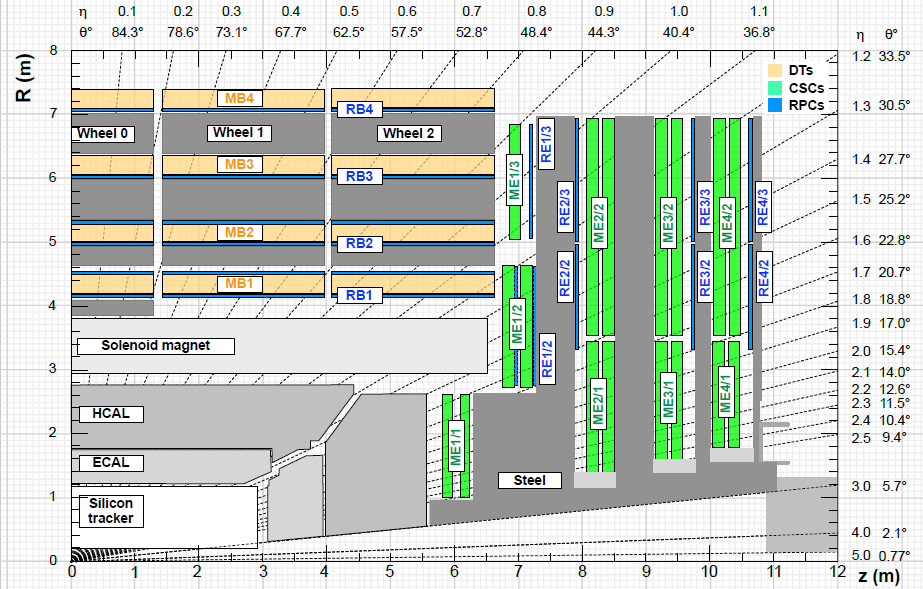
\includegraphics[scale=0.63]{fig/chapt3/muon_detectors.png}
\caption{\label{fig:rpc_dt} The CMS muon system in (R,z) cross section in a quadrant. z is coaxial with beam axis while R is perpendicular pointing upward. DTs are shown by light orange, CSTs by green and RPCs by blue color.}
\end{figure}

%==============================
\subsection{Trigger and Data Acquisition Systems}
The design bunch crossing time of the LHC is 25ns that corresponds to 40MHz frequency and have an average of 20 p-p collision per bunch crossing. This produces an enormous amount of data with 1MB size per event. Due to limitations of detector performance and storage system, the event rate needs a filter to suppress the rate to few hundreds of events per second. CMS uses a dedicated two level (level-1 and level-1) trigger system to control the event rate \cite{cms_trigger}.\\
\textbf{L1 Trigger}: the hardware based trigger system that reduces the rate to 100kHz with a maximum decision time of 4$\mu$s per event. Because of the short decision time, it only uses the calorimeter and muon system information with no tracker information. Local triggers reconstruct primitives particles candidates in each component of a given subdetector which are combined by regional triggers to construct higher level L1 objects (muons, electrons and jets) and subsequently merged into global trigger which decides to select or reject the event. \\
\textbf{HLT}: After the L1 trigger, event rate is further reduced to 40Hz by using high level trigger (HLT), a software based trigger that uses information from all subsystems. The reconstruction and selection used by HLT software is similar to the offline reconstruction and selection which takes place in two successive stages follow the basic principle of time minimization for each event. In first stage (Level-2), HLT takes input from L1 and reconstructs the basic objects from calorimeters and muon system. In second step (Level-3) of the HLT, the full information from the tracker is accessed for track reconstruction and vertices. The event is finally selected and permanently stored for offline analysis if the requirements of at least one HLT path are met.

  



\clearpage{\pagestyle{empty}\cleardoublepage}

\graphicspath{{chapt_dutch/}{intro/}{chapt2/}{chapt3/}{chapt4/}{chapt5/}{chapt6/}{chapt7/}{chapt8/}}

% Header
\renewcommand\evenpagerightmark{{\scshape\small Chapter 4}}
\renewcommand\oddpageleftmark{{\scshape\small Signal Generation and Simulation}}

\renewcommand{\bibname}{References}

\hyphenation{}

\chapter[Signal Generation and Simulation]%
{Signal Generation and Simulation}\label{chapt:4}
\section{Monte Carlo simulation}\label{sec:mc_sim}
In high energy physics experiments, event modelling plays an important role to understand the collected data. A precisely modelled event maximizes the chance to find out new physics and make precision measurement of the Standard Model processes. However, in hadron-hadron colliders where the colliding particles are composite objects, like proton-proton in LHC, the event modelling is a challenging task. The same applies to particles interactions within the bulk of detector volume. These tasks can be solved by employing Monte Carlo generation techniques, incorporating the Standard Model, models of new physics and the detector effects while detecting final state particles in the interaction. An event occurs when two protons collide and produces a cascade of new particles as shown in figure \ref{fig:event}. Because of complexity of the event, the MC generators model the events in a simulation chain: hard interaction, parton showering, hadronization and decays. These processes are explained in the following sections.
\begin{figure}[h]
\centering
%\captionsetup{width=0.8\linewidth}
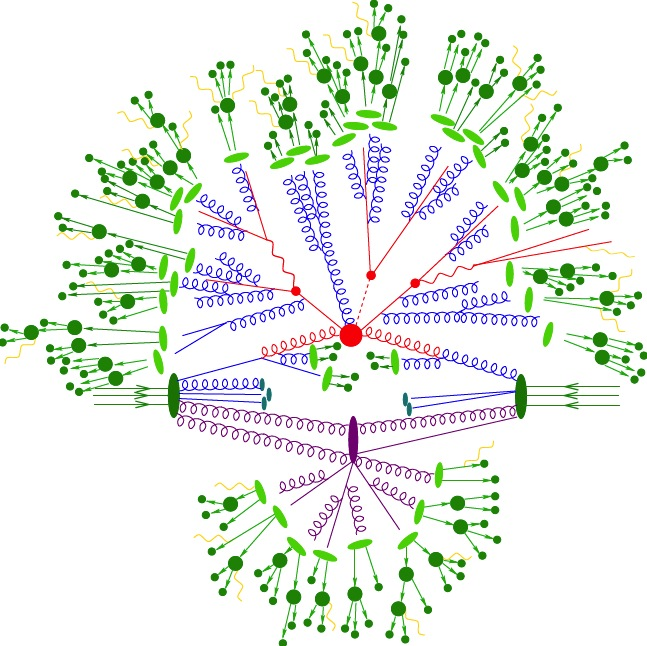
\includegraphics[width=0.6\textwidth]{fig/chapt4/event_sim.jpeg}
%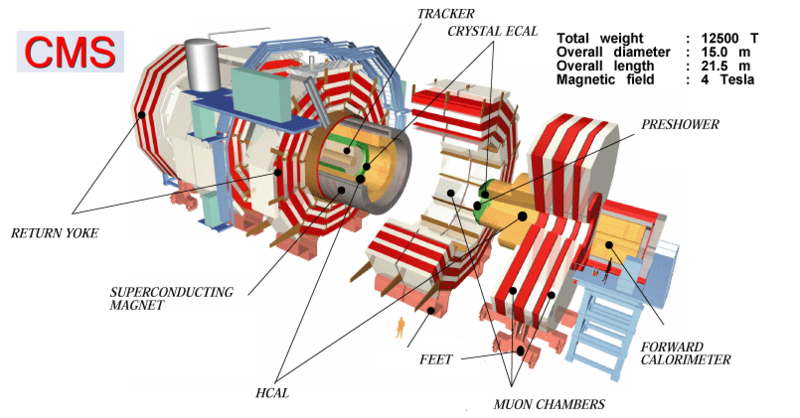
\includegraphics[scale=0.4, trim=20 50 60 30,clip]{fig/chapt3/CMS_exper.png}
\caption{\label{fig:event}Pictorial representation of a $pp$ collision event \cite{simulated_event}. The hard interaction shown by the big red blob. Additional hard QCD radiation is produced (red) and a secondary interaction takes place (purple blob) before the final-state partons hadronise (light green blobs) and hadrons decay (dark green blobs). Photon radiation occurs at any stage (yellow)}
\end{figure}  
\begin{itemize}
\item{\textbf{Hard scattering:}}
The actual interaction of two protons occurs when partons (constituents of proton - gluons or quarks -) from the two colliding protons interact and produce new particles with high $p_{T}$. These events are of keen interest for analysis and referred as hard scattering. If the colliding protons merely undergo soft collision, resultant particles have low $p_{T}s$, commonly known as soft scattering. The parton distribution functions (PDFs) describing the structure of the proton and contained the initial momentum distribution of the partons involved in the hard interaction. In hadron-hadron (in case of LHC it is $pp$) collisions, a wide variety of hard scattering cross sections can be calculated using the QCD factorization theorem and weighting the subprocess cross section with the PDFs extracted from deep inelastic scattering \cite{hard_scatter}. Factorization theorems separate long- and short-distance physics when calculating these cross sections.   
\begin{equation}\label{eq:xsec}
\sigma_{AB} = \int dx_{a}dx_{b}f_{a/A}(x_{a},\alpha_{s},\mu_{F}).f_{b/B}(x_{b},\alpha_{s},\mu_{F}).\hat{\sigma}(\hat{s};\alpha_{s},\mu_{F},\mu_{R})
\end{equation}  
where $f_{a/A}$ is the the probability that a parton $a$ inside a hadron $A$ carries a momentum fraction $x_{a}$, $\hat{s}$ is the parton center-of-mass energy, $\alpha_{s}$ is the strong coupling constant, $\mu_{F}$ is the factorization and $\mu_{R}$ is the renormalization scale.
\item{\textbf{Parton showering:}}
The previous section illustrates generation of a hard process according to lowest-order matrix elements that results in a limited number of partons in the final state. These describe the momenta of the outgoing jets well, but any fixed order is insufficient to give a complete picture of overall process including the internal structure of the jets and the distributions of accompanying particles. The effect of all higher-order corrections including additional ISR/FSR from the branching of the partons can be simulated through the parton-shower (PS) algorithm. It describes the evolution in momentum transfer down from the high energy scales associated with the hard process to the low scales, of order 1 GeV, associated with confinement of the partons it describes into hadrons \cite{parton_shower}. The multi-purpose event generators like PYTHIA \ref{subsec:pythia} and HERWIG \ref{subsec:herwig} used parton showering algorithms with different implementations. Hard processes can be described well using matrix element calculations where the partons are energetic and widely separated. It also incorporates the interference effects of amplitudes with the same final state topology. In this work we produce the interference effect between the signal ($gg\rightarrow H/A\rightarrow t\bar{t}$) and SM $t\bar{t}$ ($gg\rightarrow t\bar{t}$) background. Matrix element and parton shower algorithms can be combined to fully describe an event with an extra care to avoid double counting in the overlapping phase-space. Different schemes are using for this purpose. CMS uses MLM algorithm for matching to interface MADGRAPH with PYTHIA, which vetoes the emission of partons via showering above a user-defined matching threshold \cite{matching}.  
\item{\textbf{Hadronization:}}
Hadronization process starts after showering by which a set of colored partons is transformed into a set of color-singlet
primary hadrons, may decay further to secondary hadrons. Different models are in use to describe the fragmentation of the
partons after showering. The most commonly used one is the $Lund$ $String$ $Fragmentation$ $Model$, implemented in PYTHIA and proposed to be universal i-e process independent. It is based on the observation that the colour potential of the sources, such as a heavy quark–antiquark pair, increases linearly with their separation like a stretched string has $V(r) = \kappa r$. The potential energy increases with the separation of quark anti-quark and at order of 1 fm, it collapses into colour-field strings between them. The original quark pair are now converted into two pairs of quark and anti-quark $q\bar{q}\rightarrow q\bar{q}^{'} + q^{'}\bar{q}$ while this process continues until only hadrons remain \cite{hadronization}. Apart from the hard interaction, other constituents of the colliding proton can also interact, add additional hadrons in the final state. This is usually referred as underlying event (UE) described by special tunes in the generators like PYTHIA uses $CUETP8M2T4$ in this analysis. During one bunch crossing the average pp interaction goes up to 35, known as pileup, resulting into relatively low $p_{T}$ particles, but they can obscure the interesting hard process.
\end{itemize}
\section{Particle Physics Generators}\label{sec:gnerators}
In current High Energy Physics (HEP) regime, the most challenging part is the multiparticle production where the observed particles multiplicities extend to hundred. These multiplicities are expected to go upward in the future HEP colliders. Event Generators (EG), based on computer programs, solve this problem by generating events as detailed as could be observed by a perfect detector.   
In High Energy Physics (HEP), a number of Monte Carlo (MC) generators are available that calculate the tree-level diagrams numerically, and integrate over the relevant phase space. A list of them are used in monte carlo production for this analysis is discussed below.
\subsection{MadGraph}
MadGraph, now merged into MG\_aMC@NLO, a general-purpose event generator \cite{madgraph}, used for generation of the signal samples in this analysis. It is a pure matrix element generator that generates hadron-hadron ($pp, p\bar{p}, gg, q\bar{q}$) collision and in practice produces 8 particles (quarks, gluons and leptons) in the final state without hadronization. It also provides an opportunity to produce samples using interference effect. The interference comes into play when the signal and background have the same final state particles like in this analysis the signal is $gg\rightarrow H/A \rightarrow t\bar{t}$ and the standard model $t\bar{t}$, the main background, have same final state particles. 
MadGraph is further interfaced with Pythia or Herwig to generate showering and hadroziation steps. The double counting in the showering is solved by applying the MLM scheme. To describe the parton structure, NNPDF30 PDF \cite{pdf_sets} sets used in this analysis. 

\subsection{Pythia}\label{subsec:pythia}
Pythia is a multipurpose event generator used frequently in HEP. It provides the possibility to generate complete events, in as much detail as experimentally observable ones, within the bounds of our current understanding of the underlying physics. Pythia is used to model $e^{+}e^{-}$, $ep$ and $pp$ collisions and simulates a large variety (over 300) of hard 2 $\rightarrow$ 2 processes which include Standard Model and many beyond Standard Model processes upto Leading Order (LO) accuracy. Pythia uses Lund string model \cite{lund_string_model} to describe hadronization and external PDFs for hard processes calculations. It uses $p_{T}$-ordered showering technique for parton showering where partons are ordered by their transverse momentum ($p_{T}$) and $Q^{2} = p^{2}_{T}$ - the closer the parton approaches the vicinity of the hard process, the higher pT is assigned to it. A more detail about the Pythia program is given in \cite{pythia}.
\subsection{Powheg}
The Powheg (PositiveWeight Hardest Emission Generator) event generator \cite{powheg} provides the modeling of the hard interaction and needs to be interfaced with Pythia or Herwig for the parton showering and hadronization. Powheg models the hard process at NLO QCD accuracy. The proton structure is described by the PDF sets NNLOPDF30.
\subsection{MC@NLO}
The MC@NLO \cite{mcanlo} is an event generator which generates hard emission using NLO and MC approaches. For showering and hadronization, the MC@NLO has to be interfaced with general purpose detector like pythia. It also generates a small fraction of events with negative weights but in practice it is quite small. The PDF sets used by MC@NLO are NNPDF30.
\subsection{HERWIG}\label{subsec:herwig}
HERWIG is a general-purpose event generator \cite{herwig} which models hadron-hadron, lepton-lepton and hadron-lepton collisions at LO. Like Pythia, it provides the description of all subprocesses of an event but uses different approaches and algorithms. HERWIG tool implements an angular order showering, $Q^{2} \sim 1 - cos\theta$, where $\theta$ is the angle between parent and emitted parton. HERWIG exploits cluster model for showering.
\subsection{2HDMC and SusHi}\label{subsec:sushi}
\textbf{2HDMC:} Two-Higgs-Doublet Model Calculator \cite{2hdmc} is a general purpose calculator based on C++ code which can be used to study the phenomenology of a general ($\textsl{CP}$-conserving) two-higgs doublet model (2HDM) \ref{subsec:2hdm}. 2HDMC provided a user friendly interface to implement its favourite parameters space for the higgs potential. A user has fully control over the Yukawa sector by changing the coupling. The higgs masses, type of the model (type I and type II), alignment limit condition $sine (\alpha - \beta)$, the ratio of the vacuum expectation values of the doublet in 2HDM ($tan\beta$) and the scalar mass matrix, m$^{2}_{12}$, etcetera, can be specified with full freedom. The output of the 2HDMC consists of a check on the theoretical properties of the model like, $\textsl{CP}$-conservation, positivity and stability of the potential and the tree level unitarity and perturbativity. 2HDMC can be used to calculate the higgs decay widths and branching ratios.\\
This work uses 2HDMC to calculate decay widths of the neutral higgs sector, scalar (H) or pseudo-scalar (A), by making an iteration over the $tan\beta$ values. The signal samples has been generated for heavy higgs (scalar and pseudo-scalar) using madgraph for fixed masses and widths. The considered masses are, 400, 500, 600 and 750 GeV while for each mass five width values (1, 5, 10, 25, 50)\% are taking into account. In the 2HDMC, I use fixed values for charged higgs mass (mC = 600 GeV), scalar or pseudo-scalar higgs mass (mA/H = 400 GeV), sine ($\alpha - \beta$) = 1, $\lambda_{6,7}$ = 0 and $m^{2}_{12} = m^{2}_{A}tan\beta/(1 + tan^{2}\beta)$. An iteration over the tan$\beta$ values has done and selected the one that gives the corresponding width used in madgraph generation. The same procedure has repeated for all masses. The selected $tab\beta$ values further used in the SusHi as input.\\    
\textbf{SusHi:} $\textsc{Supersymmetric Higgs}$ \cite{sushi} is a Fortran based program designed to calculate inclusive Higgs-boson production cross sections upto NNLO QCD through gluon fusion and bottom-quark annihilation in the Standard Model (SM), general Two-Higgs-Doublet Models (2HDM), the Minimal Supersymmetric Standard Model (MSSM) as well as its next-to-minimal extension (NMSSM). The program can also be used to calculate differential cross sections with respect to the Higgs transverse momentum $p_{T}$ and (pseudo-)rapidity y($\eta$). SusHi can be linked with 2HDMC calculator for 2HDM calculation, to FeynHiggs for the the MSSM Higgs masses calculations and many more. In this work SusHi links with 2HDMC for the study of neutral higgs LO and NNLO cross sections calculations in 2HDM/hMSSM and incorporated the PDF effects by using external PDF sets (NNPDF30). The factorization and normalization scales are fixed with respect to the neutral higgs mass ($\mu_{F/R} = m_{A/H}/2$). The output card of the 2HDMC used as input in SusHi with 2HDM model in the physical higgs basis. The $tan\beta$ value that corresponds to a certain width has used as a coupling modifier ($g_{A/H}\rightarrow t\bar{t}$) in the madgraph parameter card. The output of LO cross sections from SusHi is comparable with the madgraph cross sections shown in table \ref{table:mg_sushi_compare}. The k-factor calculated as a ratio of NNLO SusHi cross sections to LO with errors and plotted in figure \ref{fig:k_factor}. The results are interpreted as to weight the SM cross section with these k-factors. 
\begin{landscape}
\begin{table}[ht]
\caption{Comparison of leading order cross section from MadGraph and SusHi for pseudo-scalar resonance with masses 400, 500 and 600 GeV and scalar mass = 700 GeV. The k-factor shows universality for a single mass point which is calculated as the ratio of NNLO from SusHi and MadGraph LO cross sections.}
\centering
\begin{tabular}{| c | c | c | c | c | c | c | c | c | c |}
\hline\hline
Mass (GeV) & Width (GeV) & tan$\beta$ & $\frac{1}{tan\beta}$ & LO $\sigma(MG)$ pb & LO $\sigma(SusHi)$ pb & NNLO $\sigma(SusHi)$ pb & BR (A$\rightarrow t\bar{t}$) & K = $\frac{NNLO \sigma(SusHi)}{\sigma(MG)}$ \\ 
\hline\hline
\multirow {6}{*}{400}& 4.002 & 1.908 &  0.52410901467 & 3.641$\pm$0.003587 &  3.63478$\pm$0.0000 & 7.71736$\pm$0.00795 & 9.880$10^{-01}$ & 2.12$\pm$0.003\\
\cline{2-9}
& 10 & 1.2068 & 0.82863771958 & 9.096$\pm$0.009417 & 9.13195$\pm$0.0 & 19.26195$\pm$0.01987 & 9.950$10^{-01}$ & 2.118$\pm$0.009417\\
\cline{2-9}
& 19.49 & 0.8645 & 1.15673799884 & 17.76$\pm$0.01694 & 17.82577$\pm$0.00001 & 37.51884$\pm$0.03872 & 9.960$10^{-01}$ & 2.113$\pm$0.0030\\
\cline{2-9}
& 38.99 & 0.6113 & 1.63585800752 & 35.47$\pm$0.03629 & 35.68351$\pm$0.00002 & 75.01936$\pm$0.07743 & 9.963$10^{-01}$ & 2.115$\pm$0.0031\\
\cline{2-9}
& 97.52 & 0.3865 & 2.5873221216 & 88.86$\pm$0.07161 & 89.31375$\pm$0.00005 & 187.64029$\pm$0.19371 & 9.963$10^{-01}$ & 2.112$\pm$0.0028\\
\cline{2-9}
& 195 & 0.2733 & 3.65898280278 & 177.3$\pm$0.1163 & 178.65641$\pm$0.00009 & 375.25547$\pm$0.38741 & 9.963$10^{-01}$ & 2.117$\pm$0.0026\\
\hline \hline
\multirow {6}{*}{500} & 5.032 & 2.12 & 0.4716981132 & 0.9349$\pm$0.0007767 & 0.94977$\pm$0.0000 & 1.90812$\pm$0.00263 & 9.627$10^{-01}$ & 2.041$\pm$0.0033\\
\cline{2-9}
&12.4 & 1.3506 & 0.73746312684 & 2.291$\pm$0.002217 & 2.32963$\pm$0.000 & 4.66077$\pm$0.00648 &9.854$10^{-01}$ & 2.034$\pm$0.0034\\
\cline{2-9}
&24.81 & 0.9549 & 1.04723007645 & 4.613$\pm$0.00459 & 4.65371$\pm$0.000 & 9.29670$\pm$0.01297 & 9.918$10^{-01}$ & 2.015$\pm$0.0035\\
\cline{2-9}
&49.61 & 0.6752 & 1.48104265403 & 9.235$\pm$0.009654 & 9.30136$\pm$0.00001 & 18.56738$\pm$0.02594 & 9.947$10^{-01}$ & 2.011$\pm$0.0035\\
\cline{2-9}
&124.0 & 0.4271 & 2.34137204402 & 23.08$\pm$0.02179 & 23.23658$\pm$0.00001 & 46.36393$\pm$0.06484 & 9.964$10^{-01}$ & 2.009$\pm$0.0034\\
\cline{2-9}
&248.2 & 0.3019 & 3.31235508447 & 46.15$\pm$0.041482 & 46.49921$\pm$0.00003 & 92.76579$\pm$0.12977 & 9.969$10^{-01}$ & 2.010$\pm$0.0033\\
\hline \hline
\multirow {6}{*}{600}&6.017 & 2.19 & 0.45662100456 & 0.3291$\pm$0.0003056 & 0.33671$\pm$0.000 & 0.65702$\pm$0.00117 & 4.133$10^{-01}$ & 1.996$\pm$0.0040\\
\cline{2-9}
&15.02 & 1.3863 & 0.7213445863 & 0.8211$\pm$0.0007007 & 0.83209$\pm$0.000 & 1.61965$\pm$0.00292 & 6.380$10^{-01}$ & 1.973$\pm$0.0039\\
\cline{2-9}
&30.03 & 0.9803 & 1.02009588901 & 1.641$\pm$0.001376 & 1.65874$\pm$0.000 & 3.22588$\pm$0.00583 & 7.786$10^{-01}$ & 1.966$\pm$0.0039\\
\cline{2-9}
&60.05 & 0.6932 & 1.44258511252 & 3.28$\pm$0.00259 & 3.31199$\pm$0.000 & 6.43825$\pm$0.01166 & 8.748$10^{-01}$ & 1.963$\pm$0.0039\\
\cline{2-9}
&150.1 & 0.4384 & 2.28102189781 & 8.213$\pm$0.007184 & 8.27281$\pm$0.000 & 16.07741$\pm$0.02915 & 9.448$10^{-01}$ & 1.958$\pm$0.0039\\
\cline{2-9}
&300.3 & 0.31 & 3.22580645161 & 16.41$\pm$0.01363 & 16.53994$\pm$0.00001 & 32.14089$\pm$0.05831 & 9.706$10^{-01}$ & 1.959$\pm$0.0039\\
\hline\hline
\multirow {6}{*}{700} & 7.012 & 1.97 & 0.5076142132 & 0.1219$\pm$0.0001041 & 0.11765$\pm$0.00000 & 0.22728$\pm$0.00052 & 8.649$10^{-01}$ & 1.864479$\pm$0.005120\\
\cline{2-9}
& 17.7 & 1.24 &  0.8064516129 & 0.3078$\pm$0.0002247 & 0.29830$\pm$0.00000 & 0.57819$\pm$0.00131 & 9.427$10^{-01}$ & 1.878460$\pm$0.004986\\
\cline{2-9}
& 34.36 & 0.89 & 1.1235955056 & 0.5973$\pm$0.0004875 & 0.57992$\pm$0.0000 & 1.12524$\pm$0.00254 & 9.692$10^{-01}$ & 1.883877$\pm$0.005069\\
\cline{2-9}
& 70.80 & 0.62 & 1.6129032258 & 1.231$\pm$0.001089 & 1.19600$\pm$0.00000 & 2.32196$\pm$0.00523 & 9.841$10^{-01}$ & 1.886239$\pm$0.005133\\
\cline{2-9}
& 175.3 & 0.394 & 2.538071066 & 3.048$\pm$0.002417 & 2.96298$\pm$0.00000 & 5.75427$\pm$0.01296 & 9.926$10^{-01}$ & 1.887884$\pm$0.005045\\
\cline{2-9}
& 349.6 & 0.279 & 3.5842293907 & 6.08$\pm$0.00438 & 5.90994$\pm$0.00000 & 11.47866$\pm$0.02585 & 9.955$10^{-01}$ & 1.887937$\pm$0.004972\\
\hline \hline

\end{tabular}
\label{table:mg_sushi_compare}
\end{table}\end{landscape}
\begin{figure}[h]
\centering
\begin{tabular}{cc}
\hspace{-0.5cm}
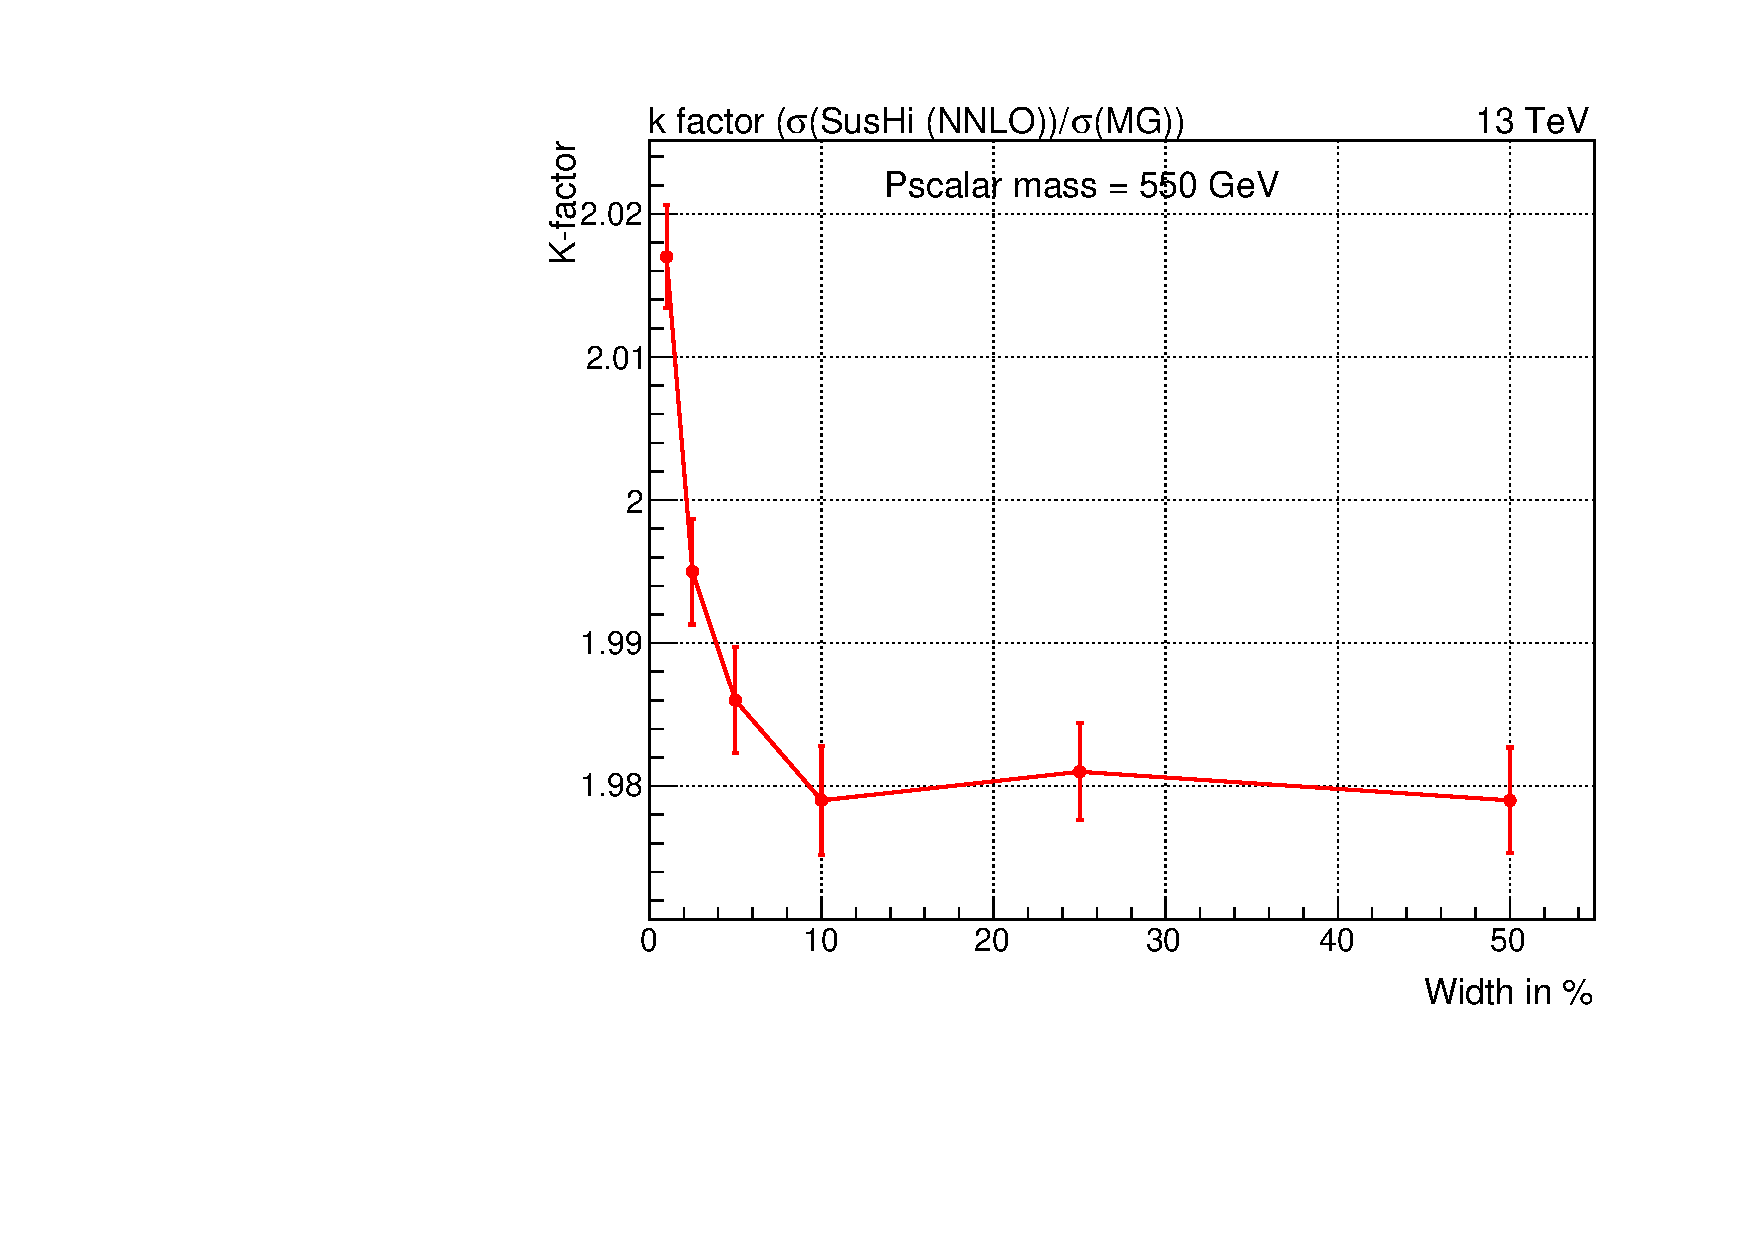
\includegraphics[scale=0.4]{fig/chapt4/k_factor_PScalar_m550_res.pdf}
& \hspace{-0.95cm} 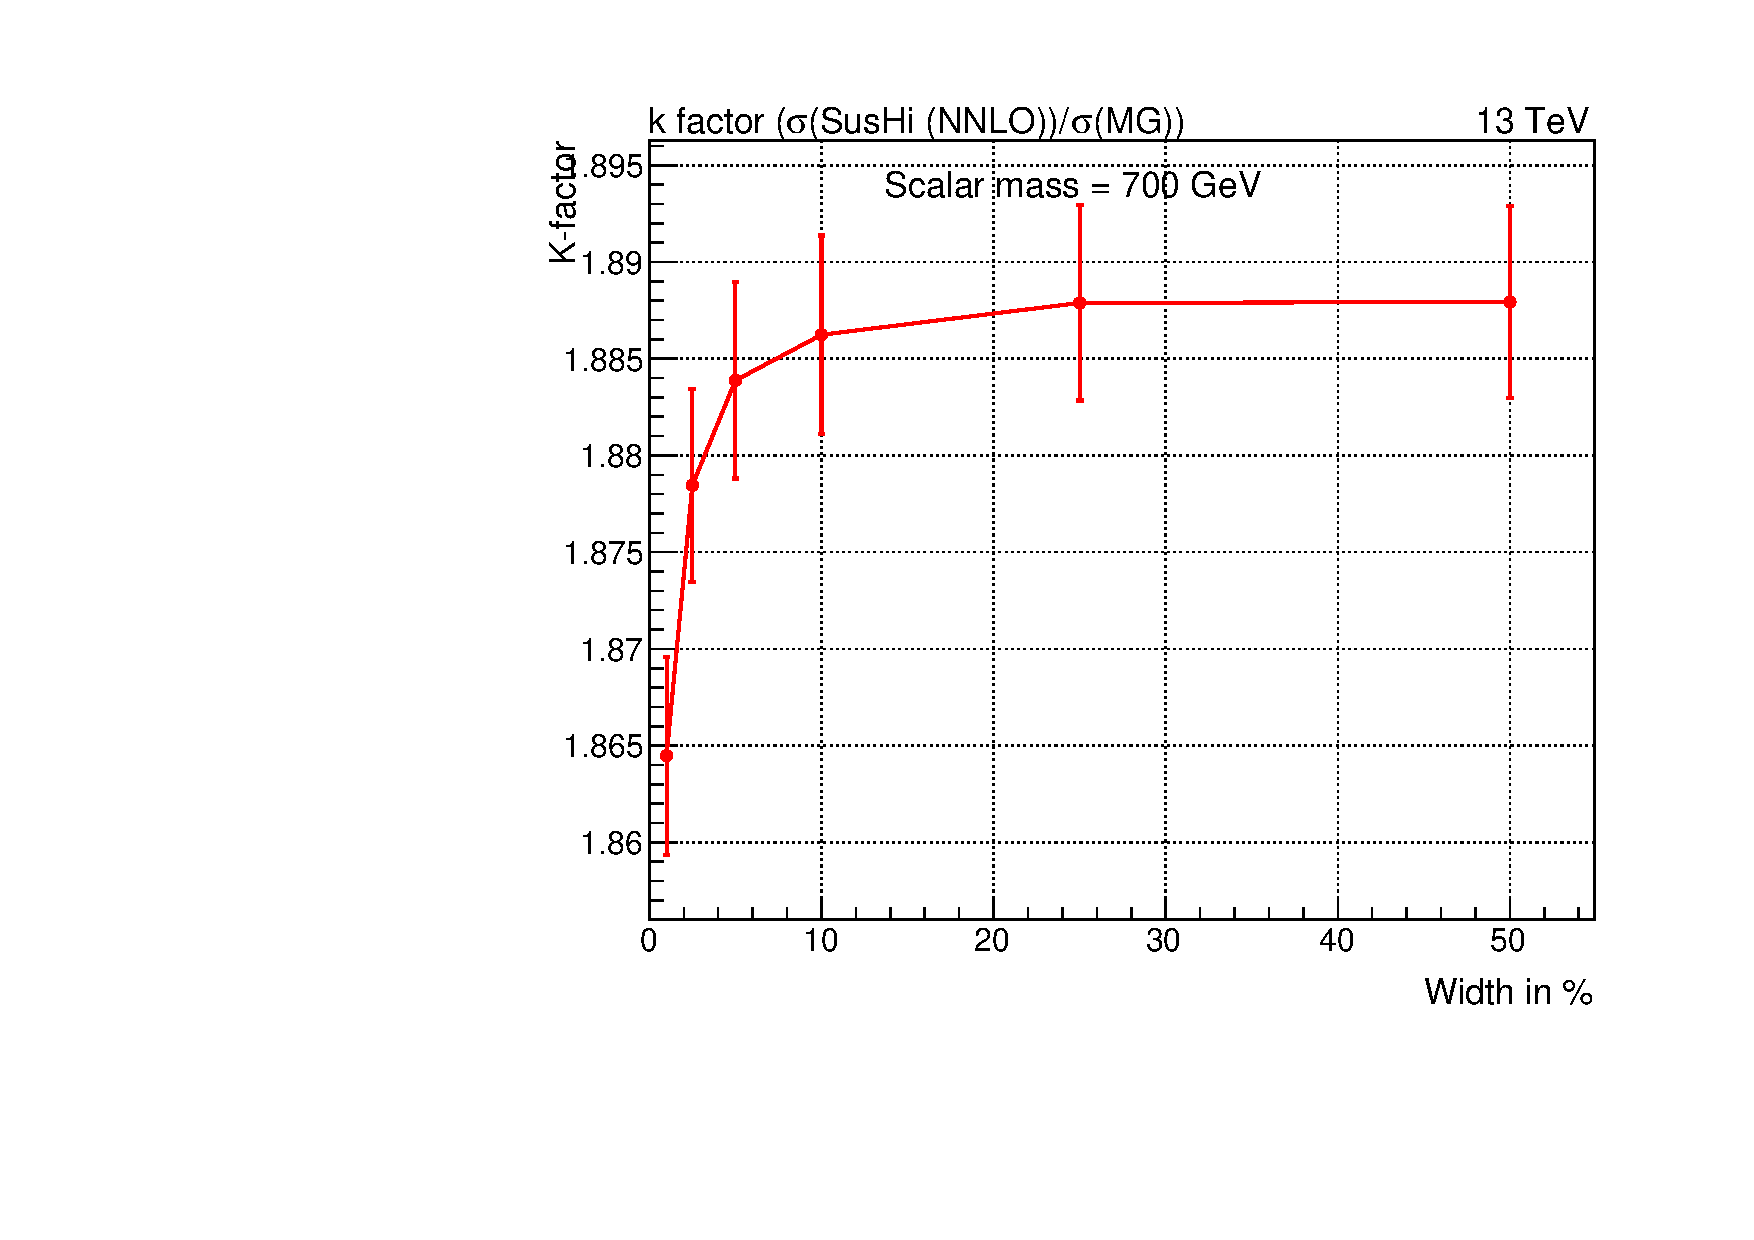
\includegraphics[scale=0.4]{fig/chapt4/k_factor_Scalar_m700_res.pdf}\\
($\mathbf{a}$)\qquad\qquad&($\mathbf{b}$)\qquad\qquad\\ \\
\caption{K-factor for pseudo-scalar mass = 550 GeV (a) and scalar mass = 700 GeV (b), obtained from the ratio of $\sigma_{NNLO}$(SusHi) to $\sigma$(MG). Both SusHi and MG LO cros sections are comparable which gives the same results if we use $\sigma_{LO}$(SusHi) instead of $\sigma_{LO}$(SusHi). For whole range of width, the k-factor shows univesitality which is easy to apply for other values of widths \label{fig:k_factor}.}
\end{tabular}
\end{figure}

\subsection{Top++}\label{subsec:top_pp}
The program Top++ \cite{Czakon:top_pp} calculates the total inclusive cross-section for top pairs production in hadronic collisions using two different approaches a) fixed order with NNLO accuracy and b) including soft-gluon resummation in Mellin space with full next-to-next-to-leading logarithmic order (NNLL) accuracy matched through NNLO. Top++ is the only publicly available program using soft-gluon resummation method for the $t\bar{t}$ inclusive production cross section in hadron colliders.
The program Top++ based on C++ coding in a modular and easy way with a single configuration file ($\texttt{top++.cfg}$) for user interface. The configuration file consists of simple input parameters like, type of collider, pdf set, pure fixed order calculation versus one with resummation, mass of top quark, LO, NLO and NNLO orders. For this work we use top++ to calculate the $t\bar{t}$ hadronic cross section upto NNLO accuracy with soft-gluon resummation and LO cross section without soft-gluon resummation. From these two cross sections, k-factor ($\sigma(NNLO)/\sigma(LO)$) has been calculated for further the scaling of interference. The input parameters used for this study;  


\section{Signal Modelling}\label{sec:signal}
\subsection{Signal Generation and Validation}

    




\clearpage{\pagestyle{empty}\cleardoublepage}

\graphicspath{{chapt_dutch/}{intro/}{chapt2/}{chapt3/}{chapt4/}{chapt5/}{chapt6/}{chapt7/}{chapt8/}}

% Header
\renewcommand\evenpagerightmark{{\scshape\small Chapter 5}}
\renewcommand\oddpageleftmark{{\scshape\small Objects selection and Event Reconstruction}}

\hyphenation{}

\chapter[Physics Objects Selection and Event Reconstruction at CMS]%
{Objects Selection and Event Reconstruction at CMS}
\label{chapt:5}

%****************************************** TESTING DETECTORS UNDER EXTREME CONDITIONS *****************************************************
\section{Physics Objects Reconstruction}\label{sec:Obj_reco}
\subsection{Particle Flow Algorithm}\label{subsec:pfa}
\subsection{Primary Vertex and Track Reconstruction}\label{subsec:pvt}
\subsection{Electron}\label{subsec:electron}
\subsection{Muon}\label{subsec:muon}
\subsection{Jets}\label{subsec:jets}
\subsection{Identification of b-jets}
\subsection{Missing Transverse Energy}\label{subsec:met}
\section{Event Selection}\label{sec:Evnt_selec}
\subsection{Data and Simulated Samples}
\subsection{First Primary Vertex Selection}
\subsection{Noise and Anomalous Events}
\subsection{Tiggers}
\subsection{Leptons}
\subsection{Jets, b-tagging and MET}
\section{Reconstruction of $t\bar{t}$ System}

	


%\renewcommand*{\thesection}{\thechapter.\arabic{section}}       % reset again to chaptnum.sectnum

\clearpage{\pagestyle{empty}\cleardoublepage}

\graphicspath{{chapt_dutch/}{intro/}{chapt2/}{chapt3/}{chapt4/}{chapt5/}{chapt6/}{chapt7/}{chapt8/}}

% Header
\renewcommand\evenpagerightmark{{\scshape\small Chapter 6}}
\renewcommand\oddpageleftmark{{\scshape\small Backgrounds Modelling and Data Driven Techniques for QCD estimation}}

\hyphenation{}

\chapter[Backgrounds Modelling and Data Driven Techniques for QCD estimation]%
{Backgrounds Modelling and Data Driven Techniques for QCD estimation}
\label{chapt:7}

\section{Backgrounds}
\label{sec:bkgs}

\section{Multijet Estimation}\label{sec:multijet}
One of the main background for semi-leptonic $t\bar{t}$ decays is the multijet QCD that has overwhelming cross section. Due to tight selection criteria, only a small fraction of these events mimics the semi-leptonic final state. This requires large simulation samples to have proper QCD modelling and enough statistics after the final selection that is not practical. We used data-driven technique to model our multijet QCD where we defined sideband regions in data that are enriched in QCD events. The distributions of the relevant kinematic variables for fitting taken directly from these data. The mass of $t\bar{t}$ and $cos\theta$* are used as normalization variables. In semi-leptonic decays of $t\bar{t}$, the multijet QCD background can mimic the signal via two main processes.
\begin{itemize}
\item Non-prompt and less isolated leptons from the decay of beauty and charm quarks. These are real leptons that gain significant $p_{T}$ from the mother b and c hadrons and have more activities in the vicinity. Lepton isolation cut suppresses these events.
\item Some hadrons didn't absorbed in the HCAL and make tracks in the muon system or jets with high electromagnetic fraction mimics electron signatures. They are treated as fake leptons.
\end{itemize}
Assuming that the kinematic properties of the multi jet events in selected phase space are independent of the lepton isolation in the event, we reversed the isolation cut to define the control region that is enriched of multijet events and less contamination from other processes. We use following selection criteria for lepton and event.
\begin{itemize}
\item Invert the lepton isolation cut to get enriched multijet QCD events and anti-isolation region is checked in three independent regions.
\item The rest of lepton selection are same as defined in section \ref{Sec:Reconstruction} for both muon and electron.
\item The definition of loose lepton is same as in section \ref{Sec:Reconstruction} but exclude from it the anti-isolated lepton.
\item Jets are cleaned against the isolated leptons.
\item The event is selected if there is at least one anti-isolated lepton where the highest $p_{T}$ lepton is taken into account. The event is rejected if it contains at least a loose lepton.
\end{itemize}
For muon the isolation region is divided according to the isolation variable $I_{rel}^{\mu}(\Delta\beta)$ as in table \ref{table:3Aiso_regions} so that there is a balance between statistical yield and shape compatibility. Comparing shape of data and MC in the three regions, we get enough multijet QCD statistics from simulation shown in figure \ref{Fig:qcd_3region_shapes}. We subtract the expected contribution from non-QCD processes from the data in the three side-band regions shown in figure \ref{Fig:data_driven_qcd}a, b and make pairwise Pearson's $\chi^{2}$ test $H1 \rightarrow Chi2Test(H2, "WW P")$ to find a compatible range for $I_{rel}^{\mu}(\Delta\beta)$. Based on Pearson's $\chi^{2}$ test as in table \ref{table:ch2_results}, we use $0.15 \leq I_{rel}^{\mu}(\Delta\beta) < 0.43$ to obtain the final distributions of $t\bar{t}$ mass and $t\bar{t}$ mass vs cos$\theta$* as shown in figure \ref{Fig:data_driven_qcd}e, f respectively.
We adapt a similar approach for electron channel but with different inverting isolation values for $I(\rho)$ shown in table \ref{table:3Aiso_regions}. The Pearson's $\chi^{2}$ test verified the compatibility for the whole anti-isolation region as in table \ref{table:ch2_results}. The three regions are shown in figure \ref{Fig:data_driven_qcd}c, d using observables $t\bar{t}$ mass and  $t\bar{t}$ mass versus cos$\theta$* respectively. For final fit the two observables shown in figure \ref{Fig:data_driven_qcd}i, j for muon channel and k, l for electron channel, mass of $t\bar{t}$ normalized to its area is used as 1D fit variable and $t\bar{t}$ mass versus cos$\theta$* normalized to its area is used as 2D fit variable projected to 1D.\\
To see the effect of statistical uncertainties on data-driven multijet, we vary the main $t\bar{t}$ background 6\% around the nominal but both up and down variations are consistent shown in the last row of figure \ref{Fig:data_driven_qcd}. For systematics, we studied the main uncertainties from jet energy scale, b-tagging and final state radiation. No effect observed from systematics on data driven multijet QCD.
%------------------------------
\begin{table}[ht]
\caption{Three anti isolation regions for $\mu$ channel and barrel and endcap in electron channel}
\centering
\begin{tabular}{c c c c}
\hline\hline
 & region\#1 & region\#2 & region\#3\\ [0.5ex]
\hline\hline
\multicolumn{4}{c}{$\mu$ channel}\\ \hline
& $0.15 \leq I_{rel}^{\mu}(\Delta\beta) < 0.24$ & $0.24 \leq I_{rel}^{\mu}(\Delta\beta) < 0.43$ & $0.43 \leq I_{rel}^{\mu}(\Delta\beta)$ \\
\hline
\multicolumn{4}{c}{electron channel}\\ \hline
Barrel & $0.0588 \leq I(\rho) < 0.083$ & $0.083 \leq I(\rho) < 0.13$ & $0.13 \leq I(\rho)$\\
Endcap & $0.0571 \leq I(\rho) < 0.083$ & $0.083 \leq I(\rho) < 0.13$ & $0.13 \leq I(\rho)$\\
\hline
\end{tabular}
\label{table:3Aiso_regions}
\end{table}
%------------------------------
\begin{table}[ht]
\caption{Pairwise Pearson's $\chi^{2}$ test values for three anti isolation regions using observables $t\bar{t}$ mass and cos$\theta^{*}$.}
\centering
\begin{tabular}{c c c c}
\hline\hline
 Observable & region 1\&2 & region 1\&3 & region 2\&3\\ [0.5ex]
\hline\hline
 \multicolumn{4}{c}{$\mu$ channel}\\ \hline
$t\bar{t}$ mass & 0.228755 & 1.06025e$^{-80}$ & 2.45163e$^{-94}$ \\
cos$\theta$* & 0.037041 &  4.46683e$^{-33}$& 3.14307e$^{-24}$ \\
\hline
\multicolumn{4}{c}{electron channel}\\ \hline
$t\bar{t}$ mass & 0.778085 & 0.265179 & 0.190154 \\
cos$\theta$* & 0.333658 & 0.115147 & 0.760064\\
\hline
\end{tabular}
\label{table:ch2_results}
\end{table}
%------------------------------
\begin{figure}[htp]
%\centering
\begin{tabular}{ccc}
\hspace{-0.5cm}
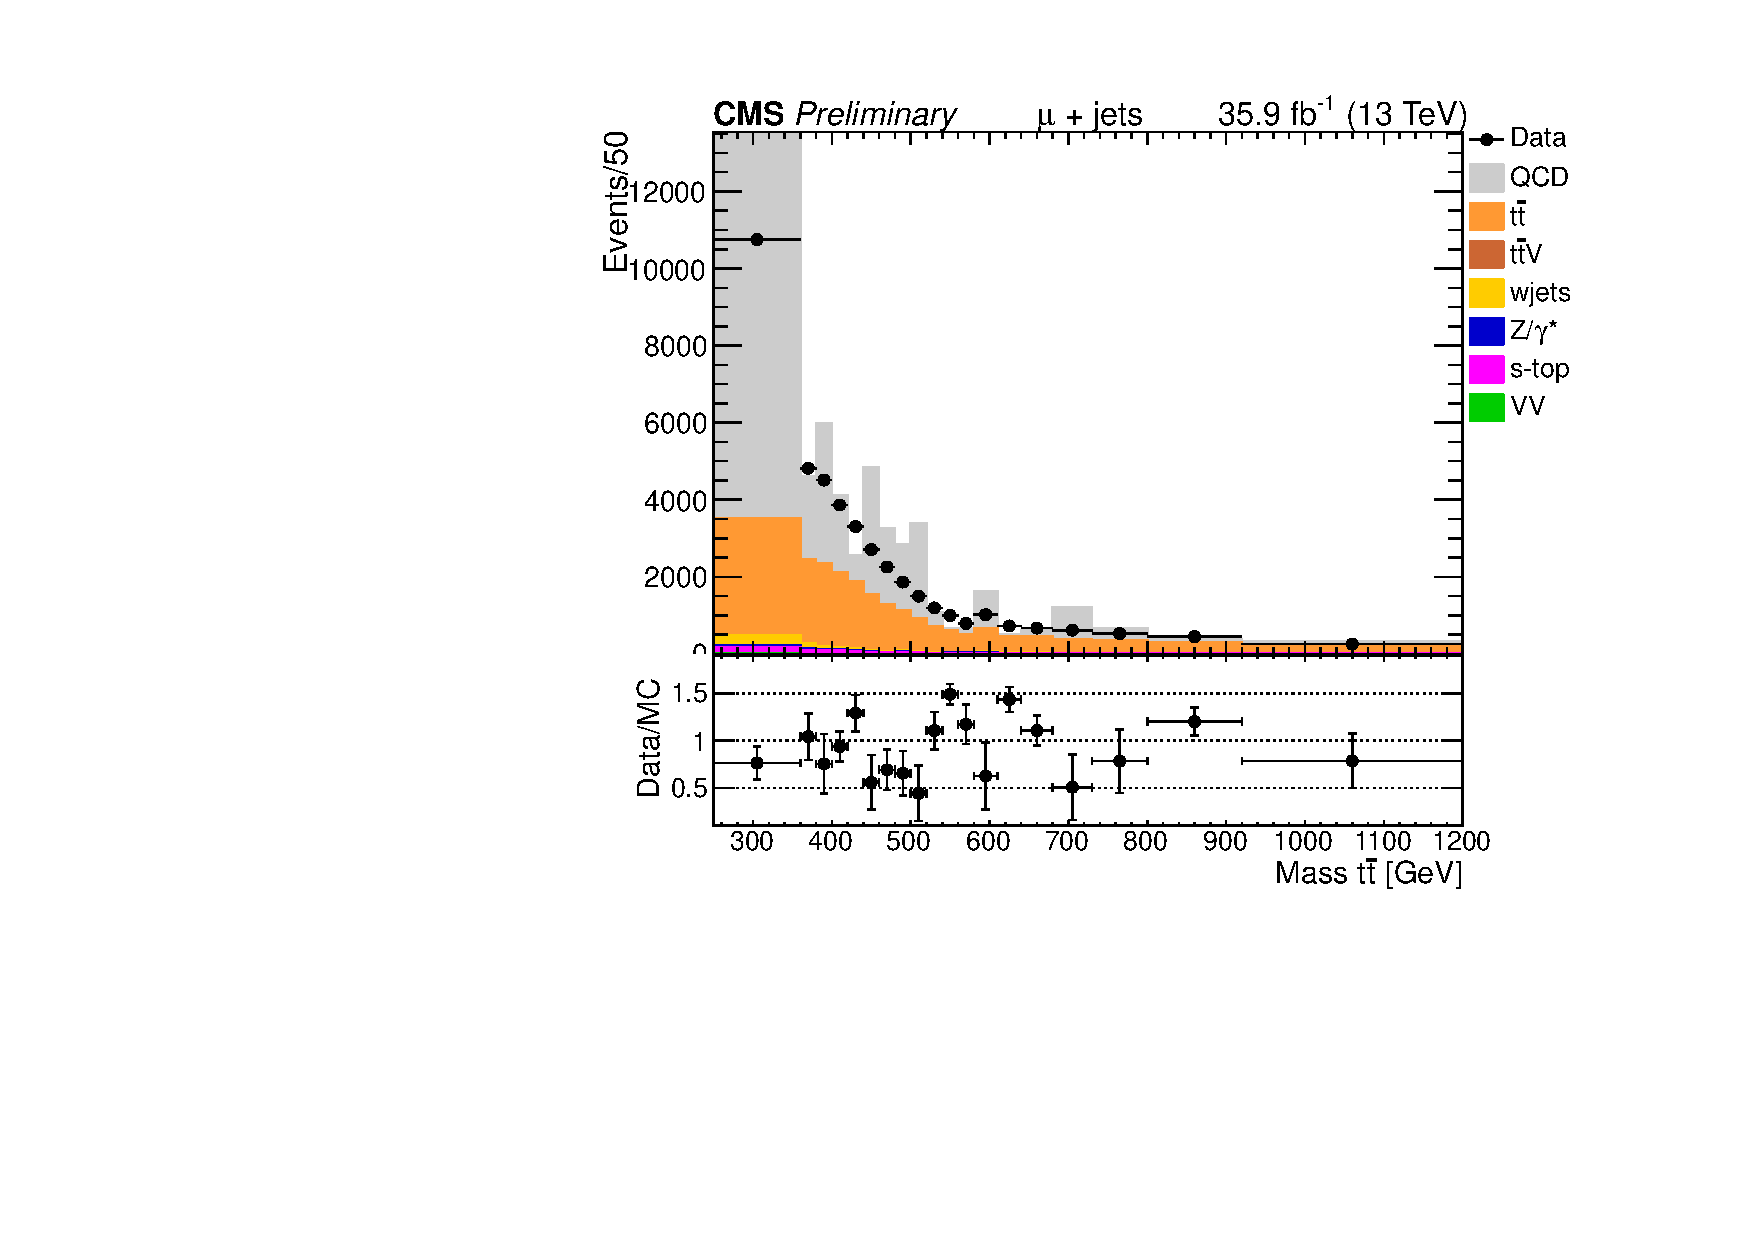
\includegraphics[scale=0.30]{fig/chapt7/qcd/qcd_mu_ch/Mass_H_binned15_24.pdf}
& \hspace{-1.20cm} 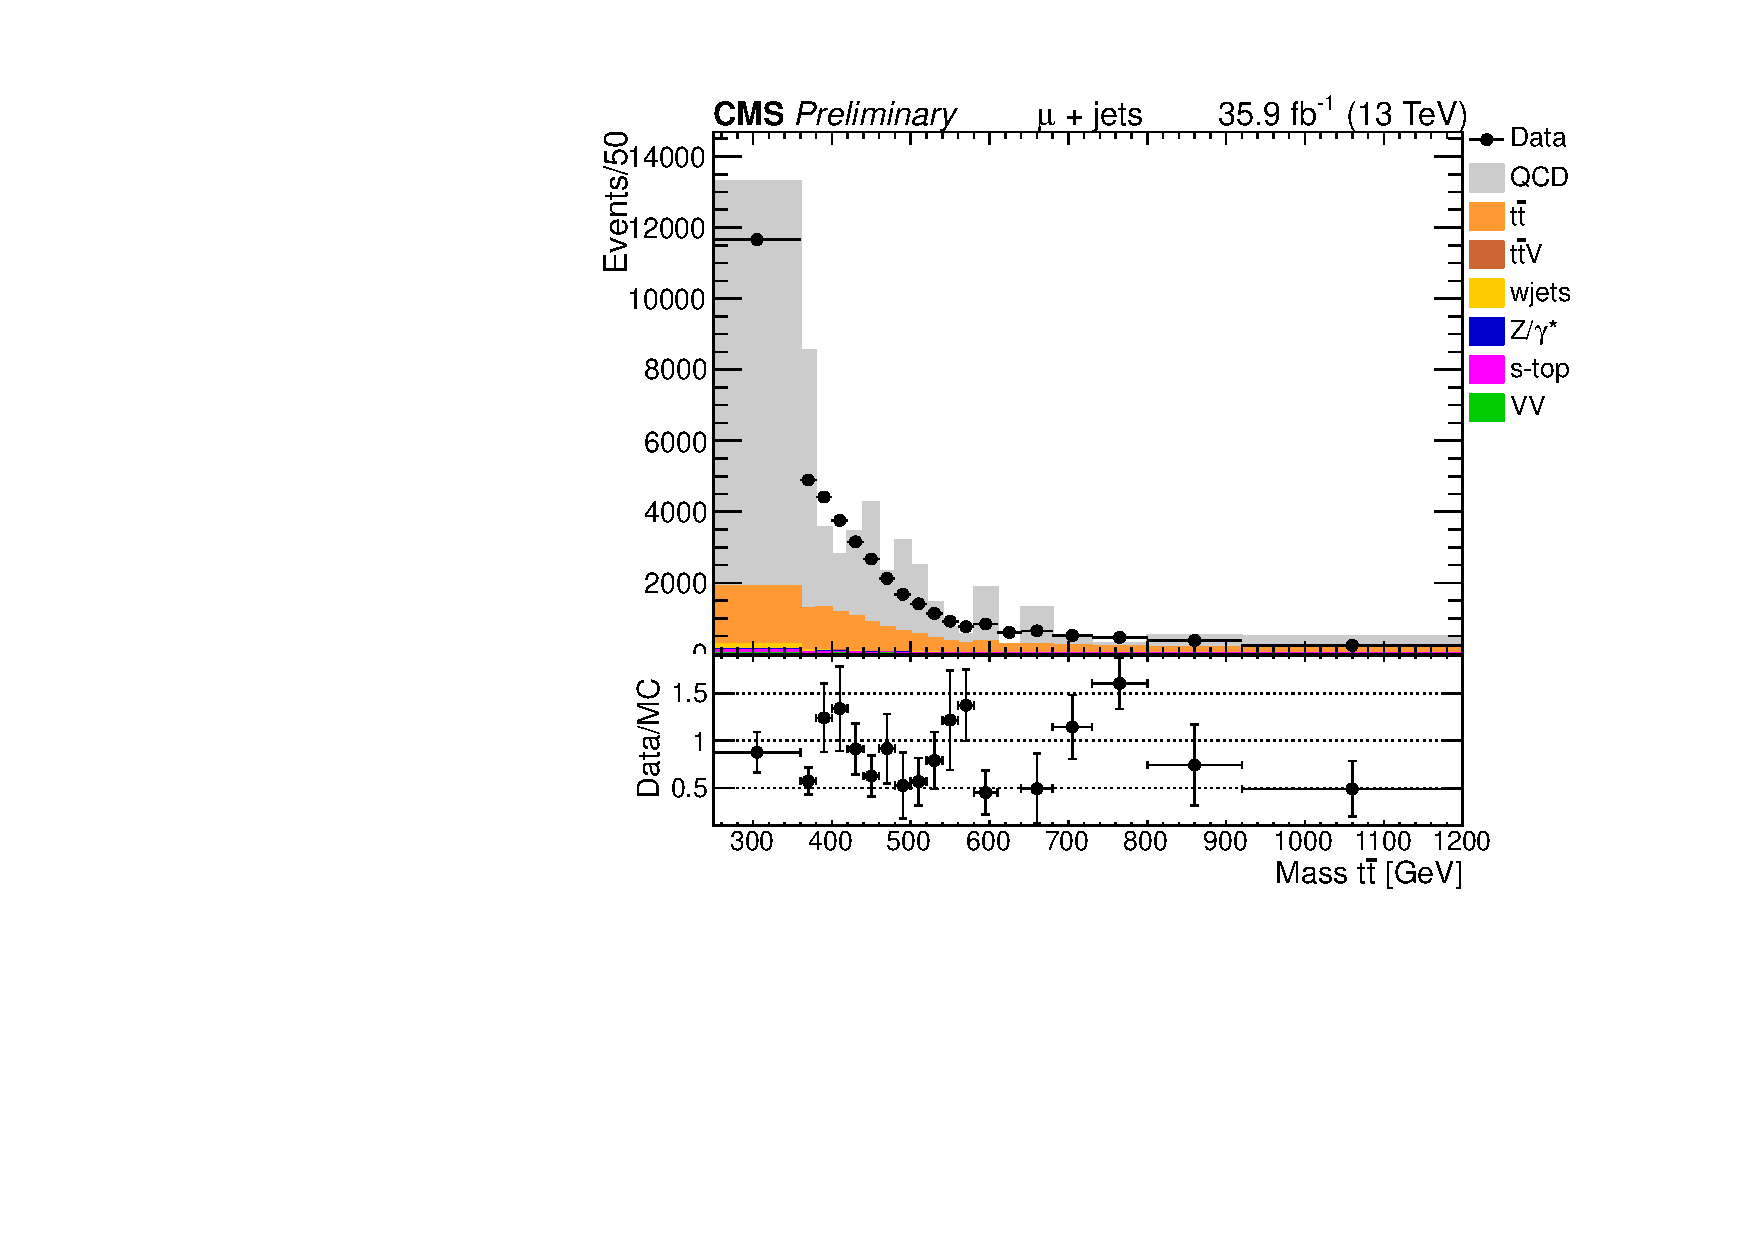
\includegraphics[scale=0.30]{fig/chapt7/qcd/qcd_mu_ch/Mass_H_binned24_43.pdf}
& \hspace{-1.20cm} 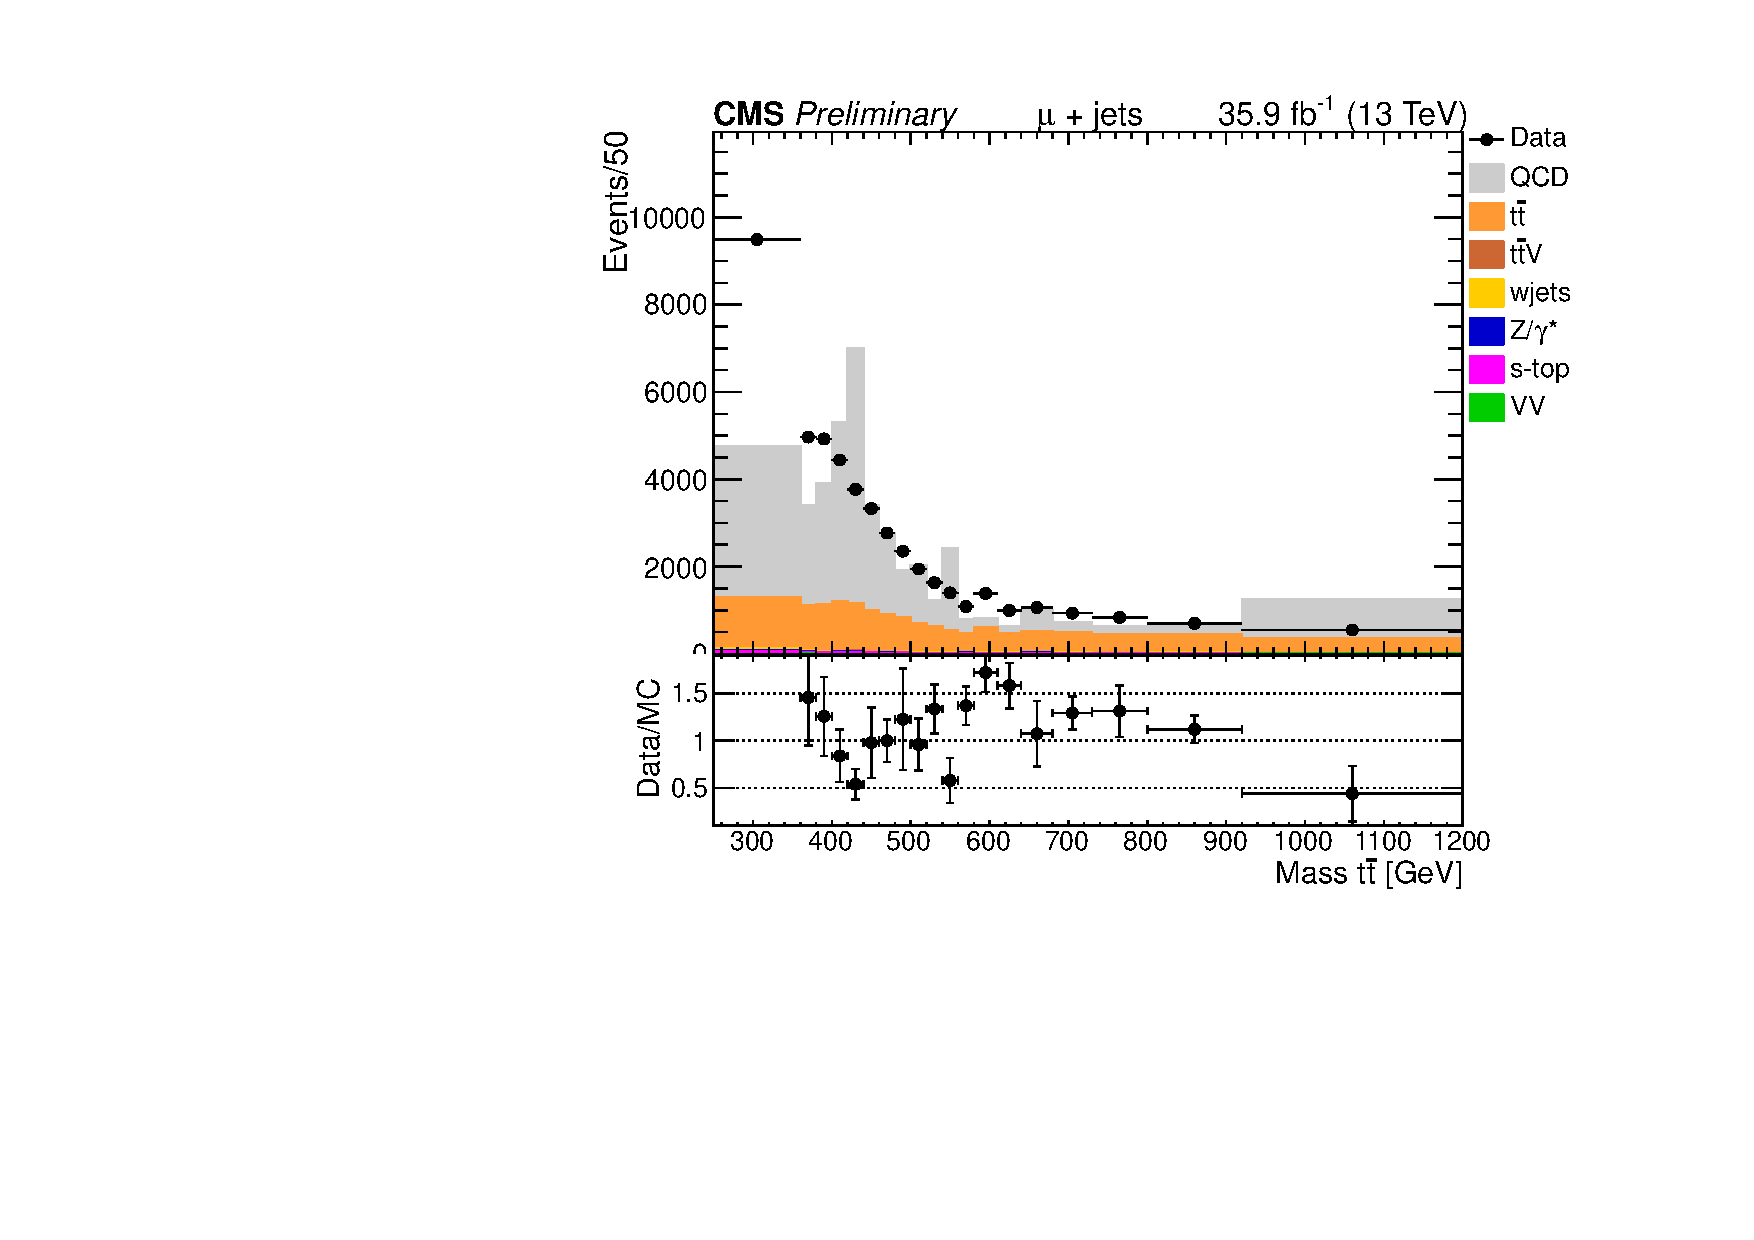
\includegraphics[scale=0.30]{fig/chapt7/qcd/qcd_mu_ch/Mass_H_binned43_Inf.pdf}\\
   ($\mathbf{a}$)\qquad\qquad&($\mathbf{b}$)\qquad\qquad\qquad&($\mathbf{c}$)\qquad\qquad\qquad\\ \\
\hspace{-0.5cm}
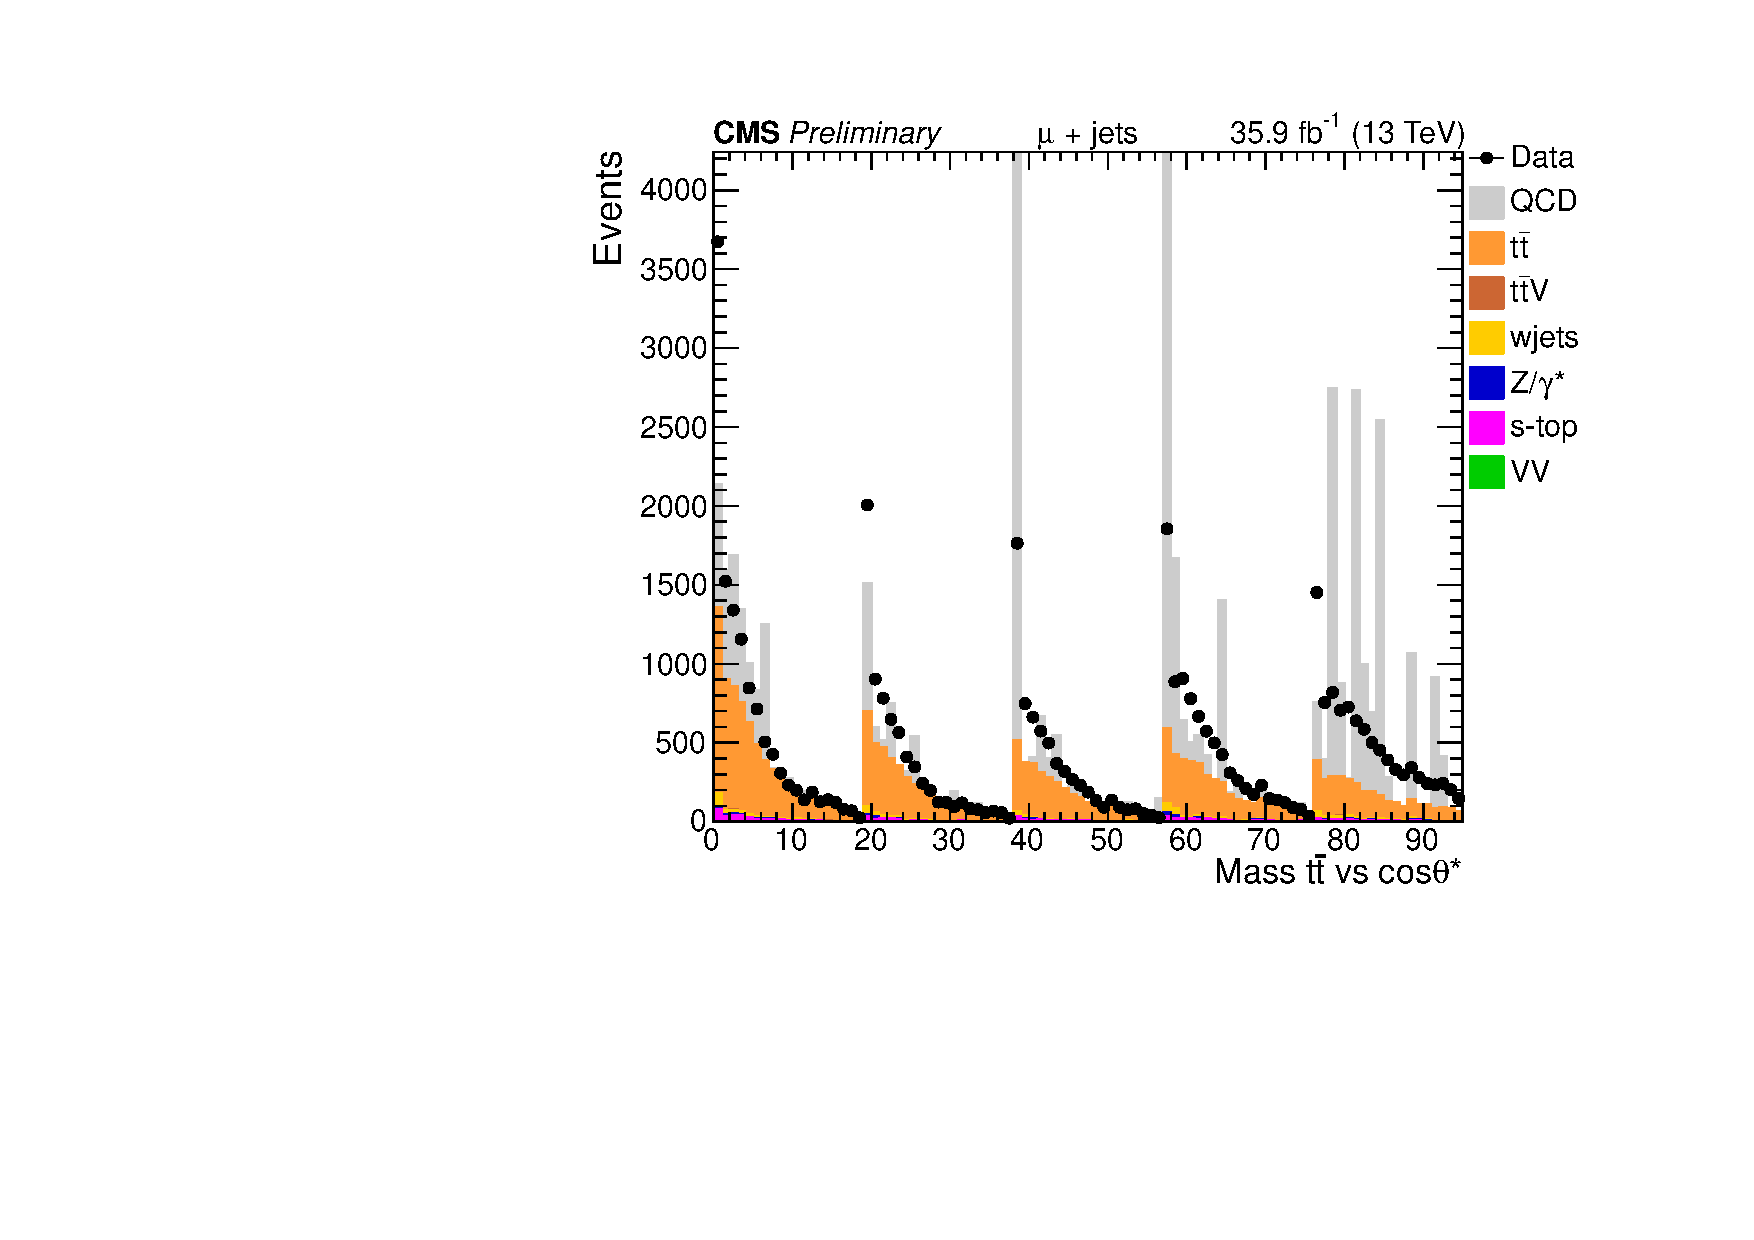
\includegraphics[scale=0.3]{fig/chapt7/qcd/qcd_mu_ch/massH_cos_theta15_24.pdf}
& \hspace{-1.2cm} 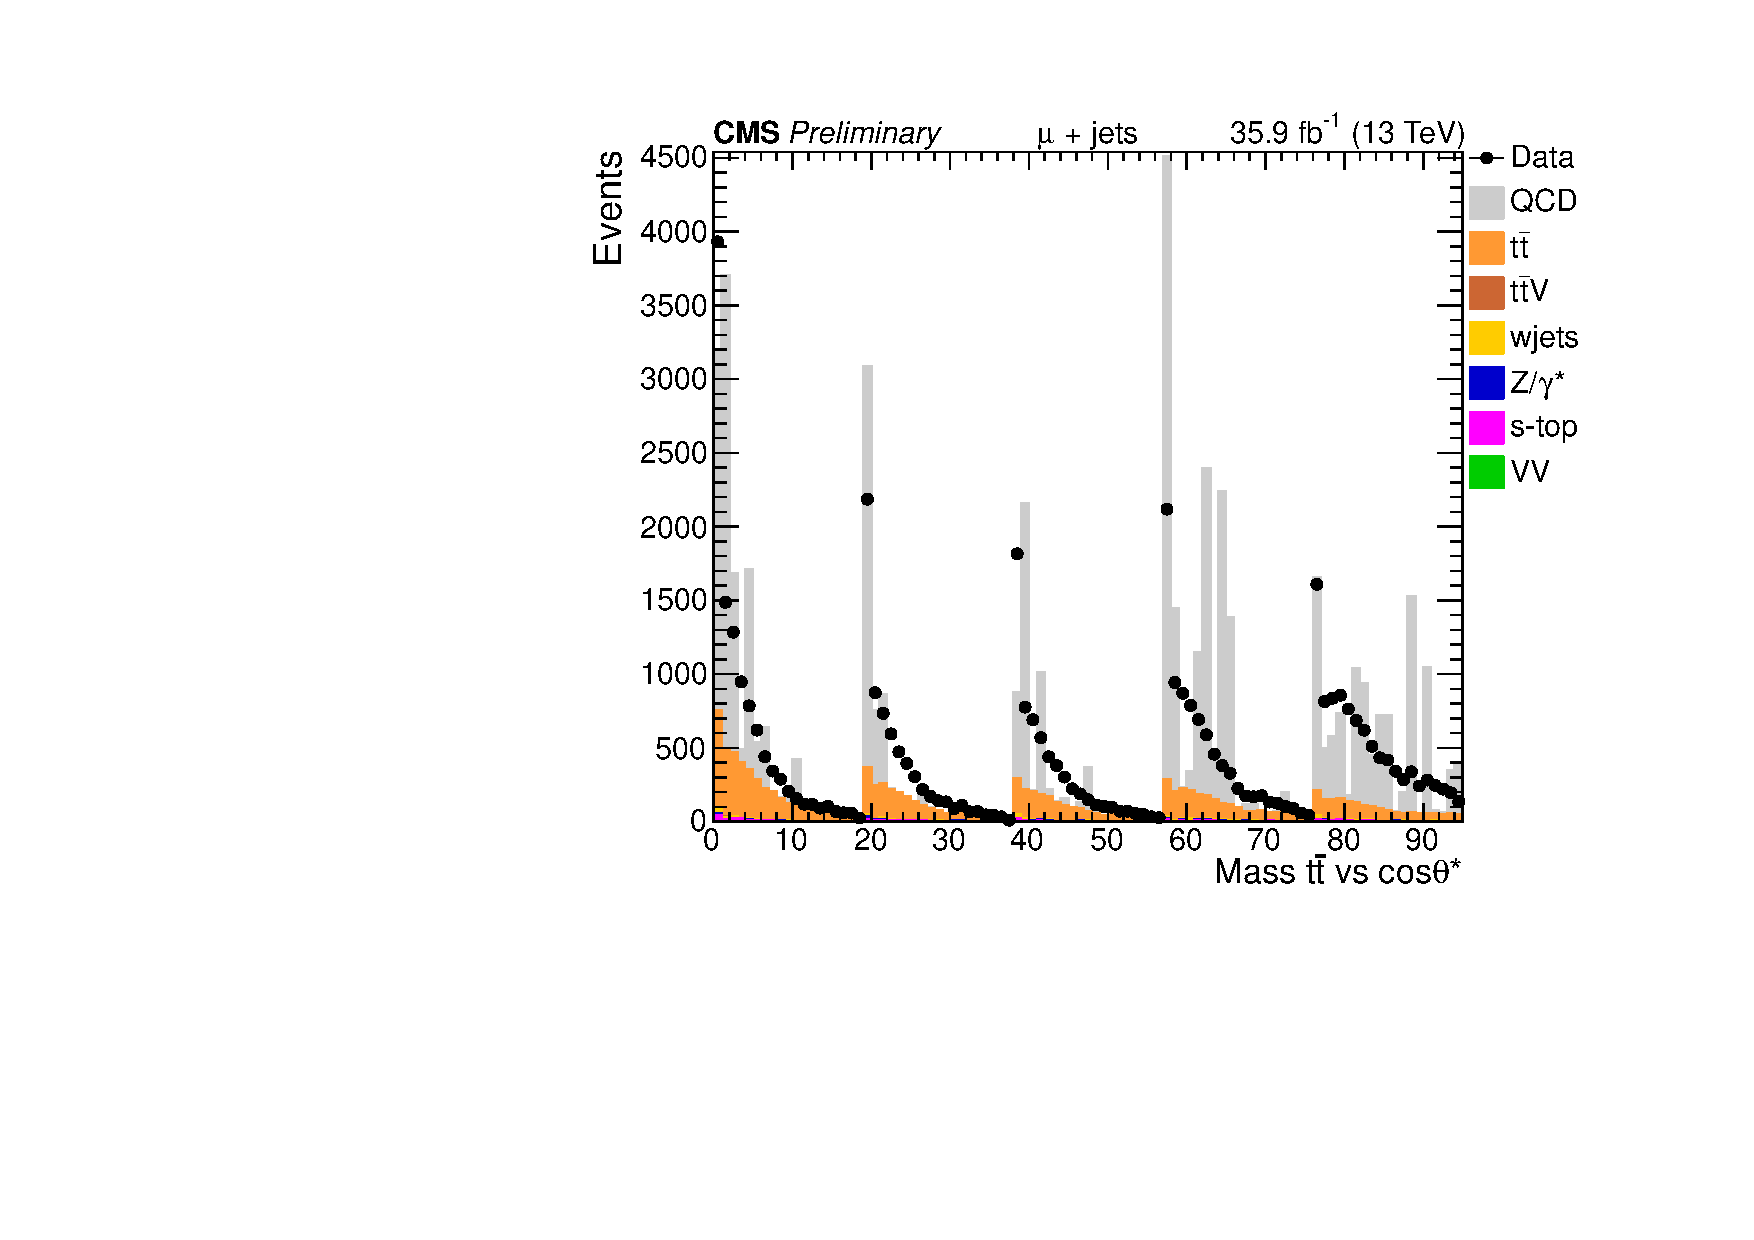
\includegraphics[scale=0.3]{fig/chapt7/qcd/qcd_mu_ch/massH_cos_theta24_43.pdf}
& \hspace{-1.2cm} 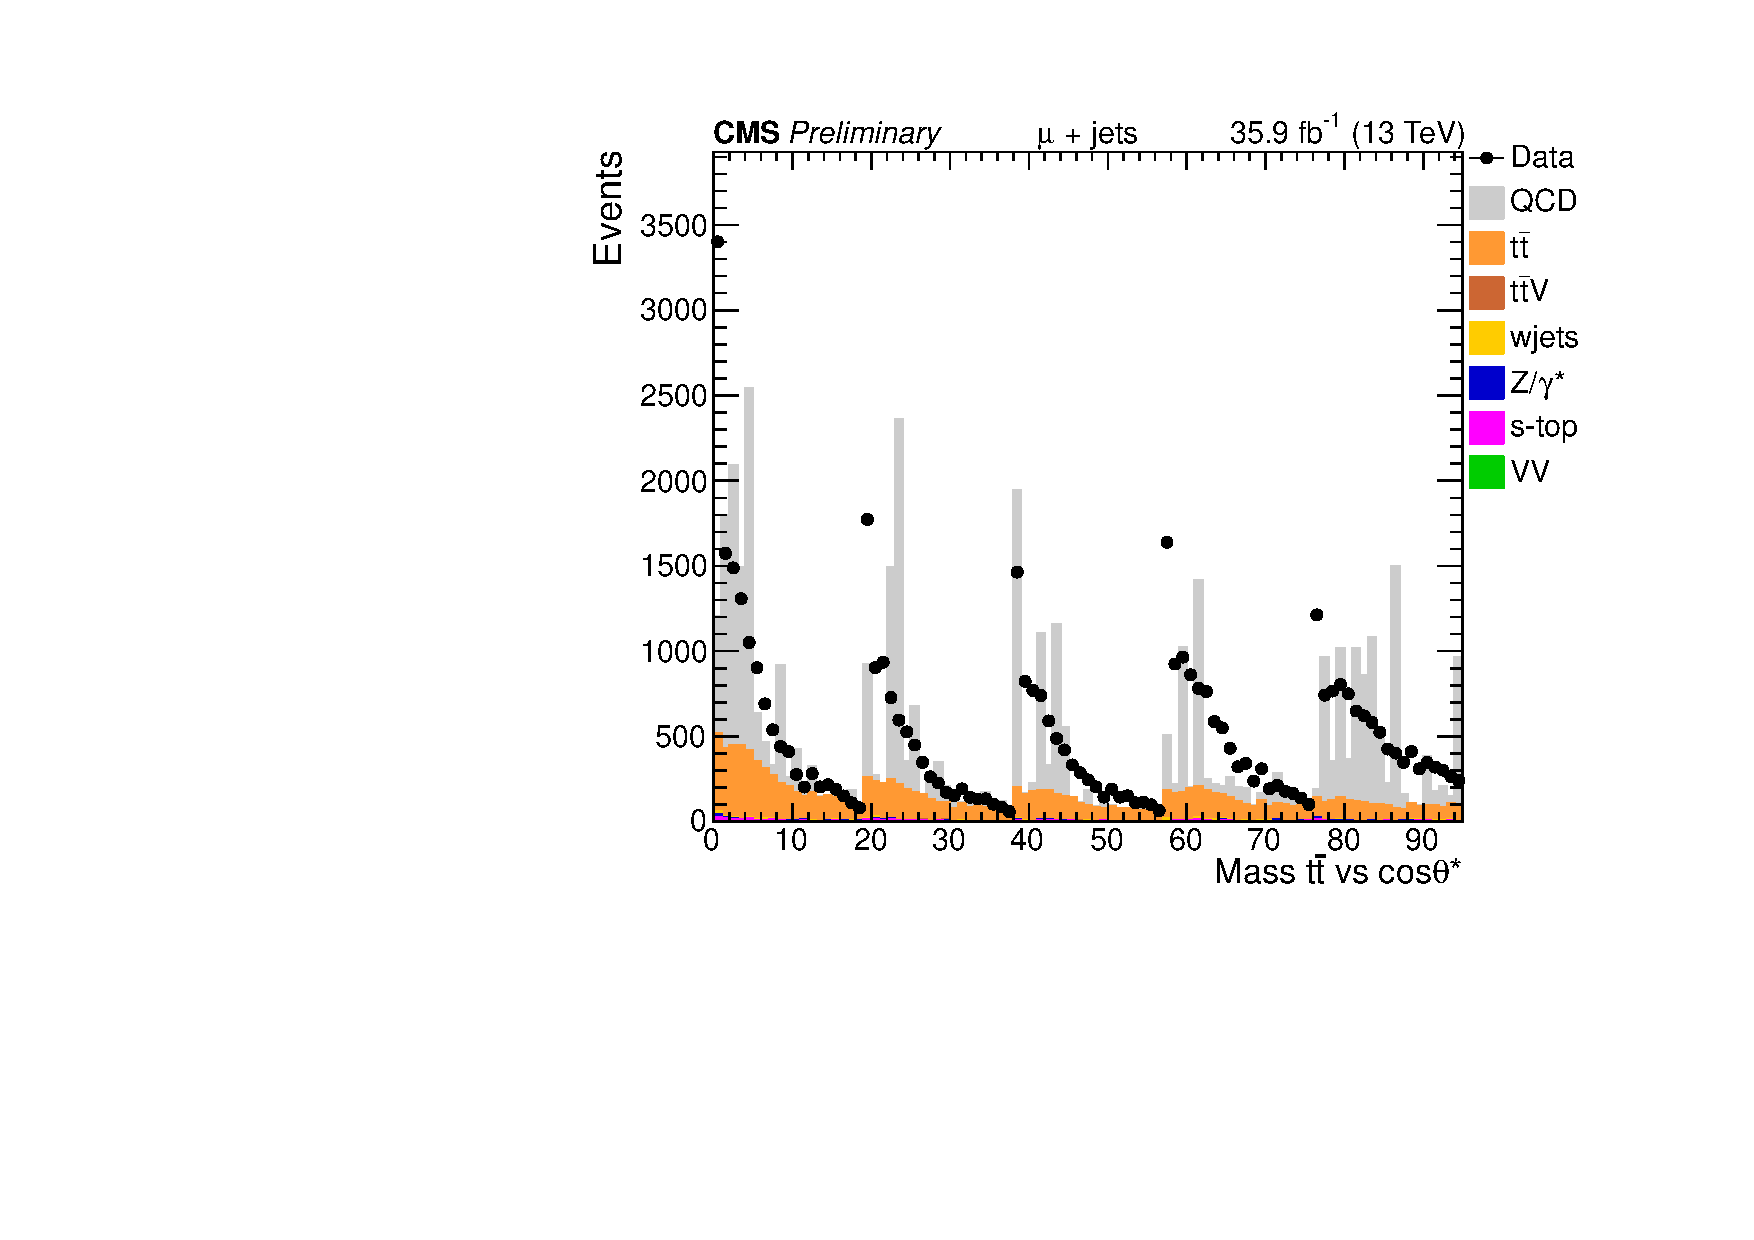
\includegraphics[scale=0.3]{fig/chapt7/qcd/qcd_mu_ch/massH_cos_theta43_Inf.pdf}\\
   ($\mathbf{d}$)\qquad\qquad&($\mathbf{e}$)\qquad\qquad\qquad&($\mathbf{f}$)\qquad\qquad\qquad\\
\hspace{-0.5cm}
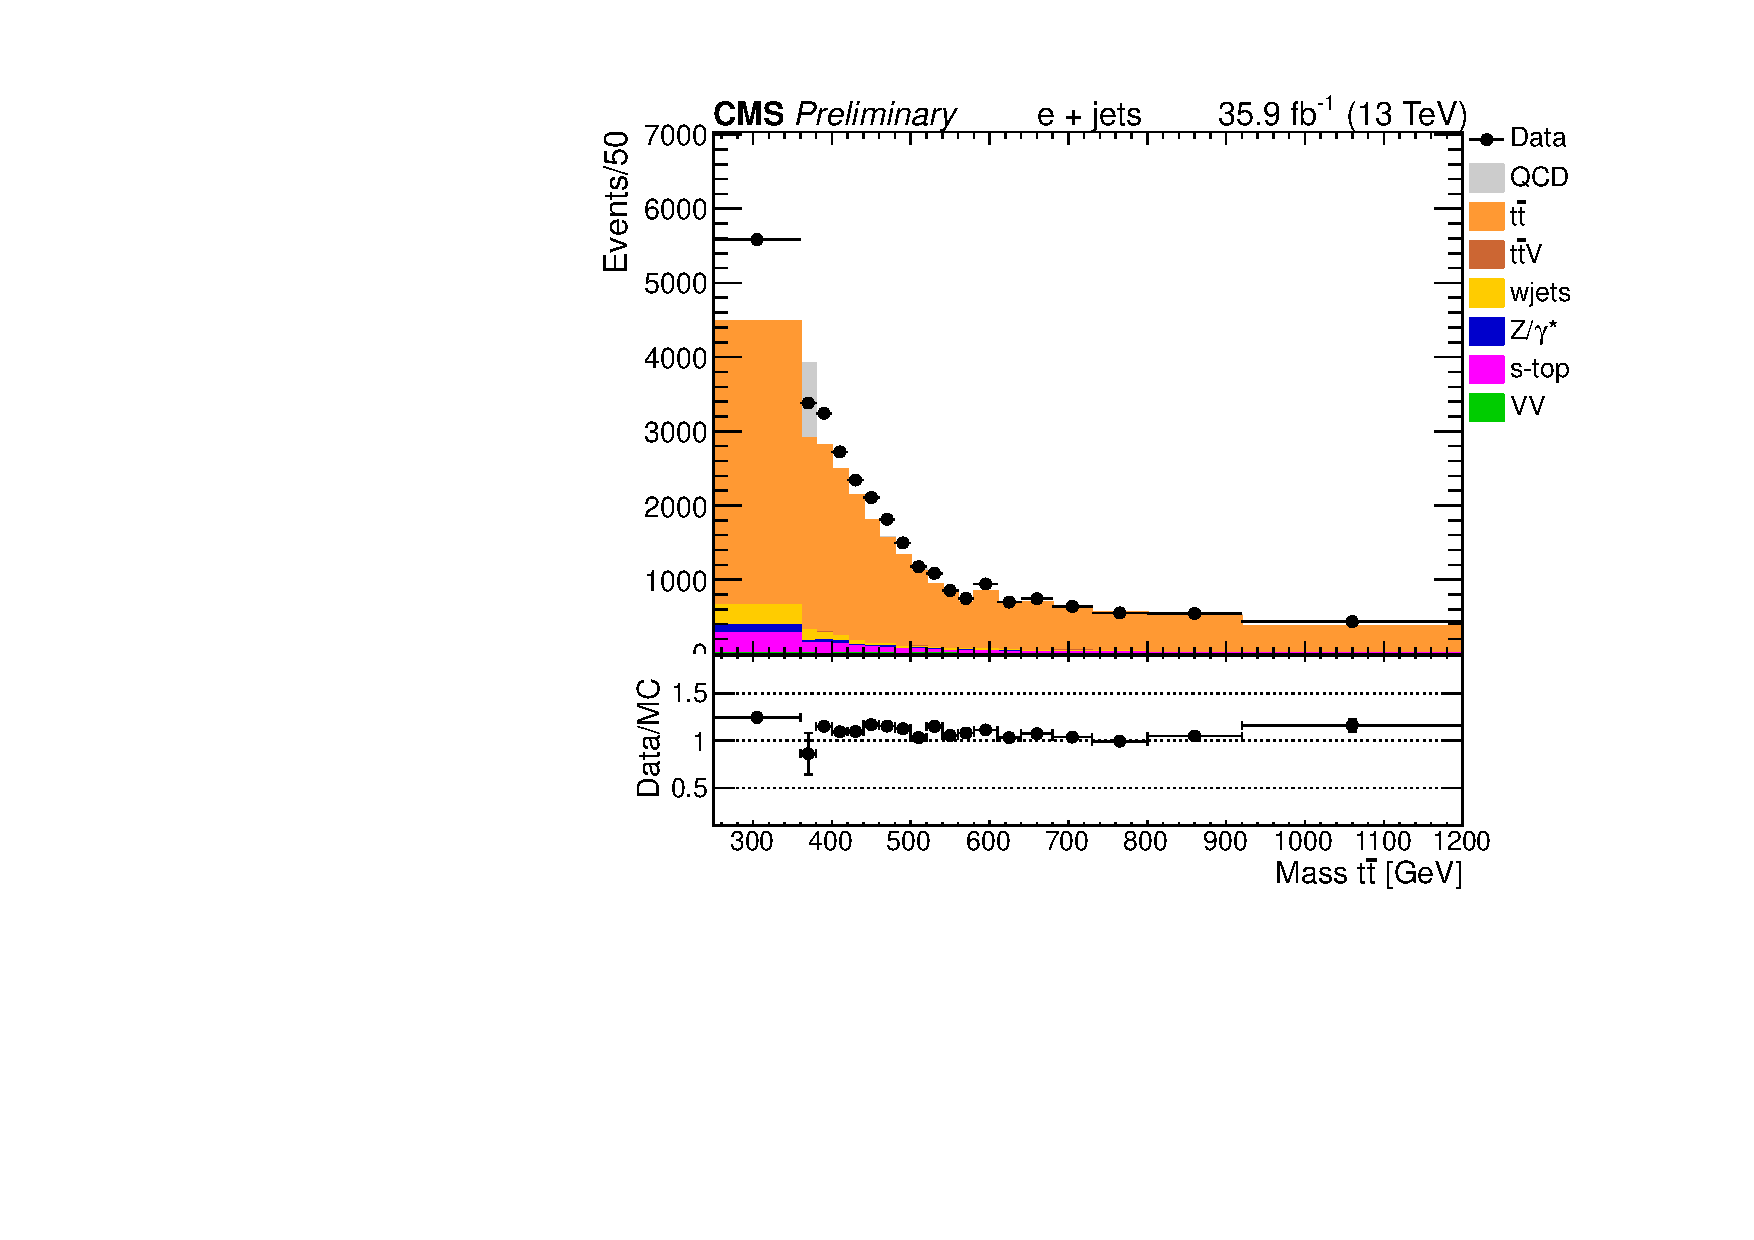
\includegraphics[scale=0.3]{fig/chapt7/qcd/qcd_e_ch/Mass_H_binned1.pdf}
& \hspace{-1.20cm} 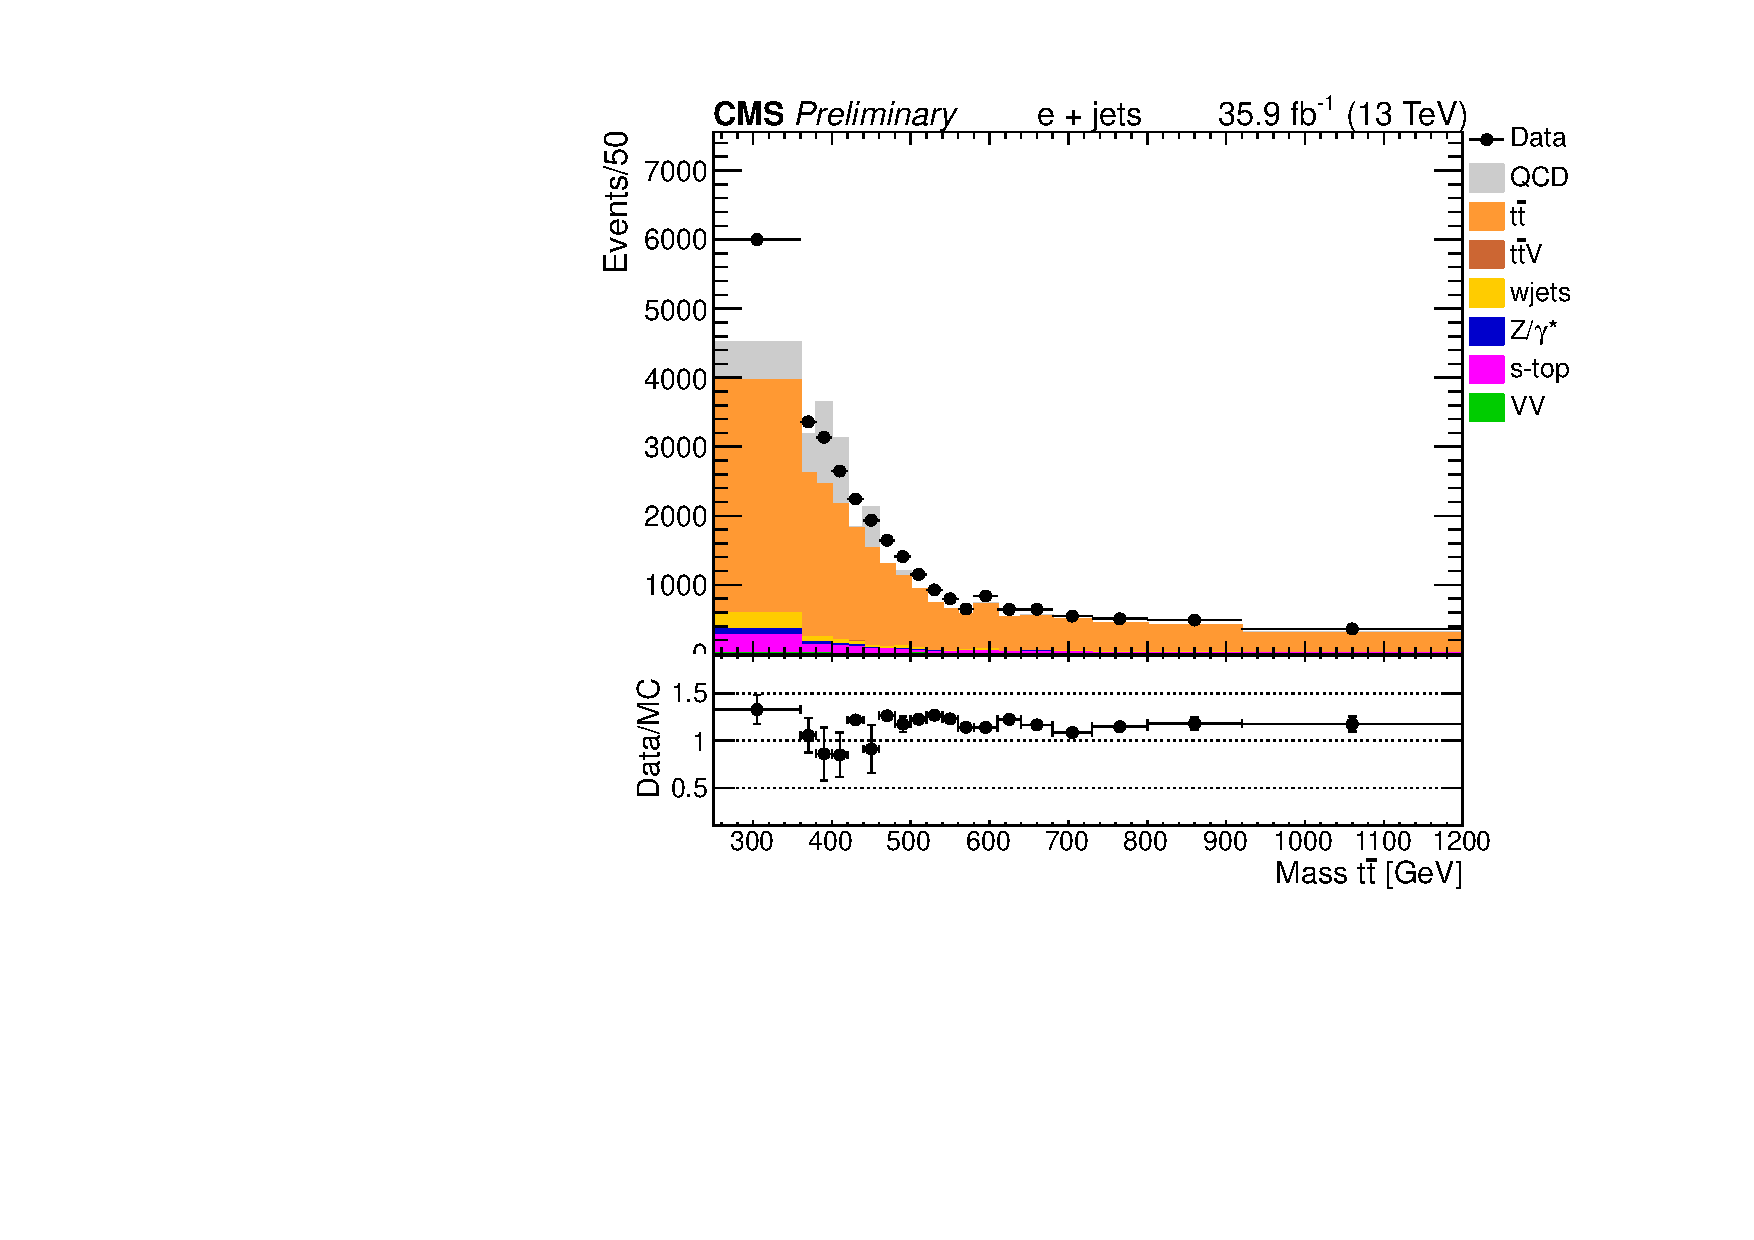
\includegraphics[scale=0.3]{fig/chapt7/qcd/qcd_e_ch/Mass_H_binned2.pdf}
& \hspace{-1.20cm} \includegraphics[scale=0.3]{fig/chapt7/qcd/qcd_e_ch/Mass_H_binned3.pdf}\\
   ($\mathbf{g}$)\qquad\qquad&($\mathbf{h}$)\qquad\qquad\qquad&($\mathbf{i}$)\qquad\qquad\qquad\\ \\
\hspace{-0.5cm}
\includegraphics[scale=0.3]{fig/chapt7/qcd/qcd_e_ch/massH_cos_theta1.pdf}
& \hspace{-1.2cm} \includegraphics[scale=0.3]{fig/chapt7/qcd/qcd_e_ch/massH_cos_theta2.pdf}
& \hspace{-1.2cm} \includegraphics[scale=0.3]{fig/chapt7/qcd/qcd_e_ch/massH_cos_theta3.pdf}\\
   ($\mathbf{j}$)\qquad\qquad&($\mathbf{k}$)\qquad\qquad\qquad&($\mathbf{l}$)\qquad\qquad\qquad\\
\end{tabular}
\caption{Shape comparison of $t\overline{t}$ mass (first row) and $t\overline{t}$ mass versus cos$\theta$* (second row) for Data and MC in $\mu$-channel using three isolation regions: $0.15 \leq I_{rel}^{\mu}(\Delta\beta) < 0.24$ (first column), $0.24 \leq I_{rel}^{\mu}(\Delta\beta) < 0.43$ (second column) and $0.43 \leq I_{rel}^{\mu}(\Delta\beta)$ (last column).\\
For electron channel, third row represents $t\overline{t}$ mass and fourth row $t\overline{t}$ mass versus cos$\theta$* where the isolation regions are: $0.0588 \leq I(\rho) < 0.083$ for barrel and $0.0571 \leq I(\rho) < 0.083$ for endcap in the first column. $0.083 \leq I(\rho) < 0.13$ both for barrel and endcap in the second column and $0.13 \leq I(\rho)$ in third column.}
\label{Fig:qcd_3region_shapes}
\end{figure}
%-----------------------------
\begin{figure}[htp]
%\centering
\begin{tabular}{cccc}
\hspace{-0.5cm}
\includegraphics[scale=0.21]{fig/chapt7/qcd/qcd_mu_ch/cosine_3region_compare.pdf}
& \hspace{-0.95cm} \includegraphics[scale=0.21]{fig/chapt7/qcd/qcd_mu_ch/ttbar_m_3region_compare.pdf}
& \hspace{-0.95cm} \includegraphics[scale=0.21]{fig/chapt7/qcd/qcd_e_ch/cosine_3region_compare.pdf}
& \hspace{-0.95cm} \includegraphics[scale=0.21]{fig/chapt7/qcd/qcd_e_ch/ttbar_m_3region_compare.pdf}\\
($\mathbf{a}$)\qquad\qquad&($\mathbf{b}$)\qquad\qquad&($\mathbf{c}$)\qquad\qquad&($\mathbf{d}$)\qquad\qquad\\ \\
\hspace{-0.5cm}
\includegraphics[scale=0.22]{fig/chapt7/qcd/qcd_mu_ch/Mass_H_binned43_Inf.pdf}
& \hspace{-1.0cm} \includegraphics[scale=0.225]{fig/chapt7/qcd/qcd_mu_ch/massH_cos_theta43_Inf.pdf}
& \hspace{-1.0cm} \includegraphics[scale=0.22]{fig/chapt7/qcd/qcd_e_ch/Mass_H_binned_all.pdf}
& \hspace{-1.0cm} \includegraphics[scale=0.225]{fig/chapt7/qcd/qcd_e_ch/massH_cos_theta_all.pdf}\\
($\mathbf{e}$)\qquad\qquad&($\mathbf{f}$)\qquad\qquad&($\mathbf{g}$)\qquad\qquad&($\mathbf{h}$)\qquad\qquad\\
\\
\hspace{-0.5cm}
\includegraphics[scale=0.22]{fig/chapt7/qcd/qcd_mu_ch/ttbar_m_data_drivenQCD.pdf}
& \hspace{-0.95cm} \includegraphics[scale=0.22]{fig/chapt7/qcd/qcd_mu_ch/ttbar_m_cos_data_drivenQCD.pdf}
& \hspace{-0.95cm} \includegraphics[scale=0.22]{fig/chapt7/qcd/qcd_e_ch/ttbar_m_data_drivenQCD.pdf}
& \hspace{-0.95cm} \includegraphics[scale=0.22]{fig/chapt7/qcd/qcd_e_ch/ttbar_m_cos_data_drivenQCD.pdf}\\
($\mathbf{i}$)\qquad\qquad&($\mathbf{j}$)\qquad\qquad&($\mathbf{k}$)\qquad\qquad&($\mathbf{l}$)\qquad\qquad\\
\\
\hspace{-0.5cm}
\includegraphics[scale=0.22]{fig/chapt7/qcd/qcd_mu_ch/ttbar_m_ttsys_UpDn.pdf}
& \hspace{-0.95cm} \includegraphics[scale=0.22]{fig/chapt7/qcd/qcd_mu_ch/ttbar_m_cosine_ttsysUpDn.pdf}
& \hspace{-0.95cm} \includegraphics[scale=0.22]{fig/chapt7/qcd/qcd_e_ch/ttbar_m_ttsys_6perUpDn.pdf}
& \hspace{-0.95cm} \includegraphics[scale=0.22]{fig/chapt7/qcd/qcd_e_ch/ttbar_m_cosine_ttsys_6perUpDn.pdf}\\
($\mathbf{m}$)\qquad\qquad&($\mathbf{n}$)\qquad\qquad&($\mathbf{o}$)\qquad\qquad&($\mathbf{p}$)\qquad\qquad\\
\\
\end{tabular}
\caption{(a) Shows cos$\theta$* and (b) mass of $t\overline{t}$ for the difference between Data and non-QCD MC in three isolation regions shown in table \ref{table:3Aiso_regions} for $\mu$ channel while (c) and (d) are the same kinematic distributions for electron channel. Distributions (e) and (f) show cos$\theta$* and mass of $t\overline{t}$ vs cos$\theta$* for the range  $0.15 \leq I_{rel}^{\mu}(\Delta\beta) < 0.43$ respectively for muon channel and (g) and (h) for electron channel with $0.0588 \leq I(\rho)$ for barrel and $0.0571 \leq I(\delta\rho)$ in endcap. Third row are the final data-driven multijet QCD distributions normalized to the area and used in fit for statistical evaluation. (i) and (j) are mass of $t\overline{t}$ and mass of $t\overline{t}$ vs cos$\theta$* distributions for $\mu$ channel and (k), (l) for electron channel. A 6\% statistical variation on $t\overline{t}$ is shown is last row for $\mu$ channel in (m), (n) and for electron channel in (o), (p).}\label{Fig:data_driven_qcd}
\end{figure}
%-------------------------------

%\renewcommand*{\thesection}{\thechapter.\arabic{section}}       % reset again to chaptnum.sectnum

\clearpage{\pagestyle{empty}\cleardoublepage}

\graphicspath{{chapt_dutch/}{intro/}{chapt2/}{chapt3/}{chapt4/}{chapt5/}{chapt6/}{chapt7/}{chapt8/}}

% Header
\renewcommand\evenpagerightmark{{\scshape\small Chapter 7}}
\renewcommand\oddpageleftmark{{\scshape\small Corrections to simulation}}

\hyphenation{}

\chapter[Corrections to simulation and systematic uncertainties]%
{Corrections to simulation}
\label{chapt:8}
\section{Corrections to simulation}\label{sec:correc_sim}
\subsection{Pile-up re-weighting}
\label{sec:pileup}

\subsection{Jet Energy Scale}
\label{sec:jes}

\subsection{Jet Energy Resolution}
\label{sec:jer}

\subsection{B tagging}
\label{sec:btag}

\subsection{Trigger, Lepton ID and Isolation}
\label{sec:trig_lepIdIso}

\subsection{Generator level weights}
\label{sec:genweights}

\subsection{Top quark $p_{T}$}
\label{sec:topPt_correc}

\begin{figure}[htp]
\centering
\begin{tabular}{cc}
\hspace{-0.5cm}
\includegraphics[scale=0.45]{fig/correc_uncer/lep_topPT_pdf.pdf}
& \hspace{-1.50cm} \includegraphics[scale=0.45]{fig/correc_uncer/lep_top_ren_fac.pdf}\\
  \qquad ($\mathbf{a}$)\qquad\qquad&($\mathbf{b}$)\qquad\qquad\qquad\qquad \\
\end{tabular}
\caption{ }\label{fig:top_pt_correc_expec}
\end{figure}

\section{Systematic uncertainties}\label{sec:sys_unc}
\subsection{Luminosity}
\label{sec:syslumi}

\subsection{Pileup}
\label{sec:syspileup}

\subsection{Jet energy scale}
\label{sec:sysjes}

\subsection{Jet energy resolution}
\label{sec:sysjer}

\subsection{Unclustered MET}
\label{sec:sysmet}

\subsection{b-tagging and misidentification efficiencies}
\label{sec:sysbtag}

\subsection{Lepton trigger/isolation/identification efficiencies}
\label{sec:systrigg}


%\renewcommand*{\thesection}{\thechapter.\arabic{section}}       % reset again to chaptnum.sectnum

\clearpage{\pagestyle{empty}\cleardoublepage}

\graphicspath{{chapt_dutch/}{intro/}{chapt2/}{chapt3/}{chapt4/}{chapt5/}{chapt6/}{chapt7/}{chapt8/}}

% Header
\renewcommand\evenpagerightmark{{\scshape\small Chapter 8}}
\renewcommand\oddpageleftmark{{\scshape\small Detector Control System for RPCs at GIF++}}

\hyphenation{}

\chapter[Detector Control System for RPCs at GIF++]%
{Detector Control System for RPCs at GIF++}\label{chapt:10}

\section{Introduction}\label{sec:gif_intro}
The High Luminosity Large Hadron Collider (HL-LHC) machine will induce higher background radiations compared to the current operating conditions. It is important to study the performance and stability of the currently installed and future detectors in a high radiation environment. Focused on these requirements, the CERN Engineering- (EN) and Physics- Department (PH) made a joint project, the Gamma Irradiation Facility (GIF++) \cite{JAKEL2014}. GIF++ is the new CERN irradiation facility located in the North Area of the CERN Super Proton Synchrotron (SPS). It is a unique place where high energy ($\sim$100 GeV) charged particles (mainly muons) are combined with a high flux of gamma radiation (662 keV) produced by 13.9 TBq $^{137}$Cs source . An attenuator system is installed to vary the gamma flux on the two sides of the source independently. A schematic overview of the GIF++ is shown in figure \ref{fig:gif}.\\
The Compact Muon solenoid (CMS) is one of the two general-purpose detectors at the LHC \cite{cms-lhc}, which uses Resistive Plate Chambers (RPCs) along with other detectors \cite{muon-sys} for the muon detection. In April 2015, the RPC detectors were installed at the GIF++ to study the performance at a radiation dose equivalent at 3000 fb$^{-1}$ of the CMS. A dedicated control system has been built to control these detectors and archive the relevant parameters using the WinCC-OA (PVSS) Supervisory Control And Data Acquisition (SCADA) system \cite{twiki:wincc-oa}. The system controls high voltage and low voltage supplies and monitors temperature, pressure and humidity of both the RPC gas and the environment. The source status and attenuator values are accessed through the Data Interchange Protocol (DIP), published centrally by the Engineering Department. The RPC gas supply is controlled and monitored by an external WinCC-OA project, that shares relevant parameters with this project. All relevant parameters are archived in a Structured Query Language (SQL) database (DB) for offline analysis.\\
One of the features of the GIF++ RPC DCS system is accessing the source status and attenuator values. Based on this information, RPC performance parameters (efficiency, working point, cluster size and resistivity) are measured. To retrieve the data from the database, a specific algorithm has been developed to synchronize the detector parameters (current and voltage) with the external parameters (temperature, pressure and humidity). It enables to monitor precisely the effect of external parameters on the detector.
\begin{figure}[H]
\centering
\hspace{-0.5cm}
\includegraphics[scale=0.35]{fig/wincc/GIF.png}
 \caption{An overview of the GIF++.}
\label{fig:gif}
\end{figure}
\section{Motivation}\label{sec:gif_motiv}
At HL-LHC, RPCs and associated electronics will operate at much higher luminosity ($\sim$ 5 $\times$ 10$^{34}$ cm$^{-2}$ s$^{-1}$) while accumulating large radiation dose expected from more than 3000 fb$^{-1}$. A precise understanding of the ageing of detector's material and currently installed electronics is needed in intensively high radiation. 
The GIF++ gives the same conditions which will be present at CMS during HL-LHC. The RPCs are irradiated with photons, produced by a $^{137}$Cs radiation source of 13.9 TBq.  At the same time, a high-momentum-particles beam extracted from the SPS, mainly consist of muons, is used to study the performance of the detectors by measuring and comparing their efficiency. The two main gas components of the RPC detector are C$_{2}$H$_{2}$F$_{4}$ and SF$_{6}$ which are going to be gradually banned due to greenhouse effects. An R\&D of different gases mixture is under study at GIF++ to replace the two gases by eco-friendly gases. When a good candidate for a new RPC gas mixture is identified, the study will be further carried out at GIF++ to include long-term assessment of the radiation tolerance of the chambers operated with the new gas mixture. Further details can be found in \cite{phase2}.

\section{WinCC-OA}\label{sec:wincc}
Large experiments at CERN use WinCC-OA as a tool to develop control systems. It allows for the description of a device in terms of a data point, with data point elements representing its parameters. These can then be addressed directly to write to and read from the corresponding device. Parameters of interest can then be stored by WinCC-OA in an internal database for offline analyses. WinCC-OA provides the facility to build a graphical user interface (GUI).

\section{The CMS RPC DCS project at GIF++}\label{sec:rpc_proj}
The CMS RPC DCS at GIF++ has been developed by using WinCC-OA 3.11 and extended with the standard Joint Control Project (JCOP) framework \cite{jcop}. The JCOP framework provides extra functions such as standardized Finite State Machine (FSM), the additional Graphical User Interface (GUI), the alarm handlers and the ORACLE database interface \cite{g-polese}. The high voltage and low voltage power supplies used in the RPC GIF++ setup consist of CAEN SY1527 mainframe modules as well as CAEN EASY modules, with additional ADC modules used to read out gas and environmental sensors (pressure, temperature and humidity). The project has access to the hardware registered through an Object Linking and Embedding (OLE) for Process Control (OPC) server provided by CAEN using the OPC protocol \cite{opc}. The project controls the high voltage and low voltage system through the OPC protocol. The environmental and gas sensors ( for pressure, temperature and humidity) are also readout via the OPC protocol. The source status and attenuator values are available centrally via the Data Interchange Protocol (DIP). The project has been designed as a distributed one in order to be able to communicate with other projects and to read valuable information. Communication has been established with the central GIF++ DCS, such that the information from the gas system, like flow rates are readable.\\
The Finite State machine (FSM) hierarchy of the project is based on the naming convention of the trolley, where the detectors are installed. Each trolley has six sections and each section accommodates one detector. Currently three CMS RPCs trolleys are installed in the GIF++. Trolley 1 (RPC Consolidation) is equipped with spare RPCs, trolley 2 with small glass RPCs and trolley 3 with prototypes of improved RPCs. Detailed information of the trolleys are given here \cite{salvador}. 
A schematic overview of the DCS project is shown in figure \ref{fig:DCS_sys}.
\begin{figure}[H]
\centering
\hspace{-0.5cm}
\includegraphics[scale=0.4,trim=60 30 60 30,clip]{fig/wincc/DCS_sys.png}\\
 \caption{DCS project overview.}
\label{fig:DCS_sys}
\end{figure}

\subsection{High and Low Voltage System}
The high and low voltage system is controlled and monitored through the CAEN OPC server. Each gap of a chamber is independently connected to a single high voltage channel which improves the granularity of control. The RPC front-end electronics requires digital and analog power supplies \cite{feb}. Each low voltage line has been shared between two front-end-boards (FEBs) for digital as well as for analog. The low voltage boards are installed in the CAEN main frame and controlled by DCS.

\subsection{Environmental and Gas Parameters}
The performance of RPCs strongly depends on the temperature and pressure of the environment. Hence, it is important to measure the environmental parameters (temperature, pressure and humidity) at different locations. The applied voltage is corrected for the environmental temperature and pressure in order to include its effects. This procedure is described in detail in \cite{env-rpc}.  
Figure \ref{scan_temp}a gives a plot for environmental temperature, pressure and humidity. The environmental and gas sensors (temperature, pressure and humidity) are readable through ADC (analog-to-digital converter) board which is installed in the EASY crate. The JCOP framework gives the opportunity to convert online the ADC counts into physical values. The trending feature provides a comparison among different sensors located at different positions.

\subsection{High Voltage Scan and Stability Test}
The project has been designed for R\&D of detectors, hence, should be able to perform high voltage scanning or stability tests. For high voltage scanning, a separate branch has been incorporated in the Finite State Machine (FSM) tree, where the user operates each detector independently. The stability test runs for long time. Based on the requirements, a dedicated manager is used to apply the stability script and restart it automatically. A high voltage scanning plot for one of the CMS RPC chambers (RE3) at GIF++ is shown in figure \ref{scan_temp}b. 

\begin{figure}[htp]
\centering
\begin{tabular}{cc}
\hspace{-0.3cm}
\includegraphics[scale=0.25,trim=50 70 20 90,clip]{fig/wincc/tprh.png}
& \hspace{-0.5cm} \includegraphics[scale=0.26,trim=50 100 45 80,clip]{fig/wincc/HV_Scan2.png}\\
   ($\mathbf{a}$)\qquad&($\mathbf{b}$)\qquad\\
\end{tabular}
\caption{(a): Environmental temperature ($^o$C), pressure (mb) and humidity (\%). Time is on x-axis while red, blue and green lines show the values of pressure, temperature and humidity respectively on y-axis. Pressure and temperature values used for operating voltage correction of RPCs. (b): A high voltage scan for CMS RE3 chamber. The x-axis shows time while the y-axis shows the voltage (V) and current ($\mu$A) values. The red, blue and green lines are voltages while cyan, brown and orange lines are the corresponding current values for bottom, top narrow and top wide gaps respectively.}\label{scan_temp}
\end{figure}

\subsection{FSM and GUI}
The JCOP framework provides FSM toolkits in WinCC-OA based on State Machine Interface (SMI++). It offers an easy, robust and safe way to control the full detector through the definition of a finite number of states, transitions and actions (ON, OFF, STANDBY, Ramping Up, Ramping Down). All the DCS hierarchy nodes are implemented through the FSM mechanism, shown in figure \ref{fig:gui}.\\
WinCC-OA provides a user friendly Graphic User Interface (GUI) panel- an intuitive tool to control, monitor and operate the detectors in safe mode. It provides flexibility to combine text, graphical objects and synoptic diagrams. GUI panels can be used to see the online behaviour of the detector in the form of plots, tables and histograms. 

\begin{figure}[htp]
\centering
\includegraphics[scale=0.46,trim=0 175 10 80,clip]{fig/wincc/GUI2.png}\\
 \caption{FSM main tree and high voltage scan panel using GUI.}
\label{fig:gui}
\end{figure}
\subsection{DataBase}
To study the behaviour of the detector over time and to make offline data analysis, it is necessary to store all the important parameters in a database. WinCC-OA's internal SQL database is used in this project. The stored data can be extracted for the offline analysis using a GUI.

%\section{Detector performance study}
%\subsection{RPCs setup at GIF++ and Method for efficiency study}\label{eff_calc}
%Four RPC chambers (two RE2 and two RE4 \cite{feb}) are placed parallel to each other in vertical position. Several high voltage scans were performed using different radiation levels (starting from the absence of radiation source), to define the optimal operating voltage of each chamber, called working point (WP). The efficiency (E) for different background radiation levels is calculated using the formula:\\ 
%\centerline {E = N$_{RPC}$/N$_{TRACK}$.}
%The muon track is reconstructed using three RPC planes and extrapolated to the RPC under test, looking to the closest cluster (a strip or set of continuous strips). N$_{TRACK}$ corresponds to the number of muons passing through the reference three RPC detectors at the same time. N$_{RPC}$ corresponds to the number of fired clusters in the chamber under test. The dependency of the efficiency E with respect to the effective high voltage HV$_{eff}$ \cite{hv-eff} can be fitted using the sigmoidal curve described by the subsequent formula:\\
%\centerline {$\langle$E$\rangle$ = E$_{max}$ / (1 + exp (-$\lambda$ (HV$_{eff}$ - HV$_{50\%}$))}
%where E$_{max}$ is the maximum efficiency reached by chambers at HV$\rightarrow \infty$, $\lambda$ is proportional to the slope of sigmoid at flex point and HV$_{50\%}$ is the high voltage at which a chamber reaches 50\% of its maximum efficiency. Working point of a chamber is defined by the formula HV$_{wp}$ = HV$_{knee}$ + 150V, where HV$_{knee}$ is the voltage at which efficiency is 95\% of the maximal one.   

%\subsection{Efficiency Results}
%In figure \ref{eff}a, the efficiency as a function of HV$_{eff}$ for different radiation levels is shown. The maximum efficiency decreases with the amount of radiation received by the detector. In figure \ref{eff}b, the maximum efficiency as a function of the gamma hits rate is presented for four RPC chambers. The RPCs were placed parallel to each other, RPC-1 being the closest to the source and RPC-4 being the most distant. The radiation doze depends on the distance between the RPCs and the gamma source, RPCs 3 and 4 received a smaller dose as compared to RPCs 1 and 2. 
%\begin{figure}[htp]
%\centering
%\begin{tabular}{cc}
%\hspace{-0.5cm}
%\includegraphics[scale=0.30,trim=0 13 0 0,clip]{fig/wincc/eff.png}
%& \hspace{-0.60cm} \includegraphics[scale=0.329,trim=0 0 0 0,clip]{fig/wincc/rate_eff.png}\\
%   ($\mathbf{a}$)\qquad&($\mathbf{b}$)\qquad\\
%\end{tabular}
%\caption{(a): Efficiency vs HV$_{eff}$ for different gamma attenuator factors. (b): Maximum efficiency vs gamma rate at HV$_{wp}$ for four RPCs.}\label{eff}
%\end{figure}

\section{Conclusion} 
A DCS project for CMS RPCs has successfully been implemented and tested in the CERN GIF++. Since June, 2015 the project is running in a stable state, operating the detectors and archiving the data. The hardware integrated in the project, fully controls high voltage scanning and stability tests. The environmental and gas sensors are included and used for Temperature/Pressure corrections. Gas flow-meters are read through central DCS at GIF++ and the data are used to study the behavior of different gases. All useful parameters are archived in the internal database for offline analysis. As the project is designed for detector R\&D studies, any new hardware can be added easily and safely.\\
%The performance of the CMS RPC chambers at GIF++ has been studied and compared at different radiation levels. At a rate of 600 Hz-cm$^{-2}$, the Eff$_{max}$ of the chamber was 95\%. 
%\acknowledgments We wish to congratulate our colleagues in the CERN Engineering- (EN) and Physics- Department (PH) for successful operation of the GIF++. We thank the technical and administrative staff at CERN, other CMS institutes and RPC group. Many thanks to ATLAS colleague Marino Romano for his technical support to develop the project.   



%\renewcommand*{\thesection}{\thechapter.\arabic{section}}       % reset again to chaptnum.sectnum

\clearpage{\pagestyle{empty}\cleardoublepage}

\graphicspath{{chapt_dutch/}{intro/}{chapt2/}{chapt3/}{chapt4/}{chapt5/}{chapt6/}{chapt7/}{chapt8/}}

% Header
\renewcommand\evenpagerightmark{{\scshape\small Chapter 8}}
\renewcommand\oddpageleftmark{{\scshape\small Conclusions and outlooks}}

\hyphenation{}

\chapter[Conclusions and outlooks]%
{Conclusions and outlooks}

\section{Conclusions}
\label{sec:conclu}

\section{Outlooks}
\label{sec:outlook}

%\renewcommand*{\thesection}{\thechapter.\arabic{section}}       % reset again to chaptnum.sectnum

\clearpage{\pagestyle{empty}\cleardoublepage}

%\cfchapter{Chapters/chapt3}
%\cfchapter{Chapters/chapt10}


\newpage
\printbibliography

%\addcontentsline{toc}{section}{}

\appendix
\graphicspath{{chapt_dutch/}{intro/}{chapt2/}{chapt3/}{chapt4/}{chapt5/}{chapt6/}{chapt7/}}

% Header
\renewcommand\evenpagerightmark{{\scshape\small Appendix A}}
\renewcommand\oddpageleftmark{{\scshape\small MadGraph Parameter Card}}

\renewcommand{\bibname}{References}

\hyphenation{}

\chapter[MadGraph Parameter Card]%
{Parameter Card}\label{app1}
Following is an example of 500 GeV mass and 50\% width MadGraph parameter card, used for signal generation.\\
\texttt{\#\#\#\#\#\#\#\#\#\#\#\#\#\#\#\#\#\#\#\#\#\#\#\#\#\#\#\#\#\#\#\#\#\#\#\#\#\#\#\#\#\#\#\#\#\#\#\#\#\#\#\#\#\#\#\#\#\#\#\#\#\#\#\#\#\#\#\#\#\#\\
\#\# PARAM\_CARD AUTOMATICALY GENERATED BY MG5 FOLLOWING UFO MODEL   \#\#\#\#\\
\#\#\#\#\#\#\#\#\#\#\#\#\#\#\#\#\#\#\#\#\#\#\#\#\#\#\#\#\#\#\#\#\#\#\#\#\#\#\#\#\#\#\#\#\#\#\#\#\#\#\#\#\#\#\#\#\#\#\#\#\#\#\#\#\#\#\#\#\#\#\\
\#\#                                                                  \#\#\\
\#\#  Width set on Auto will be computed following the information    \#\#\\
\#\#        present in the decay.py files of the model.               \#\#\\
\#\#        See  arXiv:1402.1178 for more details.                    \#\#\\
\#\#                                                                  \#\#\\
\#\#\#\#\#\#\#\#\#\#\#\#\#\#\#\#\#\#\#\#\#\#\#\#\#\#\#\#\#\#\#\#\#\#\#\#\#\#\#\#\#\#\#\#\#\#\#\#\#\#\#\#\#\#\#\#\#\#\#\#\#\#\#\#\#\#\#\#\#\#\\
\#\#\#\#\#\#\#\#\#\#\#\#\#\#\#\#\#\#\#\#\#\#\#\#\#\#\#\#\#\#\#\#\#\#\#\\
\#\# INFORMATION FOR A0PARAMS\\
\#\#\#\#\#\#\#\#\#\#\#\#\#\#\#\#\#\#\#\#\#\#\#\#\#\#\#\#\#\#\#\#\#\#\#\\
Block a0params \\
    1 1.000000e+00 \# gA0tt\\ 
\\
\#\#\#\#\#\#\#\#\#\#\#\#\#\#\#\#\#\#\#\#\#\#\#\#\#\#\#\#\#\#\#\#\#\#\#\\
\#\# INFORMATION FOR CKMBLOCK\\
\#\#\#\#\#\#\#\#\#\#\#\#\#\#\#\#\#\#\#\#\#\#\#\#\#\#\#\#\#\#\#\#\#\#\#\\
Block ckmblock \\
    1 0            \# cabi \\
\\
\#\#\#\#\#\#\#\#\#\#\#\#\#\#\#\#\#\#\#\#\#\#\#\#\#\#\#\#\#\#\#\#\#\#\#\\
\#\# INFORMATION FOR FRBLOCK\\
\#\#\#\#\#\#\#\#\#\#\#\#\#\#\#\#\#\#\#\#\#\#\#\#\#\#\#\#\#\#\#\#\#\#\#\\
Block frblock \\
    1 5.000000e+01 \# H0Width\\ 
    2 5.000000e+01 \# A0Width \\
\\
\#\#\#\#\#\#\#\#\#\#\#\#\#\#\#\#\#\#\#\#\#\#\#\#\#\#\#\#\#\#\#\#\#\#\#\\
\#\# INFORMATION FOR H0PARAMS\\
\#\#\#\#\#\#\#\#\#\#\#\#\#\#\#\#\#\#\#\#\#\#\#\#\#\#\#\#\#\#\#\#\#\#\#\\
Block h0params \\
    1 1.000000e+00 \# gH0tt\\ 
\\
\#\#\#\#\#\#\#\#\#\#\#\#\#\#\#\#\#\#\#\#\#\#\#\#\#\#\#\#\#\#\#\#\#\#\#\\
\#\# INFORMATION FOR MASS\\
\#\#\#\#\#\#\#\#\#\#\#\#\#\#\#\#\#\#\#\#\#\#\#\#\#\#\#\#\#\#\#\#\#\#\#\\
Block mass \\
    1 5.040000e-03 \# MD \\
    2 2.550000e-03 \# MU \\
    3 1.010000e-01 \# MS \\
    4 1.270000e+00 \# MC \\
    5 4.700000e+00 \# MB \\
    6 1.725000e+02 \# MT \\
   11 5.110000e-04 \# Me \\
   13 1.056600e-01 \# MMU \\
   15 1.777000e+00 \# MTA \\
   23 9.118760e+01 \# MZ \\
   25 1.250000e+02 \# MH \\
  6000045 5.000000e+02 \# MH0\\ 
  6000046 5.000000e+02 \# MA0 \\
\#\# Dependent parameters, given by model restrictions.\\
\#\# Those values should be edited following the \\
\#\# analytical expression. MG5 ignores those values\\ 
\#\# but they are important for interfacing the output of MG5\\
\#\# to external program such as Pythia.\\
  12 0.000000 \# ve : 0.0 \\
  14 0.000000 \# vm : 0.0 \\
  16 0.000000 \# vt : 0.0 \\
  21 0.000000 \# g : 0.0 \\
  22 0.000000 \# a : 0.0 \\
\texttt{  24 79.824360 \# w+ : cmath.sqrt(MZ\_\_exp\_\_2/2. + cmath.sqrt(MZ\_\_exp\_\_4/4. - (aEW*cmath.pi*MZ\_\_exp\_\_2)/(Gf*sqrt\_\_2)))} \\
\\
\#\#\#\#\#\#\#\#\#\#\#\#\#\#\#\#\#\#\#\#\#\#\#\#\#\#\#\#\#\#\#\#\#\#\#\\
\#\# INFORMATION FOR SMINPUTS\\
\#\#\#\#\#\#\#\#\#\#\#\#\#\#\#\#\#\#\#\#\#\#\#\#\#\#\#\#\#\#\#\#\#\#\#\\
Block sminputs \\
    1 1.279000e+02 \# aEWM1 \\
    2 1.166370e-05 \# Gf \\
    3 1.184000e-01 \# aS \\
\\
\#\#\#\#\#\#\#\#\#\#\#\#\#\#\#\#\#\#\#\#\#\#\#\#\#\#\#\#\#\#\#\#\#\#\#\\
\#\# INFORMATION FOR YUKAWA\\
\#\#\#\#\#\#\#\#\#\#\#\#\#\#\#\#\#\#\#\#\#\#\#\#\#\#\#\#\#\#\#\#\#\#\#\\
Block yukawa \\
    1 5.040000e-03 \# ymdo \\
    2 2.550000e-03 \# ymup \\
    3 1.010000e-01 \# yms \\
    4 1.270000e+00 \# ymc \\
    5 4.700000e+00 \# ymb \\
    6 1.725000e+02 \# ymt \\
   11 5.110000e-04 \# yme \\
   13 1.056600e-01 \# ymm \\
   15 1.777000e+00 \# ymtau \\
\\
\#\#\#\#\#\#\#\#\#\#\#\#\#\#\#\#\#\#\#\#\#\#\#\#\#\#\#\#\#\#\#\#\#\#\#\\
\#\# INFORMATION FOR DECAY\\
\#\#\#\#\#\#\#\#\#\#\#\#\#\#\#\#\#\#\#\#\#\#\#\#\#\#\#\#\#\#\#\#\#\#\#\\
DECAY   6 1.508336e+00 \# WT \\
DECAY  23 2.495200e+00 \# WZ \\
DECAY  24 2.085000e+00 \# WW \\
DECAY  25 4.070000e-03 \# WH \\
\#\# Dependent parameters, given by model restrictions.\\
\#\# Those values should be edited following the \\
\#\# analytical expression. MG5 ignores those values\\ 
\#\# but they are important for interfacing the output of MG5\\
\#\# to external program such as Pythia.\\
DECAY  1 0.000000 \# d : 0.0 \\
DECAY  2 0.000000 \# u : 0.0 \\
DECAY  3 0.000000 \# s : 0.0 \\
DECAY  4 0.000000 \# c : 0.0 \\
DECAY  5 0.000000 \# b : 0.0 \\
DECAY  11 0.000000 \# e- : 0.0 \\
DECAY  12 0.000000 \# ve : 0.0 \\
DECAY  13 0.000000 \# mu- : 0.0 \\
DECAY  14 0.000000 \# vm : 0.0 \\
DECAY  15 0.000000 \# ta- : 0.0 \\
DECAY  16 0.000000 \# vt : 0.0 \\
DECAY  21 0.000000 \# g : 0.0 \\
DECAY  22 0.000000 \# a : 0.0 \\
DECAY  6000045 50.000000 \# h0 : H0Width \\
DECAY  6000046 50.000000 \# a0 : A0Width \\
\#===========================================================\\
\# QUANTUM NUMBERS OF NEW STATE(S) (NON SM PDG CODE)\\
\#===========================================================\\
\\
Block QNUMBERS 6000045  \# h0 \\
        1 0  \# 3 times electric charge\\
        2 1  \# number of spin states (2S+1)\\
        3 1  \# colour rep (1: singlet, 3: triplet, 8: octet)\\
        4 0  \# Particle/Antiparticle distinction (0=own anti)\\
Block QNUMBERS 6000046  \# a0 \\
        1 0  \# 3 times electric charge\\
        2 1  \# number of spin states (2S+1)\\
        3 1  \# colour rep (1: singlet, 3: triplet, 8: octet)\\
        4 0  \# Particle/Antiparticle distinction (0=own anti)\\
 }

\label{app1}


\clearpage{\pagestyle{empty}\cleardoublepage}

\newfloat{algo}{h}{alg}

\graphicspath{{chapt_dutch/}{intro/}{chapt2/}{chapt3/}{chapt4/}{chapt5/}{chapt6/}{chapt7/}}

% Header
\renewcommand\evenpagerightmark{{\scshape\small Appendix B}}
\renewcommand\oddpageleftmark{{\scshape\small Test2}}

\renewcommand{\bibname}{References}

\hyphenation{}

\chapter[Test2]%
{Test2}\label{app2}


\section{Introduction}
insert text here

\clearpage{\pagestyle{empty}\cleardoublepage}
\graphicspath{{chapt_dutch/}{intro/}{chapt2/}{chapt3/}{chapt4/}{chapt5/}{chapt6/}{chapt7/}}

% Header
\renewcommand\evenpagerightmark{{\scshape\small Appendix C}}
\renewcommand\oddpageleftmark{{\scshape\small Test3}}

\renewcommand{\bibname}{References}

\hyphenation{}

\chapter[Test3]%
{Test3}\label{app3}

\section{Introduction}
insert text here...

\clearpage{\pagestyle{empty}\cleardoublepage}


%\renewcommand\fdtsvrightmarktmp{{\scshape\small Appendix }}
\renewcommand\evenpagerightmark{{\scshape\small Appendix \thechapter}}
\renewcommand\oddpageleftmark{{\scshape\small\leftmark}}

\end{document}
